% University of Washington thesis LaTeX document class by Jim Fox (c) 1985
% \begin{fold}
\documentclass [10pt, proquest] {uwthesis}[2018/11/27]
\setcounter{tocdepth}{1}  % Print the chapter and sections to the toc
% ==========   A few formatting tweaks
\usepackage{textcomp} % copyright symbol
\usepackage{float} % let figures and such float to the "ideal" spot
\usepackage{graphicx} % better figure import
\usepackage[labelfont=bf,labelsep=period,font=small]{caption} %format figure caption titles

\usepackage{natbib}
\usepackage{cite}
\makeatletter % I have no clue what this does but things break without it
\renewcommand{\@biblabel}[1]{\quad#1.} % remove the brackets around reference numbers
\makeatother
\renewcommand{\topfraction}{0.85} % help avoid orphaning figures on a page by itself
\renewcommand{\textfraction}{0.1}
% \end{fold}

\begin{document}

% ==========   Preliminary pages
% \begin{fold}
\prelimpages
% ----- copyright and title pages
\Title{Serious sounding title here}
\Author{Sidney M. Bell}
\Year{2018}
\Program{Molecular and Cell Biology}

\Chair{Trevor Bedford}{Dr.}{Molecular and Cell Biology}
\Signature{Julie Overbaugh}
\Signature{Jesse Bloom}

\titlepage

\pagebreak
\begin{center}
\textcopyright Copyright 2018\\
Sidney M. Bell
\end{center}
\pagebreak


% ----- abstract
\setcounter{page}{-1}
\abstract{%
Lorem ipsum dolor sit amet, consectetur adipisicing elit, sed do eiusmod tempor incididunt ut labore et dolore magna aliqua. Ut enim ad minim veniam, quis nostrud exercitation ullamco laboris nisi ut aliquip ex ea commodo consequat. Duis aute irure dolor in reprehenderit in voluptate velit esse cillum dolore eu fugiat nulla pariatur. Excepteur sint occaecat cupidatat non proident, sunt in culpa qui officia deserunt mollit anim id est laborum. Lorem ipsum dolor sit amet, consectetur adipisicing elit, sed do eiusmod tempor incididunt ut labore et dolore magna aliqua. Ut enim ad minim veniam, quis nostrud exercitation ullamco laboris nisi ut aliquip ex ea commodo consequat. Duis aute irure dolor in reprehenderit in voluptate velit esse cillum dolore eu fugiat nulla pariatur. Excepteur sint occaecat cupidatat non proident, sunt in culpa qui officia deserunt mollit anim id est laborum.
}

% ----- contents & etc.

\tableofcontents
%\listoffigures % This needs to be reformatted; by default, it puts the entire caption instead of just the title. Will update if I figure out how to fix it.
%\listoftables  % Same here

% ----- glossary
% \chapter*{Glossary}      % starred form omits the `chapter x'
% \addcontentsline{toc}{chapter}{Glossary}
% \thispagestyle{plain}
%
% \begin{glossary}
% \item[word] word means something or other
% \end{glossary}

% ----- acknowledgments

\acknowledgments{% \vskip2pc
  % {\narrower\noindent
Lorem ipsum dolor sit amet, consectetur adipisicing elit, sed do eiusmod tempor incididunt ut labore et dolore magna aliqua. Ut enim ad minim veniam, quis nostrud exercitation ullamco laboris nisi ut aliquip ex ea commodo consequat. Duis aute irure dolor in reprehenderit in voluptate velit esse cillum dolore eu fugiat nulla pariatur. Excepteur sint occaecat cupidatat non proident, sunt in culpa qui officia deserunt mollit anim id est laborum.
  % \par}
}

%
% ----- dedication
%
\dedication{\begin{center} Lorem ipsum dolor sit amet, consectetur adipisicing elit, sed do eiusmod tempor incididunt ut labore et dolore magna aliqua. Ut enim ad minim veniam, quis nostrud exercitation ullamco laboris nisi ut aliquip ex ea commodo consequat. Duis aute irure dolor in reprehenderit in voluptate velit esse cillum dolore eu fugiat nulla pariatur. Excepteur sint occaecat cupidatat non proident, sunt in culpa qui officia deserunt mollit anim id est laborum. \end{center}}

%
% \end{fold}
% end of the preliminary pages

\textpages
% ========== Introduction
\chapter{Introduction}
% \begin{fold}
Lorem ipsum dolor sit amet, consectetur adipisicing elit, sed do eiusmod tempor incididunt ut labore et dolore magna aliqua. Ut enim ad minim veniam, quis nostrud exercitation ullamco laboris nisi ut aliquip ex ea commodo consequat. Duis aute irure dolor in reprehenderit in voluptate velit esse cillum dolore eu fugiat nulla pariatur. Excepteur sint occaecat cupidatat non proident, sunt in culpa qui officia deserunt mollit anim id est laborum.

Lorem ipsum dolor sit amet, consectetur adipisicing elit, sed do eiusmod tempor incididunt ut labore et dolore magna aliqua. Ut enim ad minim veniam, quis nostrud exercitation ullamco laboris nisi ut aliquip ex ea commodo consequat. Duis aute irure dolor in reprehenderit in voluptate velit esse cillum dolore eu fugiat nulla pariatur. Excepteur sint occaecat cupidatat non proident, sunt in culpa qui officia deserunt mollit anim id est laborum.
% \end{fold}


% ========== SIV Chapter
\chapter{Evolution and cross-species transmission of simian immunodeficiency viruses}
% \begin{fold}

\section{Introduction to simian immunodeficiency viruses}
% \begin{fold}
As demonstrated by the recent epidemics of EBOV and MERS, and by the global HIV pandemic, viral cross-species transmissions (CST) can be devastating \citep{morens2008emerging,parrish2008cross}.
As such, understanding the propensity and ability of viral pathogens to cross the species barrier is of vital public health importance.
Of particular interest are transmissions that not only “spillover” into a single individual of a new host species, but that result in a virus actually establishing a sustained chain of transmission and becoming endemic in the new host population (“host switching”) \citep{locatelli2012cross}.

HIV is the product of not just one successful host switch, but a long chain of host switch events \citep{apetrei2004history,sharp2011origins}.
There are two human immunodeficiency viruses, HIV-2 and HIV-1.
HIV-2 arose from multiple cross-species transmissions of SIVsmm (simian immunodeficiency virus, sooty mangabey) from sooty mangabeys to humans \citep{chen1996genetic,gao1992human,hirsch1989african}.
HIV-1 is the result of four independent cross-species transmissions from chimpanzees and gorillas.
Specifically, SIVcpz was transmitted directly from chimpanzees to humans twice; one of these transmissions generated HIV-1 group M, which is the primary cause of the human pandemic \citep{gao1999origin}.
SIVcpz was also transmitted once to gorillas, generating SIVgor \citep{van2006human}, which was in turn transmitted twice to humans \citep{d2015origin}.

Looking further back, SIVcpz itself was also generated by lentiviral host switching and recombination.
Based on the SIV sequences available at the time, early studies identified SIVmon/-mus/-gsn (which infect mona, mustached, and greater spot-nosed monkeys, respectively) and SIVrcm (which infects red-capped mangabeys) as probable donors \citep{bailes2003hybrid}.
Functional analysis of accessory genes from these putative parental lineages indicate that the specific donors and genomic locations of these recombination event(s) were crucial for enabling what became SIVcpz to cross the high species barrier and establish an endemic lineage in hominids \citep{etienne2013gene}.

The complex evolutionary history resulting in HIV illustrates the importance of natural history to modern day viral diversity, and although the history leading to HIV is well detailed, broader questions regarding cross-species transmission of primate lentiviruses remain \citep{gifford2012viral}.
With over 45 known extant primate lentiviruses, each of which is endemic to a specific host species \citep{aghokeng2007full,apetrei2004history,sharp2011origins}, we sought to characterize the history of viral transmission between these species to the degree possible given the precision allowed from a limited sample of modern-day viruses.

Here, we utilized phylogenetic inference to reconstruct the evolutionary history of primate lentiviral recombination and cross-species transmission.
We assembled datasets from publicly available lentiviral genome sequences and conducted discrete trait analyses to infer rates of transmission between primate hosts.
We find evidence for extensive interlineage recombination and identify many novel host switches that occurred during the evolutionary history of lentiviruses.
We also find that specific lentiviral lineages exhibit a broad range of abilities to cross the species barrier.
Finally, we also examined the origins of each region of the SIVcpz genome in greater detail than previous studies to yield a more nuanced understanding of its origins.

% \end{fold}

\section{SIV interlineage recombination}
% \begin{fold}

In order to reconstruct the lentiviral phylogeny, we first had to address the issue of recombination, which is frequent among lentiviruses \citep{chen2006high}.
In the context of studying cross-species transmission, this is both a challenge and a valuable tool.
Evidence of recombination between viral lineages endemic to different hosts is also evidence that at one point in time, viruses from those two lineages were in the same animal (i.e., a cross-species transmission event must have occurred in order to generate the observed recombinant virus).
However, this process also results in portions of the viral genome having independent evolutionary—and phylogenetic—histories.

To address the reticulate evolutionary history of SIVs, we set out to identify the extent and nature of recombination between lentiviral lineages.
Extensive sequence divergence between lineages masks site-based methods for linkage estimation (Fig. S1).
However, topology-based measures of recombination allow for “borrowing” of information across nearby sites, and are effective for this dataset.
We thus utilized a phylogenetic model to group segments of shared ancestry separated by recombination breakpoints instantiated in the HyPhy package GARD \citep{kosakovsky2006gard}.
For this analysis, we used a version of the SIV compendium alignment from the Los Alamos National Lab (LANL), modified slightly to reduce the overrepresentation of HIV sequences (N=64, see Methods) \citep{los2012hiv}.
Importantly, because each virus lineage has only a few sequences present in this alignment, these inferences refer to inter-lineage recombination, and not the rampant intra-lineage recombination common among lentiviruses.

\begin{figure}[h]
  \begin{centering}
    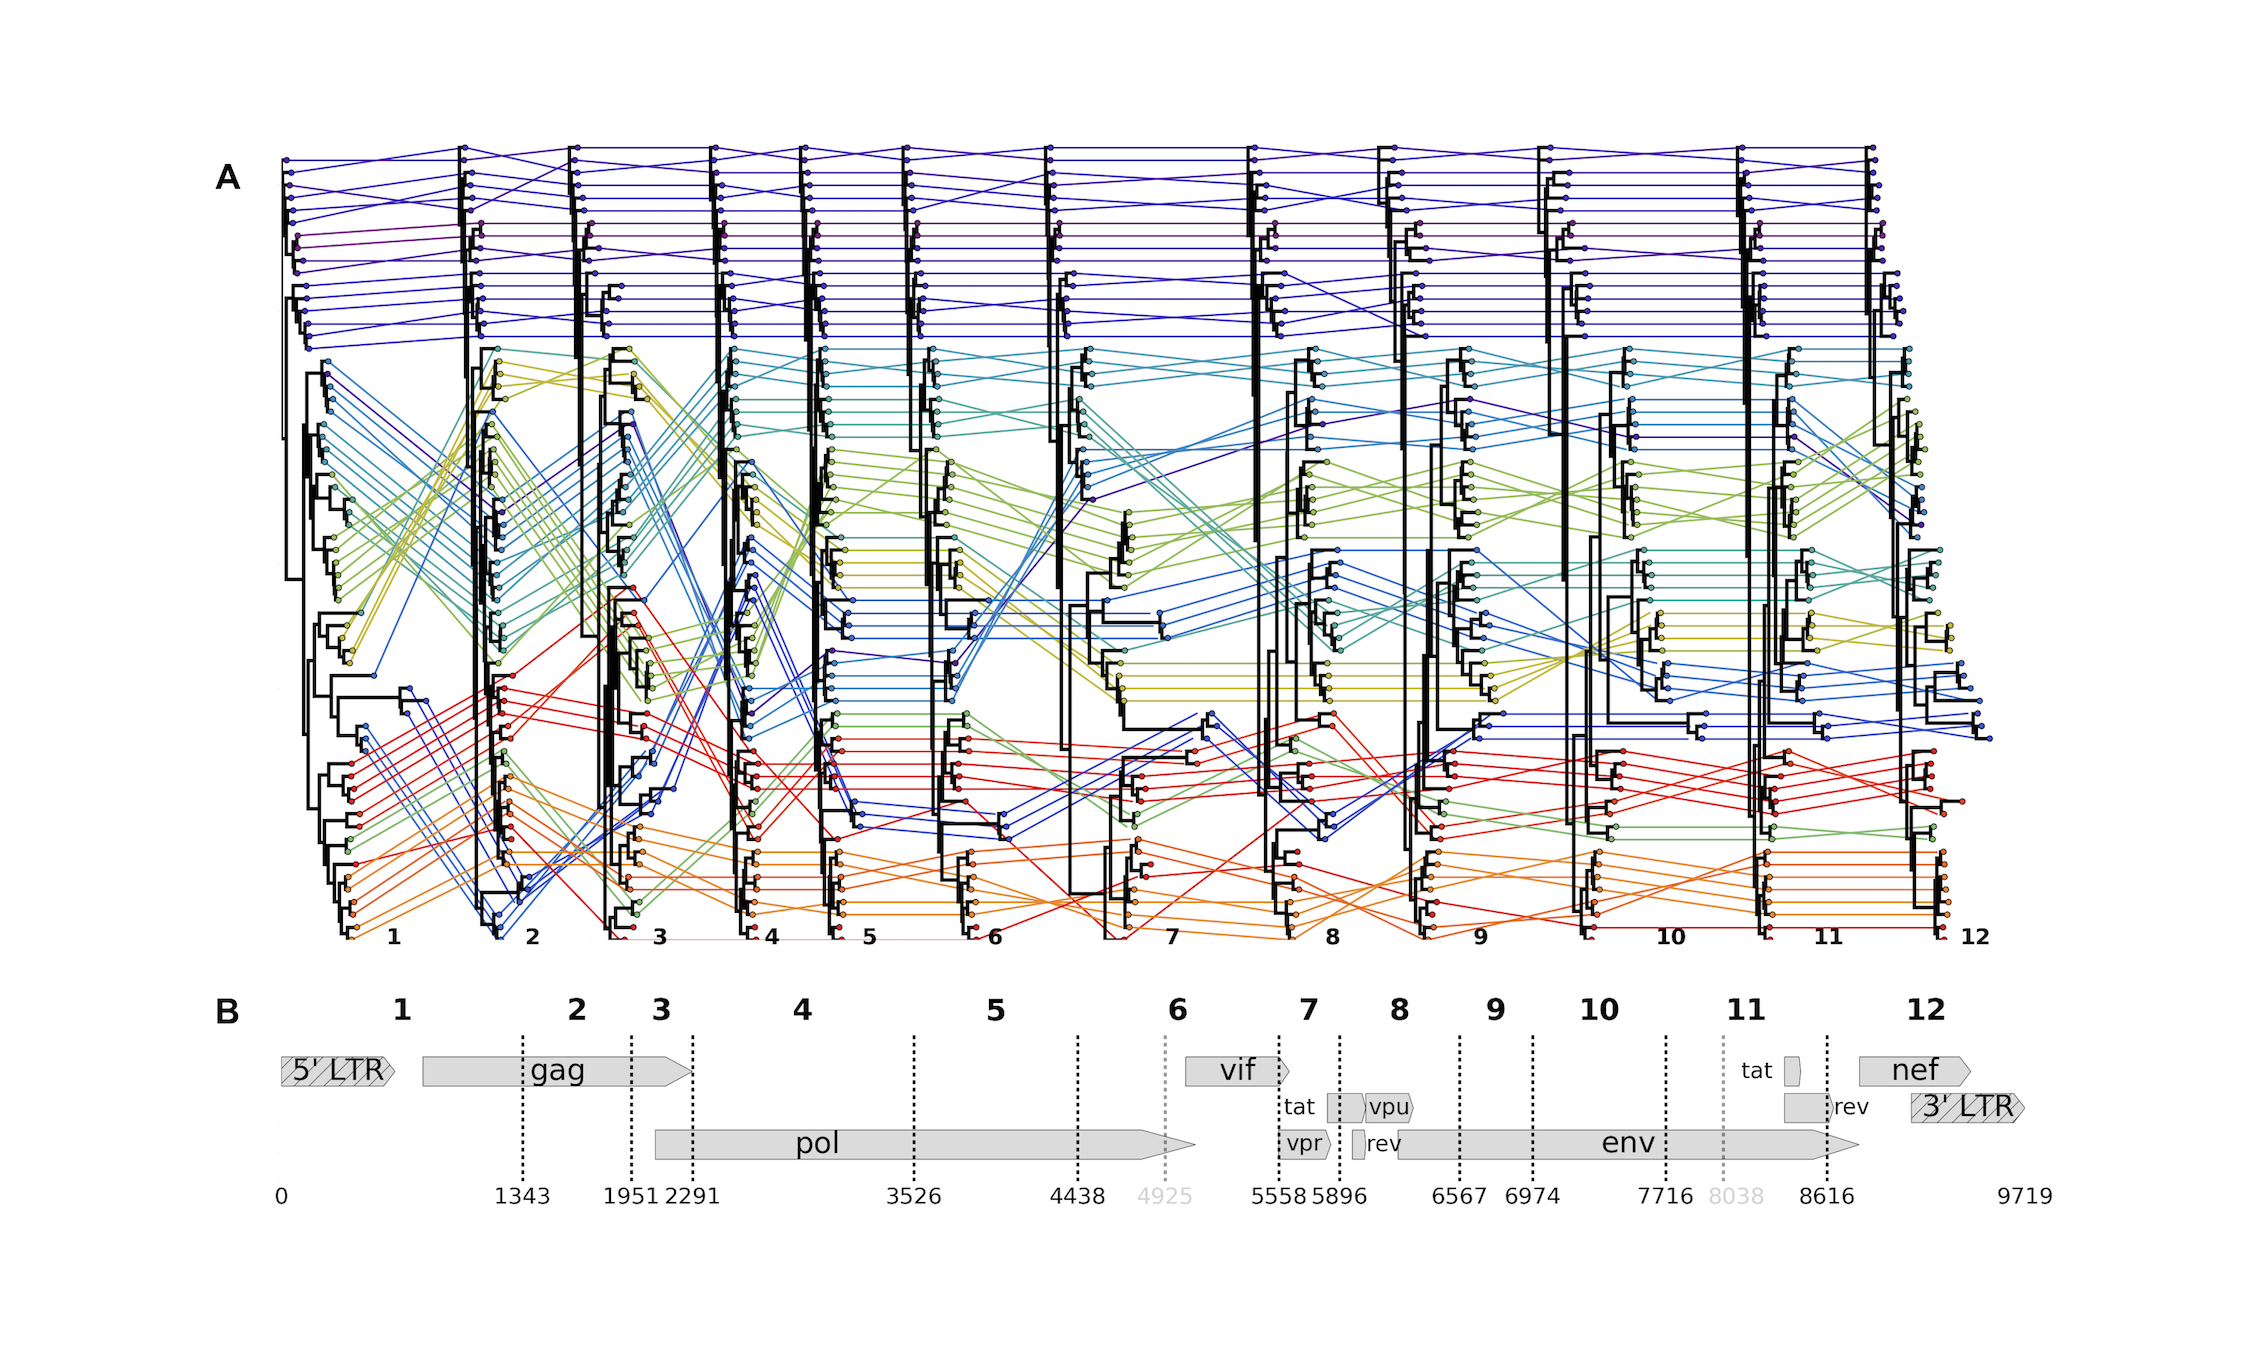
\includegraphics[width=\linewidth]{./png/siv_recombination.png}
  	\caption{\textbf{Inferred interlineage recombination breakpoints and supporting tree topologies }
The SIV LANL compendium, slightly modified to reduce overrepresentation of HIV, was analyzed with GARD to identify 13 recombination breakpoints across the genome (dashed lines in \textbf{B}; numbering according to the accepted HXB2 reference genome--accession K03455, illustrated).
Two of these breakpoints were omitted from further analyses because they created extremely short fragments (< 500 bases; gray dashes in \textbf{B}).
For each of the 11 remaining breakpoints used in further analyses, we split the compendium alignment along these breakpoints and built a maximum likelihood tree, displayed in \textbf{A}.
Each viral sequence is color-coded by host species, and its phylogenetic position is traced between trees.
Heuristically, straight, horizontal colored lines indicate congruent topological positions between trees (likely not a recombinant sequence); criss-crossing colored lines indicate incongruent topological positions between trees (likely a recombinant sequence).
    }
  	\label{siv_recombination}
  \end{centering}
\end{figure}

GARD identified 13 locations along the genome that had strong evidence of inter-lineage recombination (Figure~\ref{siv_recombination}).
Here, evidence for a particular model is assessed via Akaike Information Criterion (AIC) and differences in AIC between models indicate log probabilities, so that a delta-AIC of 10 between two models would indicate that one model is e10/2 = ~148 as likely as the other \citep{akaike1992information}.
In our case, delta-AIC values ranged from 154 to 436 for each included breakpoint, indicating that these breakpoints are strongly supported by the underlying tree likelihoods.
The 14 resulting segments ranged in length from 351 to 2316 bases; in order to build reliable phylogenies, we omitted two of the less supported breakpoints from downstream analyses, yielding 12 segments ranging in length from 606 – 2316 bases.
We found no evidence to suggest linkage between non-neighboring segments (Fig. S2).
While it has been previously appreciated that several lineages of SIV are recombinant products (e.g., \citep{bailes2003hybrid,jin1994mosaic}), the 13 breakpoints identified here provide evidence that there have been at least 13 inter-lineage recombination events during the evolution of SIVs.
Identifying these recombination breakpoints allowed us to construct a putatively valid phylogeny for each segment of the genome that shares an internally cohesive evolutionary history.

% \end{fold}

\section{Phylogenetic evidence of SIV cross-species transmission}
% \begin{fold}
We then looked for phylogenetic evidence of cross-species transmission in the tree topologies of each of the 12 genomic segments.
For this and all further analyses, we constructed a dataset from all publicly available primate lentivirus sequences, which we curated and subsampled by host and virus lineage to ensure an equitable distribution of data (see Methods).
This primary dataset consists of virus sequences from the 24 primate hosts with sufficient data available (5 – 25 sequences per viral lineage, N=423, Fig. S3).
Alignments used the fixed compendium alignment as a template (see Methods).

In phylogenetic trees of viral sequences, cross-species transmission appears as a mismatch between the host of a virus and the host of that virus’s ancestor.
To identify this pattern and estimate how frequently each pair of hosts has exchanged lentiviruses, we used the established methods for modeling evolution of discrete traits, as implemented in BEAST \citep{faria2013simultaneously,lemey2009bayesian}.
In our case, the host of each viral sample was modeled as a discrete trait.
This is analogous to treating the “host state” of each viral sample as an extra column in an alignment, and inferring the rate of transition between all pairs of host states along with inferring ancestral host states across the phylogeny.
This approach is similar to common phylogeographic approaches that model movement of viruses across discrete spatial regions \citep{volz2013viral} and has previously been applied to modeling discrete host state in the case of rabies virus \citep{faria2013simultaneously}.
Here, we took a fully Bayesian approach and sought the posterior distribution across phylogenetic trees, host transition rates and ancestral host states.
We integrate across model parameters using Markov chain Monte Carlo (MCMC).
The resulting model provides phylogenetic trees for each segment annotated with ancestral host states alongside inferred transition rates.

\begin{figure}[h]
  \begin{centering}
    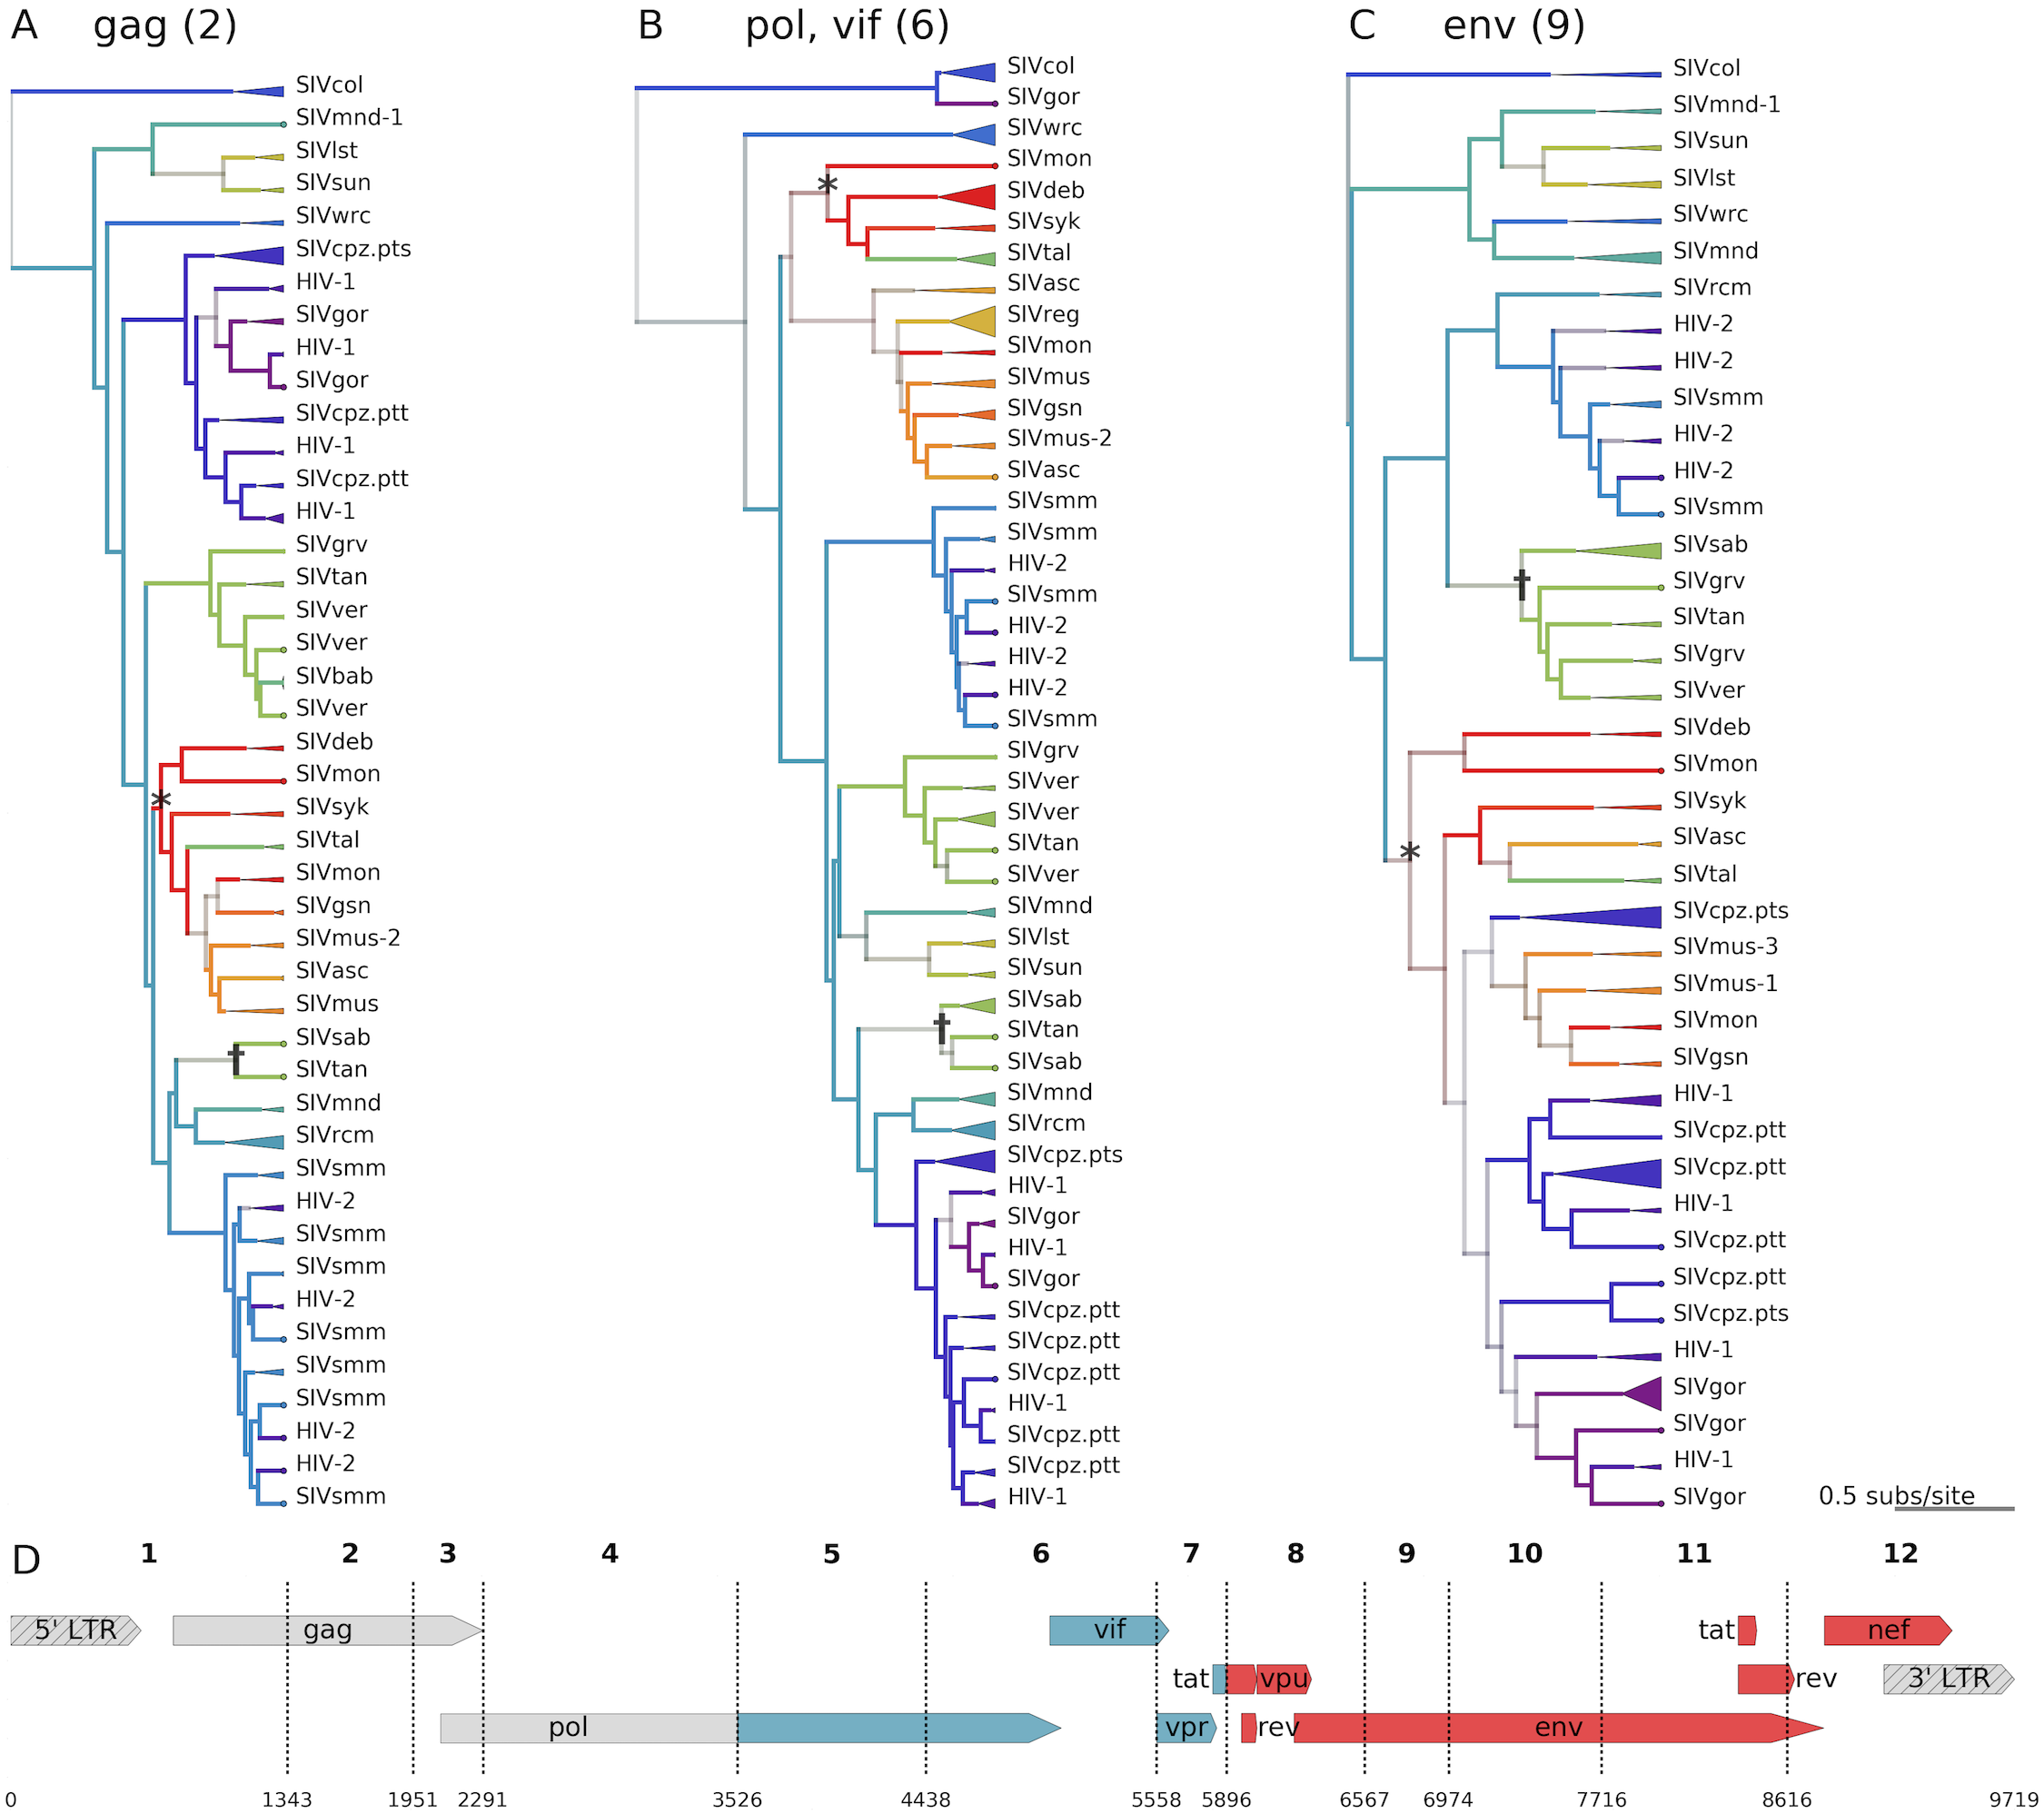
\includegraphics[width=\linewidth]{./png/siv_cpz.png}
  	\caption{\textbf{Lentiviral phylogenies highlighting the mosaic origins of SIVcpz and examples of how CST is inferred from the phylogenies }
\textbf{A,B,C} Bayesian maximum clade credibility (MCC) trees are displayed for segments 2 (gag - A), 6 (int and vif - B), and 9 (env – C) of the main dataset (N=423).
Tips are color coded by known host species; internal nodes and branches are colored by inferred host species, with saturation indicating the confidence of these assignments.
Monophyletic clades of viruses from the same lineage are collapsed, with the triangle width proportional to the number of represented sequences.
An example of likely cross-species transmission is starred in each tree, where the host state at the internal node (red / mona monkeys) is incongruent with the descendent tips' known host state (green / talapoin monkeys), providing evidence for a transmission from mona monkeys to talapoin monkeys.
Another example of cross-species transmission of a recombinant virus among African green monkeys is marked with a dagger.
\textbf{D} The genome map of SIVcpz, with breakpoints used for the discrete trait analysis, is color coded and labeled by the most likely ancestral host for each segment of the genome.
}
  	\label{siv_cpz}
  \end{centering}
\end{figure}


Figure~\ref{siv_cpz} shows reconstructed phylogenies for 3 segments along with inferred ancestral host states.
Trees are color coded by known host state at the tips, and inferred host state at internal nodes/branches; color saturation indicates the level of certainty for each ancestral host assignment.
A visual example of how the model identifies cross-species transmissions can be seen in the SIVmon/SIVtal clade, which infect mona- and talapoin monkeys, respectively (starred in Figure~\ref{siv_cpz}A-C).
Due to the phylogenetic placement of the SIVmon tips, the internal node at the base of this clade is red, indicating that the host of the ancestral virus was most likely a mona monkey.
This contrasts with the host state of the samples isolated from talapoin monkeys (tips in green).
These changes in the host state across the tree are what inform our estimates of the rate of transmission between host pairs.
In total, the support for each possible transmission is derived from both A) whether the transmission is supported across the posterior distribution of phylogenies for a particular segment, and B) whether this is true for multiple genomic segments.

Notably, the tree topologies are substantially different between segments, which emphasizes both the extent of recombination and the different evolutionary forces that have shaped the phylogenies of individual portions of the genome.
In all segments’ trees, we also see frequent changes in the host state between internal nodes (illustrated as changes in color going up the tree), suggestive of frequent ancient cross-species transmissions.
On average, primate lentiviruses switch hosts once every 6.25 substitutions per site per lineage across the SIV phylogeny.

\begin{figure}[h]
  \begin{centering}
    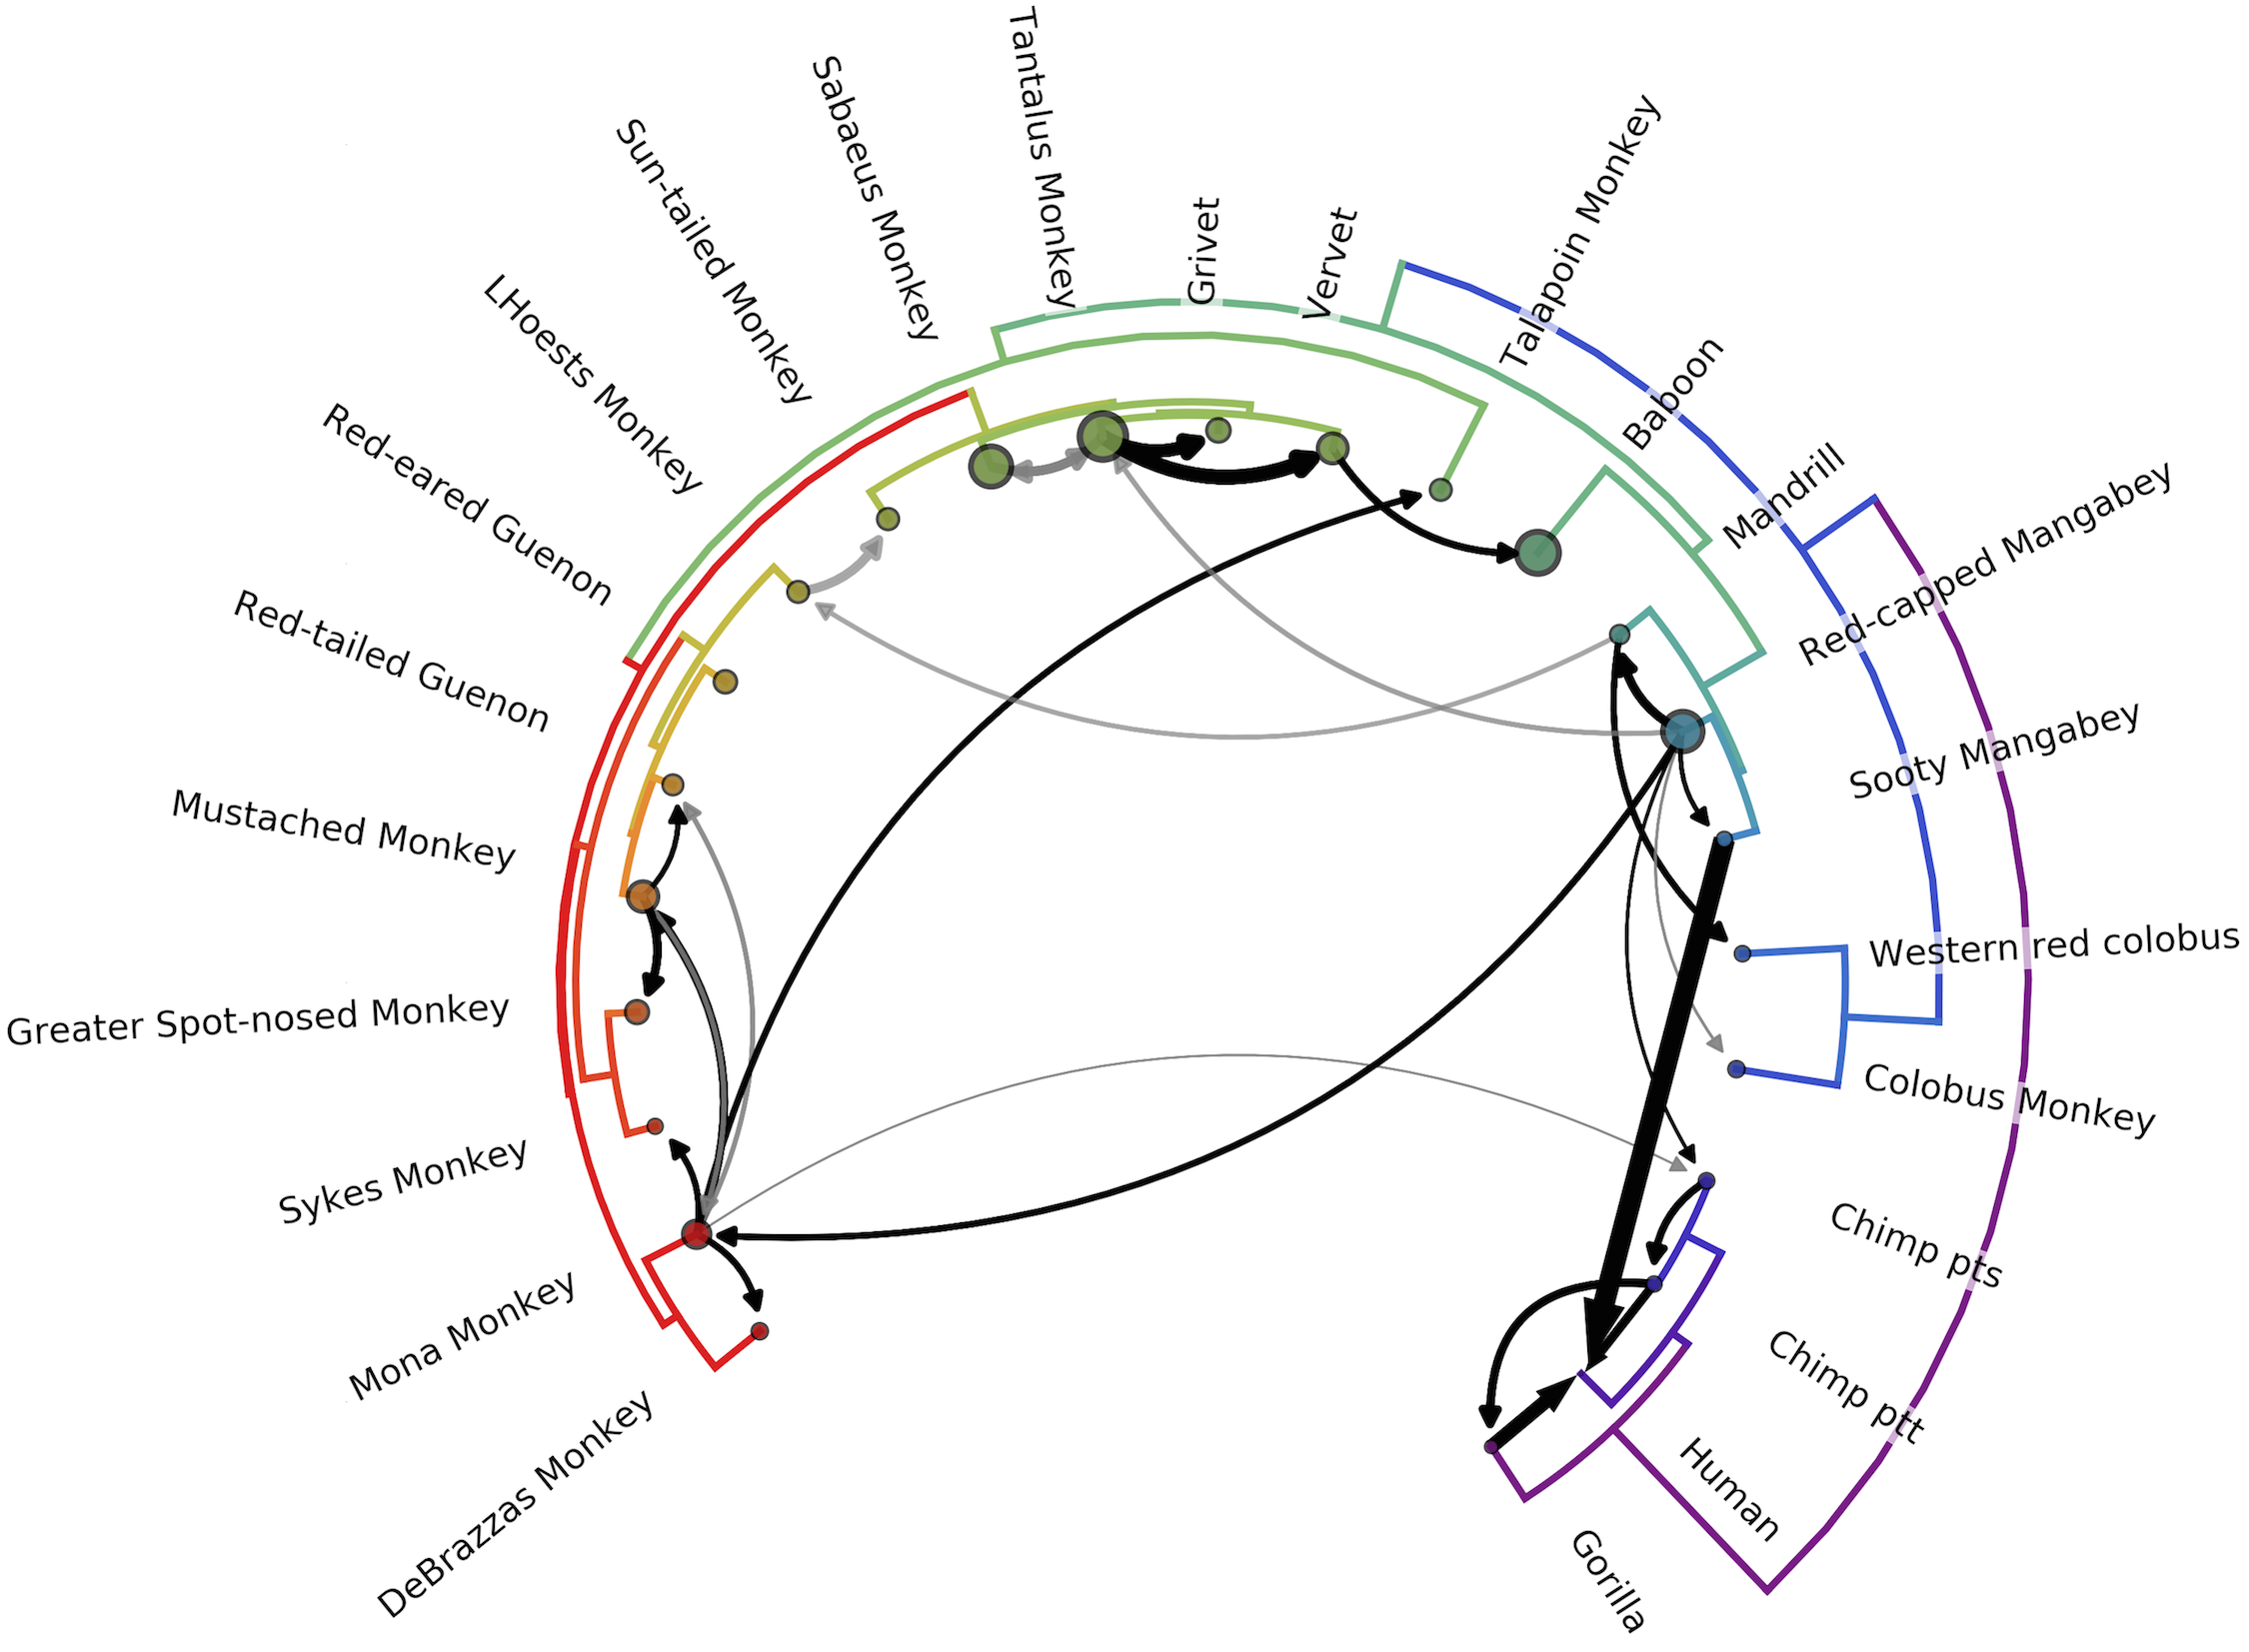
\includegraphics[width=\linewidth]{./png/siv_cst.png}
  	\caption{\textbf{Network of inferred CSTs of primate lentiviruses }
The phylogeny of the host species' mitochondrial genomes forms the outer circle.
Arrows represent transmission events inferred by the model with Bayes' factor (BF) >= 3.0; black arrows have BF >= 10, with opacity of gray arrows scaled for BF between 3.0 and 10.0.
Width of the arrow indicates the rate of transmission (actual rates = rates * indicators).
Circle sizes represent network centrality scores for each host.
Transmissions from chimps to humans; chimps to gorillas; gorillas to humans; sooty mangabeys to humans; sabaeus to tantalus; and vervets to baboons have been previously documented.
To our knowledge, all other transmissions illustrated are novel identifications.
    }
  	\label{siv_cst}
  \end{centering}
\end{figure}


The cross-species transmission events inferred by the model are illustrated in Figure~\ref{siv_cst}, with raw rates and Bayes factors (BF) in Fig. S4.
As shown, the model correctly infers nearly all pairs of hosts with previously identified (to our knowledge) CST events \citep{bailes2003hybrid,d2015origin,gao1992human,gao1999origin,jin1994infection,leitner2007sequence}, with the exception of the putative CST from sooty mangabeys to sabaeus monkeys reported by \citep{jin1994mosaic} (see discussion).
Importantly, we also identify 14 novel cross-species transmission events with strong statistical support (cutoff of BF >= 10.0).
Each of these transmissions is clearly and robustly supported by the tree topologies (all 12 trees are illustrated in %Fig. #).

To control for sampling effects, we repeated the analysis with a supplemental dataset built with fewer hosts, and more sequences per host (15 host species, subsampled to 16-40 sequences per viral lineage, N=510), and see consistent results.
As illustrated in Figs. S6-8, we find qualitatively similar results.
When directly comparing the average indicator values, host state transition rates, and BF values between analyses, the results from the main and supplemental datasets are strongly correlated, indicating robust quantitative agreement between the two analyses (Fig. S9).
We also see similar agreement between replicates when we regenerate the main dataset via independent sampling draws (see online repository).

Taken together, these results represent a far more extensive pattern of CST among primate lentiviruses than previously described \citep{apetrei2004history,sharp2011origins}; nearly every primate clade has at least one inbound, robustly supported viral transmission from another clade.
We thus conclude that the majority of lentiviruses have arisen from a process of host switching, followed by a combination of intraclade host switches and host-virus coevolution.

% \end{fold}

\section{Variable host specificity of SIVs}
% \begin{fold}
While most SIVs are the product of ancient recombination and host switching, the distribution of these host switches is not uniform; when we assess the network centrality of each virus we find a broad range (Figures~\ref{siv_cst}, S7, S11, as node size), indicating some hosts act as sources in the SIV transmission network and other hosts act as sinks.
From this, we infer that some viruses have either had greater opportunity or have a greater ability to cross the species barrier than others.

In particular, the SIVs from the four closely related species of African green monkeys (SIVsab, SIVtan, SIVver, SIVgrv; collectively, SIVagm) appear to exchange viruses with other host species frequently (Figure~\ref{siv_cst}, 12’ o-clock).
An example of SIVagm CST events can be seen in the tree topologies from gag, prot, reverse transcriptase (RT), and vif (Figures~\ref{siv_cpz} and S5, segments 2, 3, 4, 6).
Here, SIVtan isolates reported by Ayouba et al. \citep{ayouba2015molecular} (denoted with ✝ in Figure~\ref{siv_cpz}) clearly cluster with SIVsab, in a distant part of the phylogeny from the rest of the SIVagm viruses (including the majority of SIVtan isolates).
For all other segments, however, the SIVagms cluster together.
We thus concur with the conclusion of Ayouba et al. that these samples represent a recent spillover of SIVsab from sabaeus monkeys to tantalus monkeys, and the model appropriately identifies this transmission.

Contrastingly, previous studies of the lentiviral phylogeny have noted that SIVcol is typically the outgroup to other viral lineages, and have hypothesized that this may implicate SIVcol as the “original” primate lentivirus \citep{compton2013convergence}.
We find this hypothesis plausible, but the evidence remains inconclusive.
For the majority of genomic segments, we also observe SIVcol as the clear outgroup (Figures~\ref{siv_cpz} and S5).
In contrast, for portions of gag/pol (segments 3 and 4) and some of the accessory genes (segment 7), we find that there is not a clear outgroup.
For these segments, many other lineages of SIV are just as closely related to SIVcol as they are to each other.
However, with the occasional exception of single heterologous taxa with poorly supported placement, SIVcol remains a monophyletic clade (N=16), and does not intercalate within the genetic diversity of any other lineage in our dataset.
Based on these collective tree topologies, our model does not identify strong evidence for any specific transmissions out of colobus monkeys, and identifies only a single, weakly supported inbound transmission (likely noise in the model caused by the fact that red-capped mangabeys are the marginally supported root host state; see below).
This is consistent with previous findings that the colobinae—in a different genus than most of the Cercopithecus primates in our dataset—have a unique variant of the APOBEC3G gene, which is known to restrict lentiviral infection and speculated to be a barrier to cross-species transmission \citep{compton2013convergence}.
These observations generally support the idea of SIVcol as having maintained a specific relationship with its host over evolutionary time.

Additionally, while most host species carry only one lineage of SIV, mandrils and mustached monkeys carry 2 and 3 lineages of SIV, respectively \citep{aghokeng2007full,courgnaud2003identification,liegeois2012new,souquiere2001wild}.
In agreement with these previous studies, SIVmnd-1 and SIVmnd-2 do not always cluster together in the phylogeny; the same is true for SIVmus-1, SIVmus-2, and SIVmus-3, indicating that each of these viral lineages likely has a unique origin.
This stands in stark contrast to baboons, which have only been infected by an SIV via a single documented spillover event \citep{jin1994infection}.

Collectively, these examples demonstrate that the nature of the host-virus relationship is highly variable for primate lentiviruses, with some viruses switching hosts often while others putatively maintain strict host specificity.
Likewise, while some hosts have acquired multiple SIV lineages, most are infected by only one SIV, or do not have an endemic SIV.

% \end{fold}

\section{The evolutionary history of SIVcpz, the precursor to HIV-1}
% \begin{fold}
Unlike SIVcol, SIVcpz appears to be the product of multiple CSTs and recombination events.
SIVcpz actually encompasses two viral lineages: SIVcpzPtt infects chimpanzees of the subspecies Pan troglodytes troglodytes, and SIVcpzPts infects chimpanzees of the subspecies Pan troglodytes schweinfurthii \citep{santiago2002sivcpz}.
There are two additional subspecies of chimpanzees that have not been found harbor an SIV despite extensive surveys, suggesting that SIVcpzPtt was acquired after chimpanzee sub-speciation \citep{leitner2007sequence}.
Both this previous work and our own results support the hypothesis that SIVcpz was later transmitted from one chimpanzee subspecies to the other, and SIVcpzPtt is the only SIVcpz lineage that has crossed into humans.
Given the shared ancestry of the two lineages of SIVcpz, we use “SIVcpz” to refer specifically to SIVcpzPtt.

Based on the lentiviral sequences available in 2003, Bailes et al \citep{bailes2003hybrid} suggested that the SIVcpz genome is a recombinant of just two parental lineages.
SIVrcm (which infects red-capped mangabeys) was identified as the 5’ donor, and an SIV from the SIVmon/-mus/-gsn clade (which infect primates in the Cercopithecus genus) was identified as the 3’ donor.
Since the time of this previous investigation many new lentiviruses have been discovered and sequenced.
In incorporating these new data, we find clear evidence that the previous two-donor hypothesis may be incomplete.

The tree topologies from env in the 3’ end of the genome (segments 8-11) support the previous hypothesis \citep{bailes2003hybrid} that this region came from a virus in the SIVmon/-mus/-gsn clade.
These viruses form a clear sister clade to SIVcpz with high posterior support (Figure~\ref{siv_cpz}C,D).
We find strong evidence for transmissions from mona monkeys (SIVmon) to mustached monkeys (SIVmus), and from mustached monkeys to greater spot-nosed monkeys (SIVgsn) (see discussion of potential coevolution below).
We also find more evidence in support of a transmission from mona monkeys to chimpanzees than from the other two potential donors, but more sampling is required to firmly resolve which of these viruses was the original donor of the 3’ end of SIVcpz.

We find phylogenetic evidence to support the previous hypothesis \citep{bailes2003hybrid,etienne2013gene} that the integrase and vif genes of SIVcpz (segments 4-6) originated from SIVrcm; however, we find equally strong evidence to support the competing hypothesis that pol came from SIVmnd-2, which infects mandrils (Figure~\ref{siv_cpz}B,D).
In these portions of the genome, SIVmnd-2 and SIVrcm together form a clear sister clade to SIVcpz.
The vpr gene, in segment 7, is also closely related to both SIVrcm and SIVmnd-2, but this sister clade also contains SIVsmm from sooty mangabeys.
Notably, we infer a transmission from red-capped mangabeys to mandrils, but we cannot determine whether this portion of the SIVcpz genome was acquired directly from SIVrcm or from SIVmnd-2.

Interestingly, we do not find evidence to support either SIVrcm/mnd-2 or SIVmon/mus/gsn as the donor for the 5’ most end of the genome (segments 1-5), including the 5’ LTR, gag, and RT genes.
This is also true for the 3’ LTR (segment 12).
SIVcpz lacks a clear sister clade or ancestor in this region, and SIVrcm groups in a distant clade; we therefore find no evidence to suggest that an ancestor of an extant SIVrcm was the parental lineage of SIVcpz in the 5’ most end of the viral genome as previously believed (Figure~\ref{siv_cpz}A,D).
This may support the possibility of a third parental lineage, or a number of other plausible scenarios (discussed below).

% \end{fold}

\section{Discussion}
% \begin{fold}

\subsection*{Limitations and strengths of the model}
\textbf{Additional sampling is required to fully resolve the history of CST among lentiviruses}\\
In addition to the 14 strongly supported novel transmissions (BF >= 10) described above, we also find substantial evidence for an additional 8 possible novel transitions, but with lower support (BF >= 3) (Figures~\ref{siv_cst}3, S4).
These transmissions are more difficult to assess, because many of them are inferred on the basis of just a few “outlier” tips of the tree that group apart from the majority of viral samples from the same lineage.
In each case, the tips’ phylogenetic position is strongly supported, and the primary literature associated with the collection of each of these “outlier” samples clearly specifies the host metadata.
However, due to the limited number of lentiviral sequences available for some hosts, we are unable to control for sampling effects for some of these lower-certainty transmissions.
We report them here because it is unclear whether these outliers are the result of unidentified separate endemic lineages, one-time spillovers from other hosts, or species misidentification during sample collection.
It is also important to note that while some of these less-supported transmissions are potentially sampling artifacts, many of them may be real, and may be less supported simply because they lack the requisite available data for some genome segments.

Ultimately, far more extensive sampling—specifically, obtaining more full-length sequences from undersampled lineages—of primate lentiviruses is required in order to resolve these instances.
We included only sequences at least 500 bases long; each taxon may contribute more informative sites to some segments than to others.
When splitting the master alignment along breakpoints, we removed from each segment any taxon that had no informative bases.
However, for each segment, there were between 0 and 13 (mean: 3.6) taxa that had some informative sites, but were very short (<100 informative sites).
Statistically, these short taxa contribute little information, and are placed in the topology for each segment with high uncertainty.
This phylogenetic uncertainty is then propagated forward to the discrete traits model, meaning that these short taxa should not statistically influence our results in any meaningful way.
Notably, though, their removal does result in extensive technical challenges (this “pruned” dataset results in poor mixing and rather divergent results, seen in Figs. S10-12).
Given the high congruence between results from independent sampling replicates of the main dataset and from an alternative sampling scheme, we believe this to be a technical issue, rather than reflecting true differences.
However, this issue does further emphasize the importance of additional sampling in fully resolving the natural history of SIVs.

\textbf{Most lentiviruses were originally acquired by CST and have since coevolved with their hosts}\\
Some of these “noisier” transmission inferences, particularly within the same primate clade, may be the result of coevolution, i.e. lineage tracking of viral lineages alongside host speciation.
Within the model, viral jumps into the common ancestor of two extant primate species appear as a jump into one of the extant species, with a secondary jump between the two descendants.
For example, the model infers a jump from mona monkeys into mustached monkeys, with a secondary jump from mustached monkeys into their sister species, red-tailed guenons (Figure~\ref{siv_cst}).
Comparing the virus and host phylogenies, we observe that this host tree bifurcation between mustached monkeys and red-tailed guenons is mirrored in the virus tree bifurcation between SIVmus and SIVasc for most segments of the viral genome (Figures~\ref{siv_cpz}, \ref{siv_cst}).
This heuristically suggests that the true natural history may be an ancient viral transmission from mona monkeys into the common ancestor of mustached monkeys and red-tailed guenons, followed by host/virus coevolution during primate speciation to yield SIVmus and SIVasc.
The possibility of virus/host coevolution means that while we also observe extensive host switching between primate clades, many of the observed jumps within a primate clade may be the result of host-virus coevolution.
However, we also note that the species barrier is likely lower between closely related primates, making it challenging to rigorously disentangle coevolution vs. true host switches within a primate clade \citep{charleston2002preferential}.

\textbf{The model propagates and accounts for residual uncertainty from the recombination analyses}\\
The deep phylogenies and extensive sequence divergence between SIV lineages makes any assessment of recombination imperfect.
Our analysis aims to 1) place a lower bound on the number of interlineage recombination events that must have occurred to explain the observed extant viruses, and 2) use this understanding to construct a model of CST among these viruses.
As the most well developed package currently available for topology-based recombination analysis, GARD was an appropriate choice to identify in broad strokes the extent and nature of recombination among SIVs.
Some (though not all) of the remaining uncertainty as to the exact location of breakpoints is represented within the posterior distribution of trees for each segment, and is thus propagated and accounted for in the discrete traits model (inferences of CST).
Most other studies of SIV evolutionary history simply split the phylogeny along gene boundaries or ignore recombination (e.g., \citep{bailes2003hybrid,charleston2002preferential,sharp2011origins}).
Thus, while there is still some remaining uncertainty in our recombination analyses, these results still represent a major step forward in attempting to systematically assess recombination among all extant SIV lineages and to incorporate it into the phylogenetic reconstruction.

\subsection*{Cross-species transmission is driven by exposure and constrained by host genetic distance}
Paleovirology, biogeography, and statistical models of lentiviral evolution estimate that primate lentiviruses share a common ancestor approximately 5-10 million years ago \citep{aiewsakun2016time,compton2013convergence,mccarthy2015evolutionary,worobey2010island}.
This, along with the putative viral coevolution during primate speciation, suggests that many of these transmissions were ancient, and have been acted on by selection for millions of years.
Thus, given that the observed transmissions almost exclusively represent evolutionarily successful host switches, it is remarkable that lentiviruses have been able to repeatedly adapt to so many new host species.
In the context of this vast evolutionary timescale, however, we conclude that while lentiviruses have a far more extensive history of host switching than previously understood, these events remain relatively rare overall.
As noted above, our results illustrate that some SIVs cross the species barrier more readily than others, and some primate host species become infected with new viral lineages more commonly than others.
This is likely governed by both ecological and biological factors.
Ecologically, frequency and form of exposure are likely key determinants of transmission \citep{locatelli2012cross}, but these relationships can be difficult to describe statistically.

\begin{figure}[h]
  \begin{centering}
    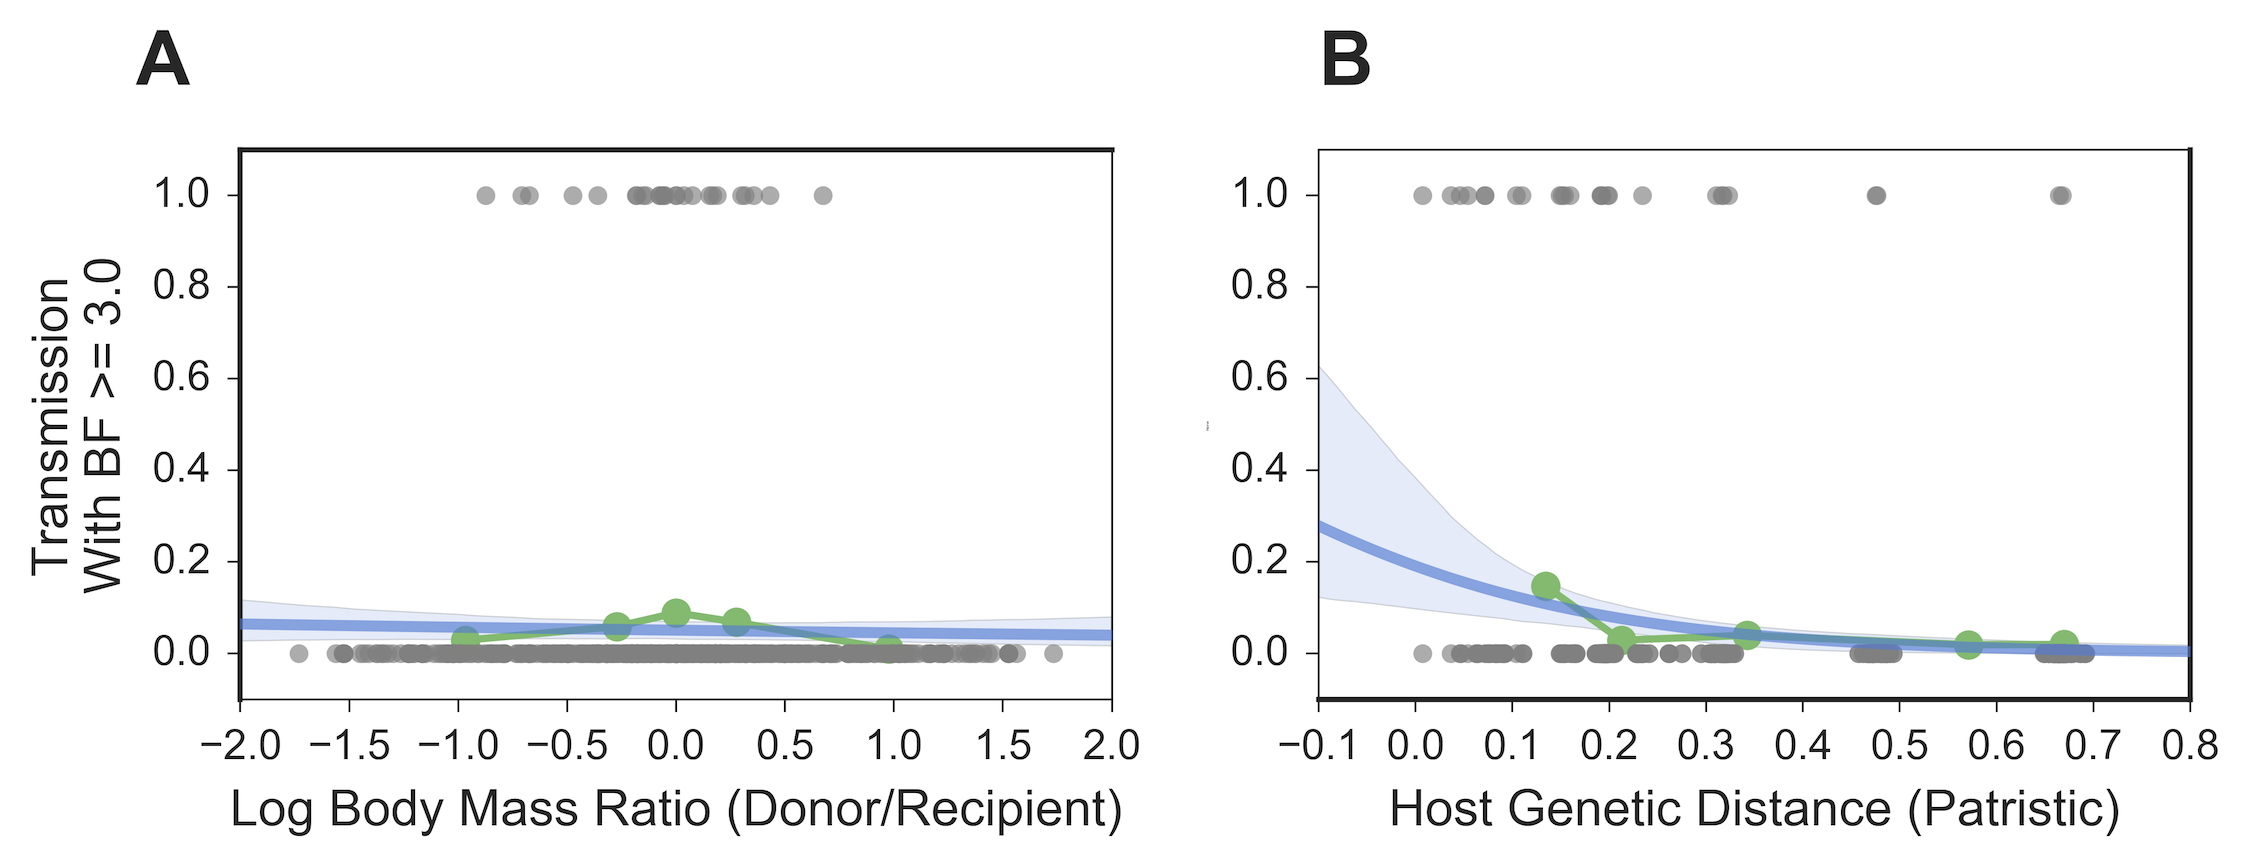
\includegraphics[width=\linewidth]{./png/siv_predict.png}
  	\caption{\textbf{Logistic regressions of body mass ratios (a proxy for predation) and host genetic distance on the probability of CST }
For each pair of host species, we \textbf{(A)} calculated the log ratio of their average body masses and \textbf{(B)} found the patristic genetic distance between them (from a maximum-likelihood tree of mtDNA).
To investigate the association of these predictors with cross-species transmission, we treated transmis-sion as a binary variable: 0 if the Bayes factor for the transmission (as inferred by the discrete traits model) was < 3.0, and 1 for a Bayes factor >= 3.0.
Each plot shows raw predictor data in gray; the quintiles of the predictor data in green; and the logistic regression and 95% CI in blue.
    }
  	\label{siv_predict}
  \end{centering}
\end{figure}

For example, many primates are chronically exposed to many exogenous lentiviruses through predation \citep{aghokeng2010extensive,goodall1986chimpanzees,sharp2011origins}.
Using log body mass ratios \citep{iucn2008international} as a proxy for predation, we do not see a statistically significant association between body mass ratio and non-zero transmission rate (Figure~\ref{siv_predict}A, blue; p=0.678, coef. 95\% CI (-0.311, 0.202)).
We believe the lack of signal is likely due to the imperfect proxy, although it is also possible that predator-prey relationships do not strongly structure the CST network.
It is also likely that geographic overlap and habitat similarity are ecological determinants of SIV CST, but modern primate habitats are likely very different since the time that these transmissions actually occurred.

Biologically, increasing host genetic distance has a clear negative association with the probability of cross-species transmission (Figure~\ref{siv_predict}B, blue, p<0.001, coef. 95\% CI [-7.633, -2.213]).
Importantly, as already discussed, the strength of this association may be inflated by instances of lineage tracking (virus/host cospeciation).
However, it is well established that increasing host genetic distance is associated with a higher species barrier \citep{charleston2002preferential}.
As previously documented in the literature we expect this is due to several factors, such as the divergence of host restriction factor genes, which are key components of the innate immune system (reviewed in \citep{harris2012restriction}) and differences in host cell receptor phenotypes (e.g., \citep{chen1998natural,pandrea2007paucity,riddick2010novel}).
Functional assays of these host phenotypes against panels of SIVs, while outside the scope of this study, will be important for further identifying the molecular bases of the species barriers that have led to the transmission patterns identified here.

\subsection*{Origins of HIV-1 and HIV-2}
\textbf{Epidemiological factors were key to the early spread of HIV}\\
Understanding the underlying dynamics of lentiviral CST provides important ecological context to the transmissions that generated the HIV pandemic.
As discussed above, our results support a view of lentiviral cross-species transmission as a rare event.
Notably, only two lentiviruses have crossed the high species barrier from Old World monkeys into hominids: SIVsmm and the recombinant SIVcpz.
Both HIV-1 and HIV-2 have arisen in human populations in the last century \citep{faria2014early,sharp2011origins}.
While it is possible that this has occurred by chance, even without increased primate exposure or other risk factors, we nevertheless find it striking that humans would acquire two exogenous viruses within such a short evolutionary timespan.
Examining this phenomenon more closely, the history of HIV-2 is enlightening.
HIV-2 has been acquired through at least 8 independent spillover events from sooty mangabeys \citep{sharp2011origins}.
Notably, 6 of these transmissions have resulted in only a single observed infection (spillovers) \citep{chen1996genetic,chen1997human,gao1992human}; only 2 of these events have established sustained transmission chains and successfully switched hosts to become endemic human pathogens \citep{damond2001quantification,ishikawa2001genetic,pieniazek1999predominance}.
This pattern, as well as serology-based reports of other limited spillovers of SIVs into humans \citep{kalish2005central,souquiere2001wild}, suggest that there have been many isolated introductions of lentiviruses into humans over the past 200,000 years.
However, these other viral exposures did not result in new endemic human pathogens either because of species-specific immune barriers, non-conducive epidemiological conditions, or a combination thereof.
The rapid and repeated emergence of HIV-1 and HIV-2 is on a timescale more congruent with changes in epidemiological conditions than mammalian evolution, perhaps emphasizing the importance of the concurrent changes in human population structure and urbanization in facilitating the early spread of the epidemic \citep{faria2014early}.
Significantly, though, this also highlights the importance of careful public health surveillance and interventions to prevent future epidemics of zoonotic viruses.

\textbf{The exact origins of SIVcpz may not be identifiable}\\
The ancestry of SIVcpz appears to be tripartite: the unknown ancestry of the 5’ end; the putatively SIVrcm or SIVmnd-2 derived int and vif genes; and the putatively SIVgsn/mon/mus derived 3’ end of the genome.
For any of these three portions of the genome, there are multiple evolutionary histories supported by available sequence data.
However, it is possible that further sampling of lentivirus lineages (both known and currently undiscovered) will be able to definitively resolve the ancestry of SIVcpz.
Alternatively, it may be that the ancestral virus(es) that gave rise to any of these three portions is extinct \citep{apetrei2010pattern}.
In the case of the last two portions of the SIVcpz genome, it may be that the common ancestor of these putative genetic donors (SIVrcm/mnd-2 and SIVmon/mus/gsn, respectively) was the true source.
However, it is also a distinct possibility that SIVcpz has sufficiently diverged since its acquisition by chimpanzees such that its history is obscured.

\textbf{Evolutionary time obscures the identity of the “original” primate lentivirus}\\
Among primates, our results clearly illustrate that the vast majority of lentiviral lineages were originally acquired by cross-species transmission.
It is intriguing to speculate as to which virus was the “original” source of all of these lineages.
Because of its consistent position as the outgroup of primate lentiviral trees, it has been hypothesized \citep{compton2013convergence} that SIVcol was this original lentivirus among primates.
While SIVcol is certainly the most evolutionary isolated extant lentivirus that has been sampled to date, this does not definitively place it as the ancestral lentivirus.
Alternative scenarios (also noted by \citep{apetrei2010pattern,compton2013convergence}) include an extinct original lentiviral lineage (and/or primate host species) or an unsampled ancestral lentivirus.
It is also plausible that another known extant lentivirus was the “original” lineage, but has diverged and/or recombined to such an extant that its origins are obscured.

\subsection*{Conclusions}
Here, we have shown that lentiviruses have a far more extensive history of host switching than previously described.
Our findings also demonstrate that the propensity of each lentiviral lineage to switch between distant hosts, or to spillover among related hosts, is highly variable.
In examining specific lineages, our findings are consistent with the prevalent hypothesis that SIVcol has evolved in isolation from other SIVs.
Contrastingly, we have also demonstrated that the mosaic origins of SIVcpz are far more complex than previously recognized; the currently available sequence data is unable to resolve the ancestry of nearly half of the SIVcpz genome.
Together, our analyses move closer to a full understanding of the pattern of cross-species transmission among primate lentiviruses, but additional efforts to obtain high quality viral genome sequences from under sampled lineages will be necessary to fully resolve the natural history of these viruses.
% \end{fold}


\section{Methods}
% \begin{fold}
\subsection*{Datasets \& alignments}
Lentiviral genomes are translated in multiple reading frames; we therefore utilized nucleotide sequence data for all analyses.

\textbf{Recombination analysis dataset}\\
For all recombination analyses (GARD, R2, rSPR), we used the 2015 Los Alamos National Lab (LANL) HIV/SIV Compendium \citep{los2012hiv}.
The compendium is a carefully curated alignment of high-quality, representative sequences from each known SIV lineage and each group of HIV-1 and HIV-2.
We reduced the overrepresentation of HIV in this dataset, but maintained at least one high quality sample from each group of HIV.
In total, this dataset contains 64 sequences from 24 hosts (1-10 sequences per host).
Maximum likelihood trees for each segment—used for the rSPR analysis and displayed in Figure~\ref{siv_recombination}—were built with RAxML v.8.2.9 \citep{stamatakis2014raxml} with the rapid bootstrapping algorithm under a GTR model with 25 discrete bins of site to site rate variation and were rooted to SIVcol for display.

\textbf{Main \& supplemental datasets}\\
Primate lentiviral sequences were downloaded from the comprehensive LANL HIV sequence database \citep{los2012hiv}.
Sequences from lineages known to be the result of artificial cross-species transmissions (SIVmac, -stm, -mne, and –wcm) were excluded.
We also excluded any sequences shorter than 500 bases or that were flagged as problematic by standard LANL criteria.
We grouped host subspecies together except for cases where there is a known specific relationship between host subspecies and virus lineage (chimpanzees and African green monkeys).
To construct datasets with a more equitable distribution of sequences per host, we preferentially subsampled sequences from the LANL Compendium, followed by samples isolated from Africa (more likely to be primary sequences), and finally supplementing with samples isolated elsewhere (excluding experimentally generated sequences).
For humans, mandrils and mustached monkeys, which are host to 2, 2 and 3 distinct viral lineages, respectively, we allowed a few additional sequences (if available) to represent the full breadth of documented lentiviral diversity.
The “main” dataset consists of 24 host species, with 5-31 sequences per host (total N=422).
As an alternative dataset to control for sampling bias and data availability, we also constructed a “supplemental” dataset with just 15 hosts but with more viral sequences per host (16 – 40 sequences per lineage, N=510).

\textbf{Alignments}\\
Alignments were done with the L-INSI algorithm implemented in mafft v7.294b \citep{katoh2013mafft}; the Compendium alignment was held fixed, with other sequences aligned to this template.
Insertions relative to the fixed compendium were discarded.
This alignment was then split along the breakpoints identified by GARD to yield the segment-specific alignments.
Sequences that contained no bases for a given seg-ment were removed; the “pruned” dataset is identical to the “main” dataset, but here we also removed sequences with fewer than 100 ungapped bases for a given segment.

\subsection*{Recombination analyses}
\textbf{Topology-based analysis}\\
Each portion of the genome was analyzed with the Genetic Algorithm for Recombination Detection (GARD), implemented in HyPhy v.2.2.0 \citep{kosakovsky2006gard}, with a nucleotide model selected by HyPhy’s Nu-cModelCompare package (\#012234) and general discrete distribution (3 bins) of site variation.
Computational intensity was eased by analyzing the recombination dataset in 3kb long portions, with 1kb overlaps on either end (e.g., bases 1:3000, 2000:5000, 4000:7000, etc.).
To control for sites’ proximity to the ends of the genomic portion being analyzed, this was repeated with the windows offset (e.g., bases 1:2500, 1500:4500, 3500:6500, etc.).
In total, this resulted in every site of the alignment being analyzed at least two-fold, with at least one of these replicates providing 500-1500 bases of genomic context on either side (other than at the very ends of the total alignment).
Disagreement between window-offset replicates for a given breakpoint were minimal and almost always agreed within a few bases, with two exceptions: offset replicates for the breakpoint between segments 7 and 8 disagreed by 529 bases, and offset replicates for the breakpoint between 8 and 9 disagreed by 263 bases.
In these instances, we used the average site placement.

\textbf{Sitewise linkage analysis}\\
Biallelic sites were identified across the genome (ignoring gap characters and polymorphisms present at <5\%).
These biallelic sites were compared pairwise to generate an observed and expected distribution of haplotypes (combinations of alleles between the two sites), and assessed with the statistic $R^2=\frac{\chi^2}{d*n}$, where $\chi^2$ is chi-square, d is the degrees of freedom, and N is the number of haplotypes for this pair of sites \citep{hill1968linkage}.
This statistic follows the canonical interpretation of $R^2$, i.e., if the allele at site 1 is known, how well does it predict the allele at site 2 (0 indicating no linkage between sites, and 1 indicating perfect linkage).

\textbf{Segment linkage analysis}\\
Segment linkage was assessed by comparing the similarity of tree topologies between segments.
This was done with the pairwise method in the Rooted Subtree-Prune-and-Regraft (rSPR) package \citep{whidden2017ricci}, which measures the number of steps required to transform one topology into another.
Segment pairs with similar topologies have lower scores than segments with less similar topologies.

\subsection*{Phylogenies \& discrete trait analysis}
\textbf{Empirical tree distributions}\\
For each segment alignment, a posterior distribution of trees was generated with BEAST v. 1.8.2 under a general time reversible substitution model with gamma distributed rate variation and a strict molecular clock \citep{drummond2012bayesian}.
We used a Yule birth-death speciation model tree prior \citep{gernhard2008using}; all other priors were defaults.
Trees were estimated using a Markov chain Monte Carlo (MCMC), and convergence was determined by visually inspecting the trace in Tracer v. 1.6.0 \citep{rambaut2014tracer}.
MCMC chain parameters and ESS values were as follows.

“Main” dataset: 25 million steps, sampled every 15,000 states, 10\% burnin removed. Posterior distribu-tion of ~1600 trees per segment. All but two effective sample size (ESS) values (segment 2: AG substi-tution rate [ESS=164] and frequencies 4 [ESS=189]) were well over 200. \\
“Pruned” dataset: 65 million steps, sampled every 15,000 states, 10\% burnin removed. Posterior distribution of ~3900 trees per segment. \\
“Resampled” dataset: 65 million steps, sampled every 15,000 states, 10\% burnin removed. Posterior distribution of ~3900 trees per segment. All ESS values except for the AG substitution rate in segment 2 (ESS=190) were well above 200.

\textbf{Discrete trait analysis}\\
These tree distributions were used to estimate the transmission network.
As in Faria et al. \citep{faria2013simultaneously}, we model hosts as states of a discrete trait, and model cross-species transmission as a stochastic diffusion process among n host states.
We use a non-reversible state transition matrix with n × (n–1) indi-vidual transition parameters \citep{edwards2011ancient}.
We also utilize standard methodology in using a Bayesian stochastic search variable selection process to encourage a sparse network, implemented as in \citep{lemey2009bayesian}.
An exponential distribution with mean=1.0 was used as a prior on each of the pairwise rate parameters (552 in total for the main and pruned datasets with 24 hosts; 210 parameters in total for the supplemental dataset with 15 hosts).
The prior placed on the sum of the binary indicator variables corresponding to each pairwise rate parameter (i.e., the number of transitions that are non-zero) was an exponential distribution with mean=20-23.
Convergence was again assessed by visually inspecting the log files in Tracer.

MCMC chain parameters and ESS values were as follows.
“Main” dataset: 25 million steps, sampled every 5,000 states, 5 million states discarded as burnin.\\
“Pruned” dataset: decreased phylogenetic noise in the empirical tree distributions for this dataset led to narrow tree distributions and poor mixing (but clear convergence).
We thus ran 40 parallel chains of 25-35 million steps each, sampled every 20,000 states (trees sampled every 50,000 states).
We discarded 10 million steps of each chain as burnin and concatenated the remaining states. \\
“Resampled” dataset: 45 million steps, sampled every 5,000 steps, 20 million steps discarded as burnin. \\
For the main and supplemental datasets, more than 97\% of the rate, indicator, and actualRate (step-wise rate*indicator values) parameters, and all other parameters, had an ESS well over 200 (most > 1000).
The pruned dataset had a posterior ESS of 677, but the component tree likelihood ESS values ranged from 57 – 287; 91\% of the rate, indicator, and actualRate parameters had an average ESS value > 200.
Statistical support for each transmission is summarized as a Bayes factor (BF), calculated by comparing the posterior and prior odds that a given rate is non-zero (i.e., that there has been any transmission between a given pair of hosts) \citep{lemey2009bayesian}.
The ancestral tree likelihoods of each of the 12 tree distributions contribute equally to the inference of a shared transmission rate matrix.
However, not every lineage has recombined along every breakpoint, which means that the tree likelihoods from each segment are not fully statistically independent.
Thus, we report conservative estimates of BF by dividing all BF values by 12.

% \end{fold}

% \end{fold}

% ========== Dengue Titer Model Chapter
\chapter{Dengue virus antigenic evolution}
% \begin{fold}

\section{Introduction to dengue}
% \begin{fold}
Dengue virus (DENV) is a mosquito-borne flavivirus which consists of four genetically distinct clades, canonically thought of as serotypes \citep{lanciotti1997molecular}.
DENV circulates primarily in South America and Southeast Asia, infecting 400 million people annually.
While most of these infections are asymptomatic or mild, $\sim$1--3\% of cases progress to severe dengue hemorrhagic fever, causing approximately 10--15,000 deaths each year \citep{bhatt2013global}.
Unlike most infectious diseases, DENV secondary infections are more likely than primary infections to cause severe disease, with estimates of relative risk of severe dengue of $\sim$24 \citep{mizumoto2014risk}.
Primary DENV infection is more often mild and is thought to generate lifelong homotypic immunity and temporary heterotypic immunity, which typically wanes over six months to two years \citep{katzelnick2016neutralizing,sabin1952research}.
Subsequent heterotypic secondary infection induces broad cross-protection, and symptomatic tertiary and quaternary cases are rare  \citep{gibbons2007analysis,olkowski2013reduced}.
However, a small subset of secondary infections are enhanced by nonneutralizing, cross-reactive antibodies, resulting in severe disease \citep{halstead1979vivo,katzelnick2017antibody,sangkawibha1984risk}.
Thus, the antigenic relationships between dengue viruses --- describing whether the immune response generated after primary infection results in protection or enhancement of secondary infection --- are key drivers of DENV case outcomes and epidemic patterns.

While each serotype is clearly genetically and antigenically distinct, it is not clear how sub-serotype clades of DENV interact antigenically.
Each DENV serotype consists of broad genetic diversity, including canonical clades termed `genotypes' (Figure~\ref{genotype_tree}) \citep{rico1990molecular,twiddy2003inferring}.
Specific genotypes have been associated with characteristically mild or severe disease, and heterogeneous neutralization titers suggest that the immune response to some genotypes is more cross-protective than others \citep{gentry1982identification,russell1967dengue}.
Until recently, it has been assumed that these intraserotype differences are minimally important compared to interserotype differences.
However, empirical evidence has demonstrated that these genotype-specific differences can drive case outcomes and epidemic severity (reviewed in Holmes and Twiddy, 2003).
For example, analysis of a longitudinal cohort study demonstrated that specific combinations of primary infection serotype and secondary infection genotype can mediate individual case outcomes \citep{ohainle2011dynamics}.
On a population scale, the DENV1-immune population of Iquitos, Peru, experienced either entirely asymptomatic or very severe epidemic seasons in response to two different genotypes of DENV2 \citep{kochel2002effect}.

\begin{figure}[h]
  \begin{centering}
    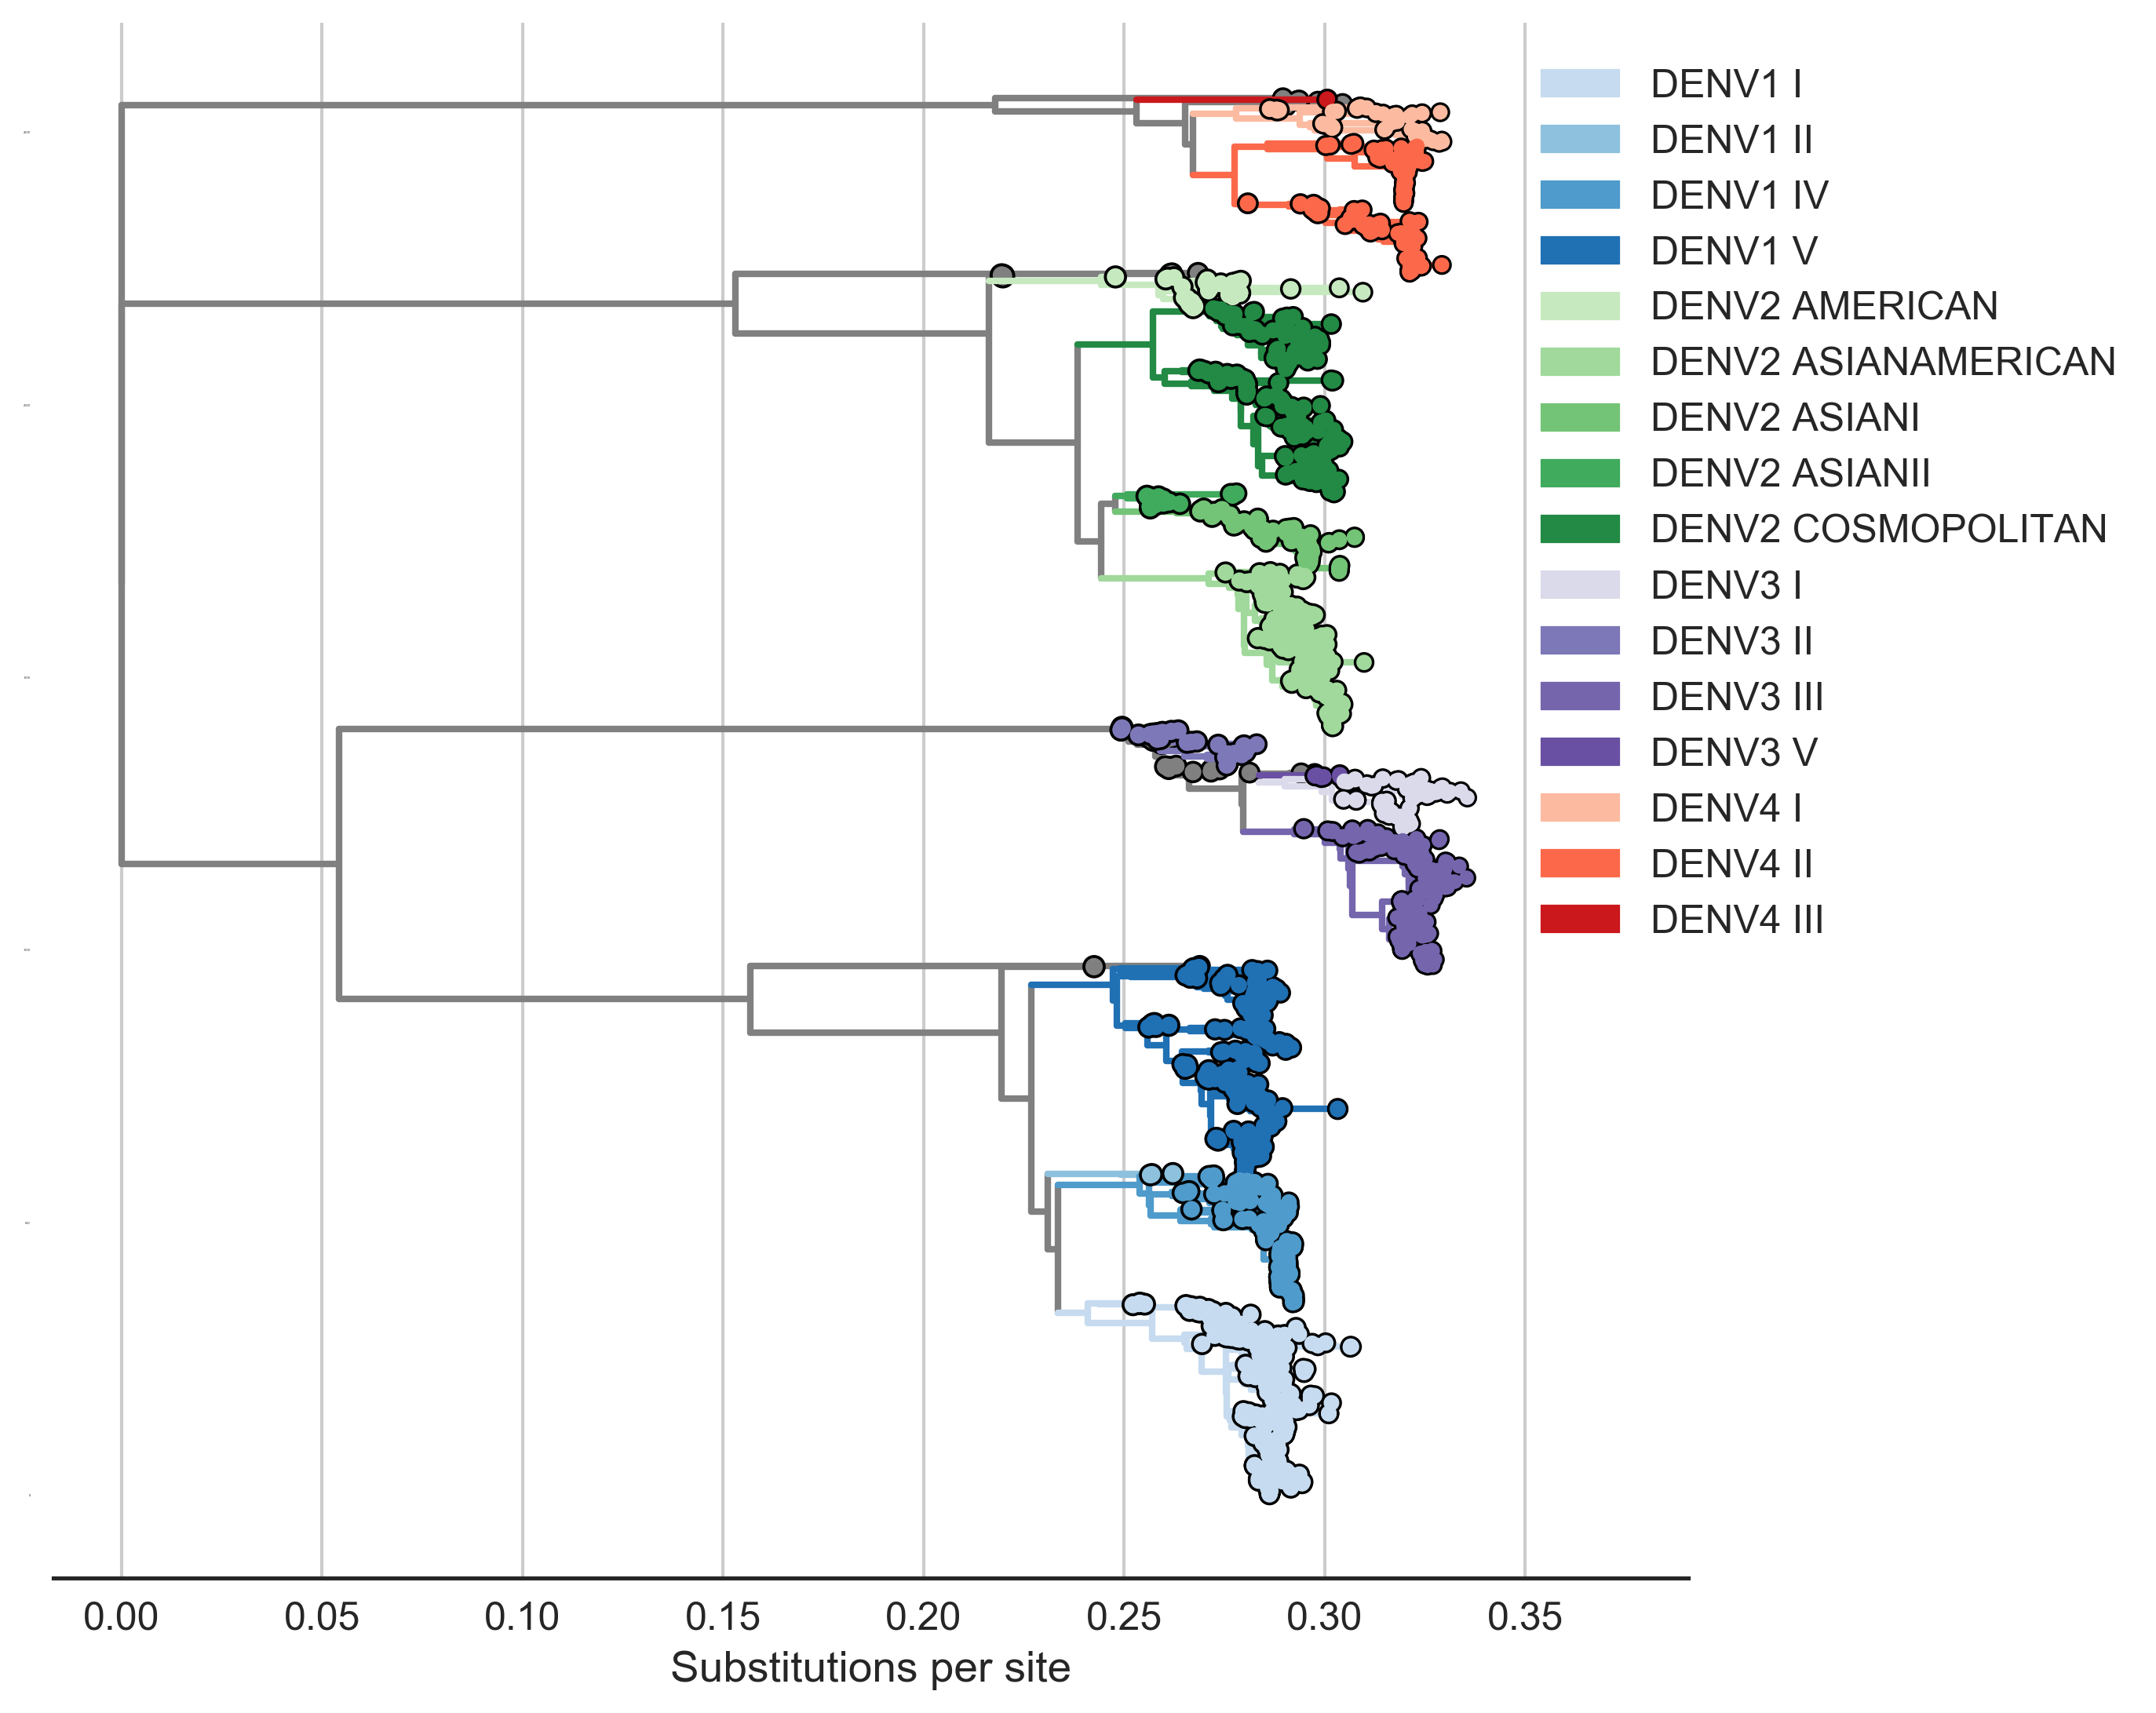
\includegraphics[width=\linewidth]{./png/genotype_tree.png}
  	\caption{\textbf{Phylogeny of dengue viral sequences.}
    Maximum likelihood phylogeny of dengue virus genomes, colored by canonical genotype assignment.
    }
  	\label{genotype_tree}
  \end{centering}
\end{figure}

One explanation for these and similar observations is that overlooked intraserotype antigenic variation contributes to these genotype-specific case outcomes and epidemic patterns.
Recent efforts to antigenically characterize diverse DENV viruses suggests that each serotype may contain antigenic heterogeneity, but the source and impact of this heterogeneity is not clear \citep{katzelnick2015dengue}.
Here, we take a phylogenetic approach to characterize the evolutionary basis for observed antigenic heterogeneity among DENV clades.
We also quantify the impact of within- and between-serotype antigenic variation on real-world DENV population dynamics.
% \end{fold}

\section{Measuring antigenic relationships between dengue viruses}
% \begin{fold}
Antigenic distance between a pair of viruses $i$ and $j$ is experimentally quantified using neutralization titer, which measures how well serum drawn after infection with virus $i$ is able to neutralize virus $j$ in vitro\citep{russell1967dengue}.
To measure the pairwise antigenic distances for a panel of diverse DENV viruses (Figure~\ref{titered_strains_tree}), Katzelnick et al. infected naive non-human primates (NHP) with each virus, drew sera at three months post-infection, and then titered this sera against a panel of test viruses \citep{katzelnick2015dengue}.
To compare patterns of cross-protection in NHP and humans, they also drew sera from 31 study participants six weeks after inoculation with a monovalent component of the NIH dengue vaccine candidate.
This sera was also titered against a broad panel of DENV viruses.
As originally reported, we find generally consistent patterns of neutralization between the NHP and human sera data; see \citep{katzelnick2015dengue} for a detailed comparison.
In total, our dataset consists of 454 NHP sera titrations spanning the breadth of DENV diversity, and 728 human sera titrations providing deep coverage of a small subset of viruses.

To standardize these measurements, we first take the log$_2$ of each value, such that one titer unit corresponds to one, two-fold drop in neutralization.
We then define antigenic distance between autologous virus-sera pairs (i.e., virus $i$ and serum $i$) as zero.
Normalized antigenic distance between $i$ and $j$ are thus calculated as $D_{ij} = \mathrm{log}_2(T_{ii}) - \mathrm{log}_2(T_{ij})$, such that a higher value of $D_{ij}$ indicates that serum $i$ is less effective at neutralizing virus $j$, implying greater antigenic distance between viruses $i$ and $j$.

The full dataset of standardized titer values is shown in Figure~\ref{titer_heatmap}.
Here, we see that homotypic virus-serum pairs are more closely related antigenically than heterotypic pairs.
However, we also observe large variance around this trend, both within and between serotypes.
This suggests that treating each serotype as antigenically uniform overlooks potentially important antigenic heterogeneity across viruses within each serotype.

\begin{figure}[h]
\begin{centering}
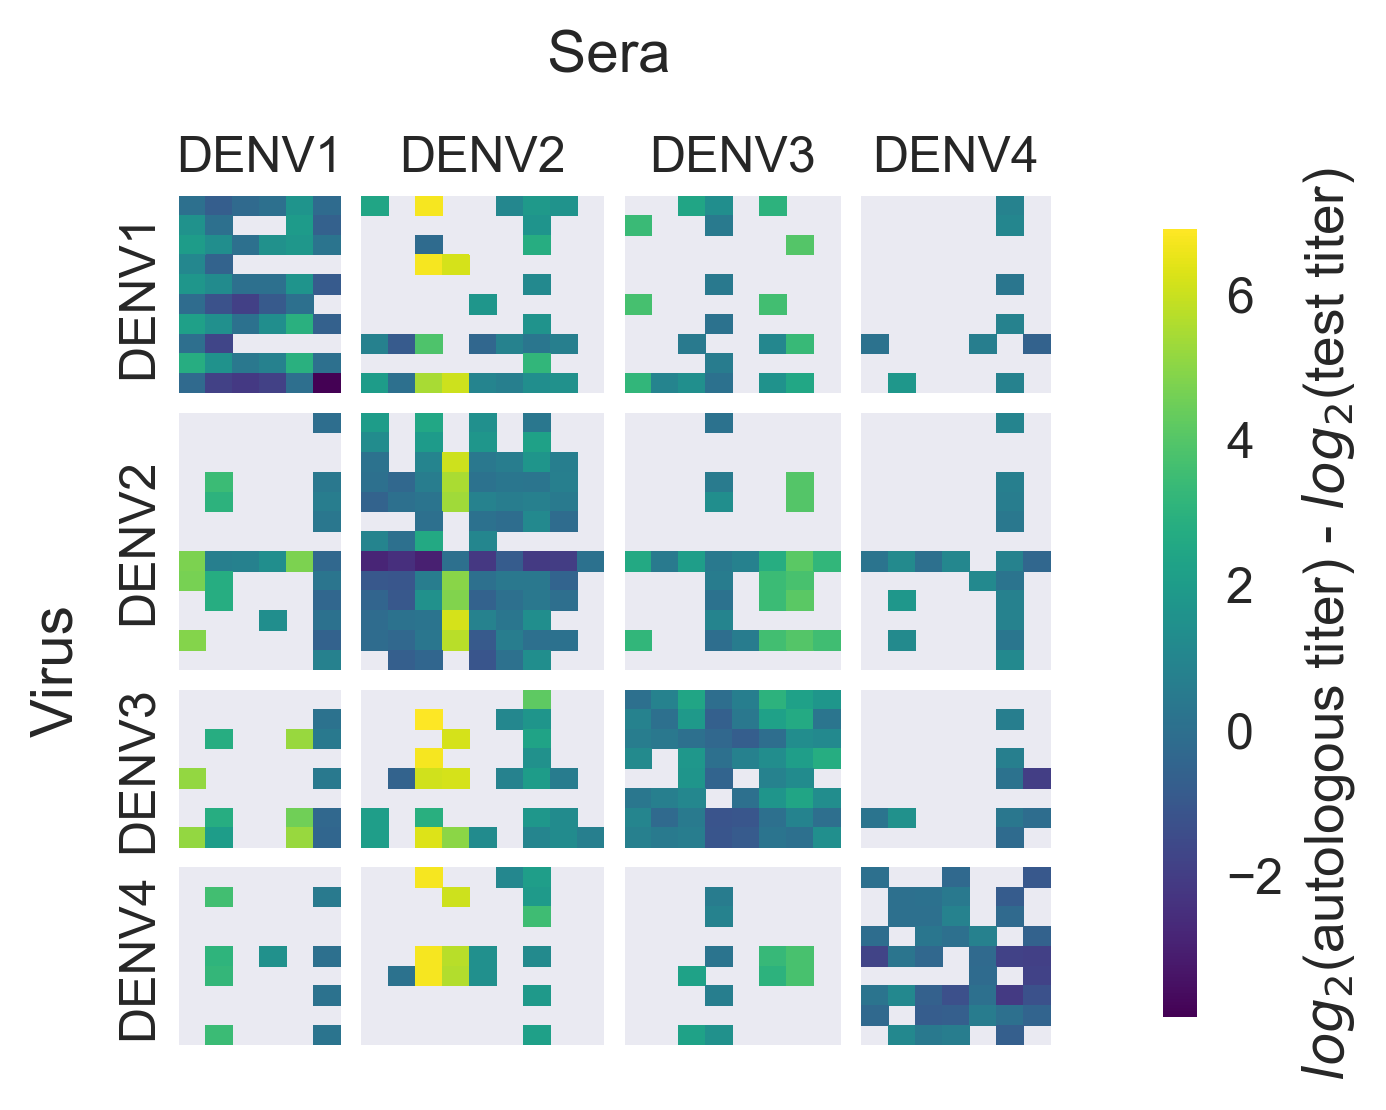
\includegraphics[width=0.65\textwidth]{./png/titer_heatmap.png}
    \caption{\textbf{Normalized antigenic distance between pairs of dengue viruses and sera.}
    Aggregated neutralization titers from Katzelnick et al. are standardized such that the distance between autologous virus-serum pairs is 0, and each titer unit corresponds to one, two-fold change in PRNT50 value.
    Light gray areas represent missing data.
    Higher values correspond to greater antigenic distance.
    }
     \label{titer_heatmap}
\end{centering}
\end{figure}
% \end{fold}

\section{Mapping dengue antigenic evolution to phylogenetic divergence}
% \begin{fold}
\begin{figure}[h]
  \begin{centering}
  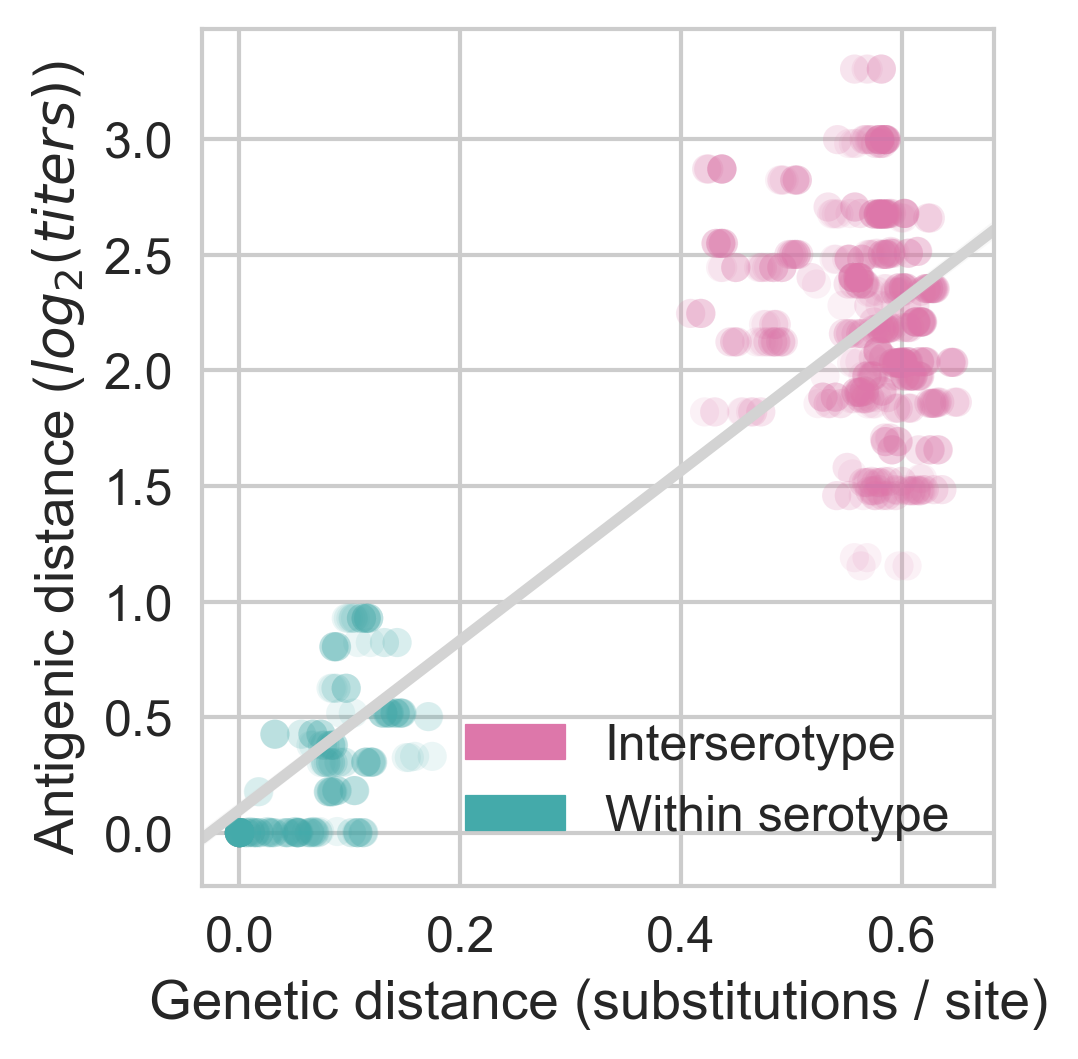
\includegraphics[width=0.6\textwidth]{./png/genetic_antigenic_distance.png}
  	\caption{\textbf{Normalized antigenic distance vs. genetic distance between pairs of dengue viruses.}
    Antigenic distances are the same as from Figure~\ref{titer_heatmap};
    genetic distances are the patristic distances between viral genomes on a maximum likelihood phylogeny.
    }
  	\label{genetic_antigenic_distance}
  \end{centering}
\end{figure}

Titer measurements are prone to noise, and there is a limited amount of available titer data.
If the antigenic heterogeneity observed in the raw data is truly the result of an underlying evolutionary process, we expect that changes in antigenic phenotype correspond to underlying changes in viral genotype.
Figure~\ref{genetic_antigenic_distance} shows the relationship between genetic and antigenic distance between each pair of viruses in our dataset.
There are two groups of comparisons --- between serotype and within serotype --- however, even within serotypes there is significant genetic diversity and a correlation between increased genetic distance and increased antigenic distance.
The relationship between genetic distance and antigenic distance is consistent within and between serotypes, where increasing genetic divergence generally corresponds to increased antigenic distance.
% \end{fold}

\section{Within-serotype antigenic evolution}
% \begin{fold}
To fully map the relationship between DENV genetic and antigenic evolution, we adapt a phylogeny-based model originally developed for influenza \citep{neher2016prediction}.
Conceptually, this model predicts titer values through three steps.
First, we build a phylogeny of dengue virus sequences to establish the genetic relationships between viruses (Figures~\ref{genotype_tree}, \ref{sequence_distribution}).
Next, we infer how much antigenic change has occurred along each branch of the phylogeny by mapping titer changes to individual branches.
This assigns each branch $b$ an antigenic distance $d_b$.
With this in hand, we estimate the antigenic distance between all pairs of viruses by tracing the path between them in the phylogeny, summing branch-specific distances $d_b$ as we go (Methods, Eq.~\ref{eq_predicted_titers}).

To learn these values of $d_b$, we first split our dataset into training (random 90\% of measurements) and test data (the remaining 10\% of values).
We take the training data and fit $d_b$ for each branch in the tree, subject to regularization as follows (also detailed in Methods, Eq.~\ref{eq_cost_fn}).
Parsimoniously, we expect that antigenic change is more likely to occur through larger changes on a few branches than through small changes on many branches; correspondingly, our prior expectation of values of $d_b$ is exponentially distributed such that most values of $d_b = 0$.
This is analogous to lasso regression to identify a few parameters with positive weights and set other parameters to 0.
Additionally, some viruses have greater binding avidity, and some sera are more potent than others (Figure~\ref{titer_asymmetry}); these `row' and `column' effects, respectively, are normally distributed and are taken into account when estimating titers.
The model uses convex optimization to learn the values of $d_b$ that minimize the sum of squared errors (SSE) between observed and predicted titers in the training data.

\begin{figure}[h]
  \begin{centering}
    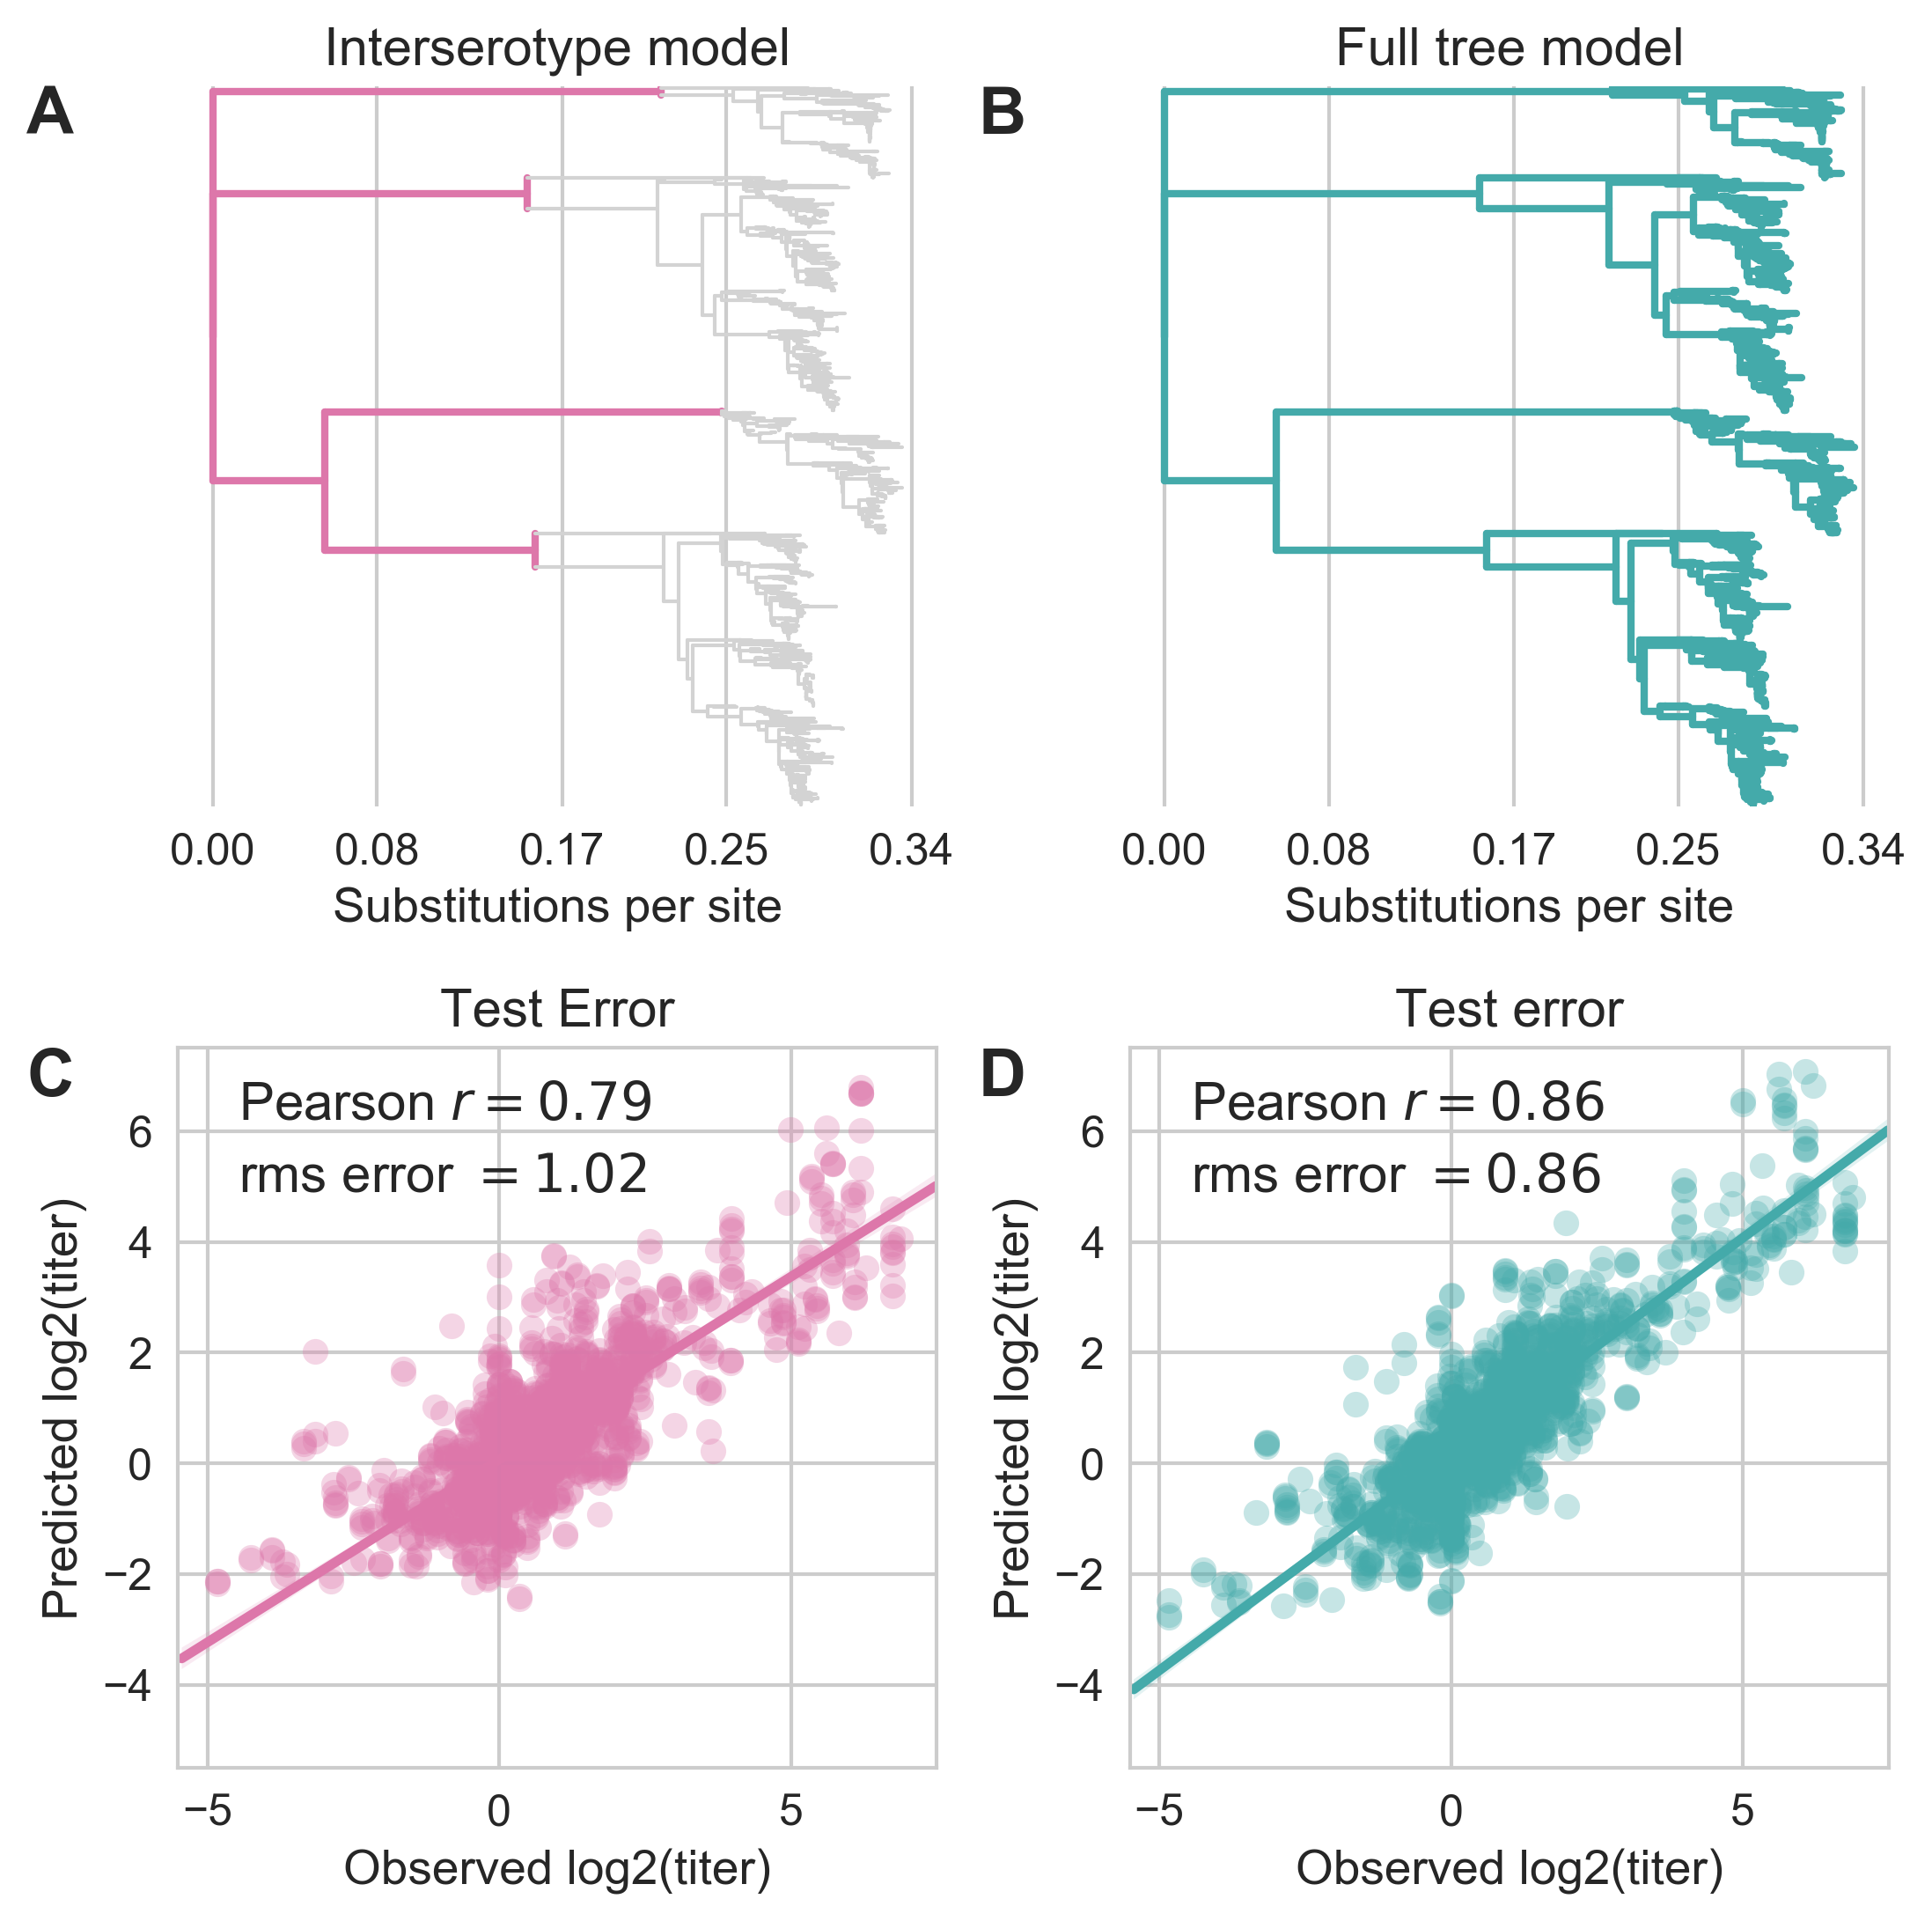
\includegraphics[width=0.8\textwidth]{./png/titer_model_performance.png}
        \caption{\textbf{Titer model formulations and performance.}
        \textbf{A} The `interserotype model' only allows branches that lie between serotypes to contribute to antigenic evolution.
        All other branches are assigned $d_b = 0$.
        \textbf{B} The `full tree model' allows any branch in the phylogeny to contribute to antigenic evolution ($d_b >= 0$).
        \textbf{C,D} Predictive performance of each model on the test dataset (aggregated from 10-fold cross-validation).
        Shading represents the 95\% confidence interval.
        }
         \label{titer_model_performance}
  \end{centering}
\end{figure}

This model formulation is an effective tool for estimating antigenic relationships between viruses based on their relative positions in the phylogeny.
We can use variations of this model to explicitly test whether the observed antigenic phenotypes are better explained by the hypothesis that dengue serotypes are antigenically uniform (`interserotype model'), or by the hypothesis that serotypes are antigenically diverse (`full tree model').
In the interserotype model, we set $d_b = 0$ for all branches in the tree that do not lie between serotypes (Figure~\ref{titer_model_performance}A).
Alternatively, the `full tree model' allows any branch in the phylogeny to contribute to antigenic evolution (Figure~\ref{titer_model_performance}B).
For each model, we learn model parameters from the training data, and then use those parameters to predict test data values.
We assess model performance by comparing the predicted test titer values to the actual values.
Model performance indicates how well the hypothesis embedded in the model explains the observed data.

We find that serotype-level characterization alone explains observed antigenic phenotypes to a reasonable degree.
On average, this interserotype model predicts titers within 1.02 log$_2$ titer units of the true value (root mean squared error, RMSE), and explains 62\% of the observed variation in neutralization titers overall (Figure~\ref{titer_model_performance}).

However, we find that accounting for within-serotype antigenic evolution substantially improves our ability to explain dengue antigenic phenotypes.
The full tree model is able to predict test titers within 0.86 log$_2$ titer units of the true value (RMSE approaching the level of error intrinsic to the assay), and explains 74\% of the observed variation in neutralization titers overall (Figure~\ref{titer_model_performance}).
Importantly, all reported error metrics refer to performance on test data, so this difference in model performance is not due to the number of free parameters.
The full tree model performance is comparable to the model error from a cartography-based characterization of the same dataset (RMSE 0.65--0.8 log$_2$ titer units), and to the error observed when this model was used to characterize an influenza dataset (RMSE of 0.5 log$_2$ titer units) \citep{katzelnick2015dengue,neher2016prediction}.
From this, we conclude that there is antigenic evolution within each serotype of DENV, and that this is driven by underlying genetic divergence.

Collapsing putatively antigenically uniform clades, we observe at least 12 distinct antigenic phenotypes of DENV (Figure~\ref{antigenic_tree}) and reject the null hypothesis that all DENV viruses within a serotype are antigenically uniform.
The titer dataset spans the breadth of canonical DENV genotypes, but in most cases lacks the resolution to detect within-genotype antigenic diversity.
We thus expect that these results represent a lower-bound on the true extent of DENV intraserotype antigenic diversity.

\begin{figure}[h]
  \begin{centering}
    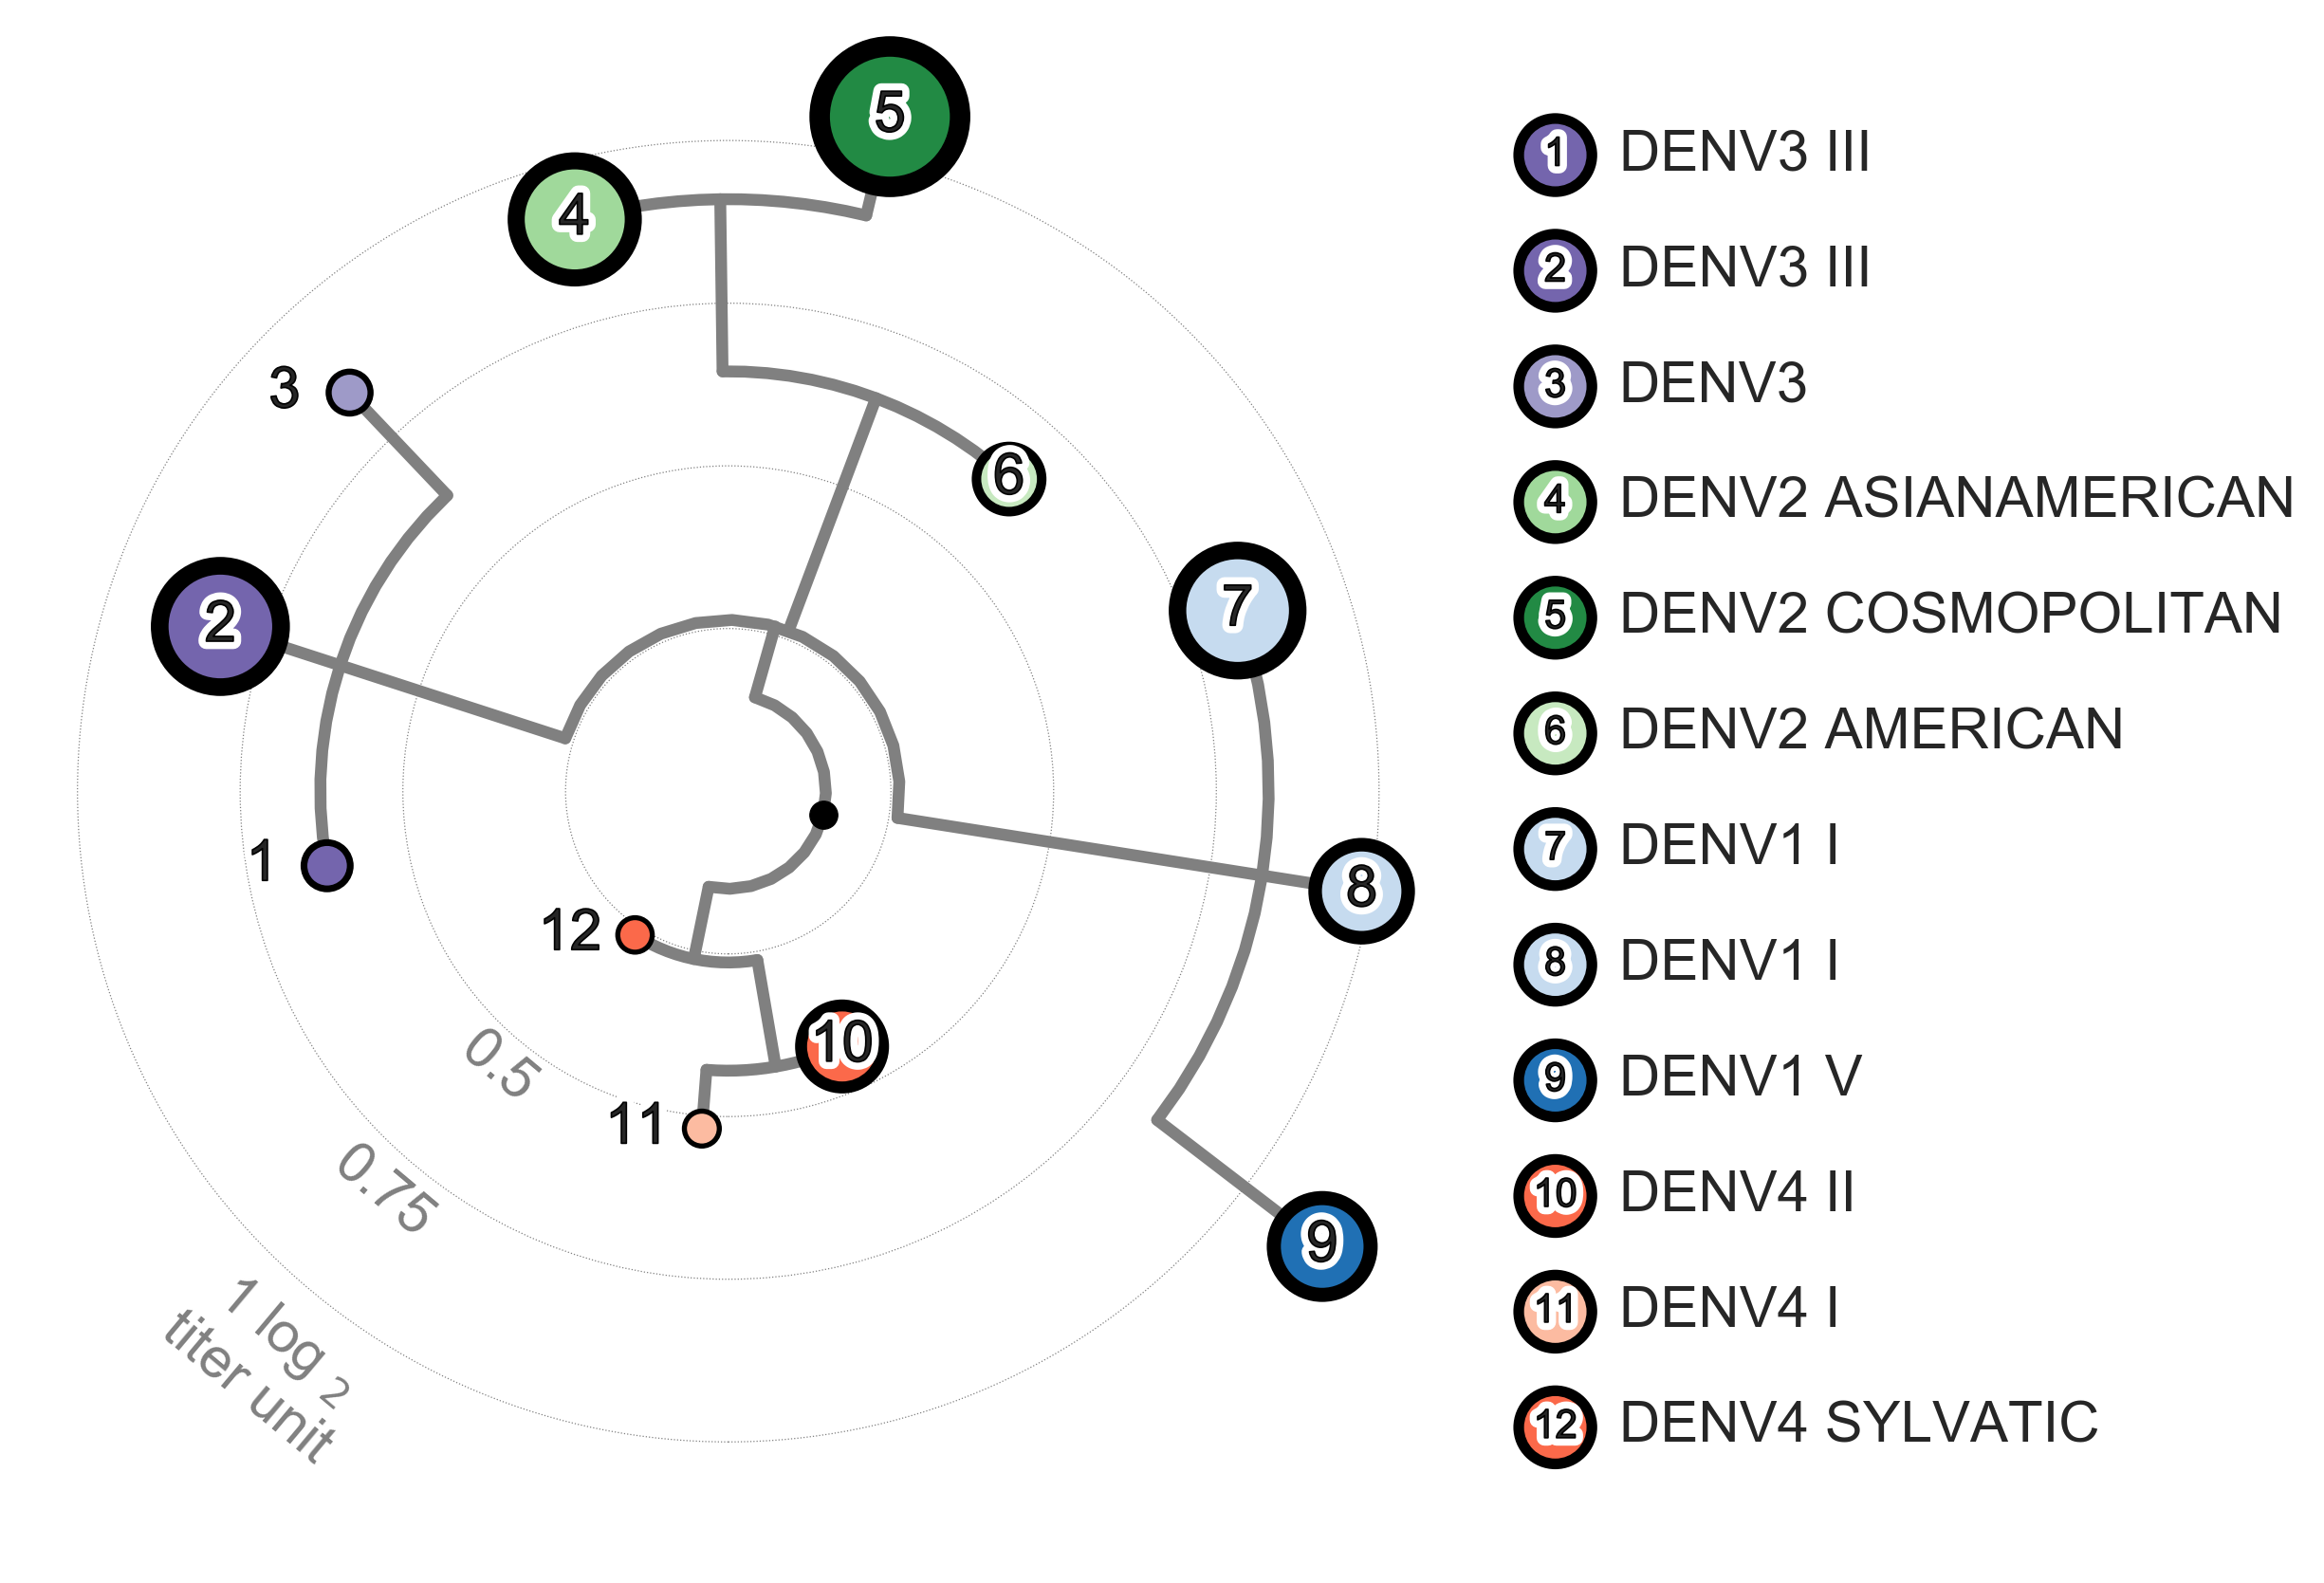
\includegraphics[width=\linewidth]{./png/antigenic_tree.png}
    \caption{\textbf{Tree of dengue antigenic phenotypes.}
    We infer the topology from a maximum likelihood phylogeny of DENV genomes.
    Branch lengths are scaled to reflect $d_b$, the relative contributions of each branch to antigenic divergence, as inferred by the `full tree' model of DENV evolution.
    Antigenically uniform clades are collapsed, and node diameter reflects the size of the collapsed clade.
    Figure~\ref{antigenic_tree_supplement} offers an additional view of the same topology.
    }
     \label{antigenic_tree}
  \end{centering}
\end{figure}
% \end{fold}

\section{Discussion}
% \begin{fold}
We show that mapping antigenic change to individual branches and interpolating across the DENV phylogeny is able to explain a large majority of the observed variation in antigenic phenotypes, as measured by neutralization titers.
This demonstrates that DENV antigenic divergence is closely coupled to genetic divergence.
We also find that accounting for within-serotype antigenic evolution is necessary to explain the observed variation in antigenic phenotypes.
This supports and expands upon previous reports \citep{katzelnick2015dengue} that the null hypothesis of antigenically uniform serotypes is inconsistent with observed patterns of cross-protection and susceptibility.
We observe at least 12 distinct antigenic phenotypes that are both genetically and antigenically distinct.
Analysis of the recent CYD-TDV vaccine trial shows different vaccine efficacy against genotypes I and II of DENV4 \citep{juraska2018viral}; the antigenic distance between these two genotypes is comparable to the antigenic distance separating each of the 12 antigenic phenotypes we report (Figures~\ref{antigenic_tree}, \ref{genotype_dTiter_heatmap}).
This suggests that these phenotypes may be sufficiently distinct to have important impacts on secondary case outcomes and vaccine efficacy.

Overall, we expect that these antigenic phenotypes represent a lower-bound on the extent, magnitude, and nature of antigenic heterogeneity with DENV.
Our current titer dataset spans the breadth of DENV diversity, but due to small sample size, it lacks the resolution to detect most sub-genotype antigenic variation or to identify which specific mutations correspond to changes in antigenic phenotype.
The appearance of the deep antigenic divergence of the four serotypes, and the more recent antigenic divergences within each serotype, suggest that DENV antigenic evolution is likely an ongoing, though gradual, process.
We therefore expect that future studies with richer datasets will find additional antigenic variation within each genotype.
This dataset also contains many left-censored titer values, where we know two viruses are at least $T$ titer units apart, but do not know exactly how far apart.
If we knew the true value of these censored titers, many of them would indicate larger antigenic distances than the reported values, $T$, which are used to train the model.
Thus, it is likely that our model systematically underestimates the magnitude of titer distances.
Finally, antibody neutralization and escape (as measured by PRNT titers) is only one component of the immune response to DENV.
Although analysis of a longitudinal cohort study shows that these neutralization titers correlate with protection from severe secondary infection, it is unclear how PRNT titers correspond to antibody-dependent enhancement \citep{katzelnick2016neutralizing}.
It is also important to note that DENV case outcomes are partially mediated by interactions with innate and T-cell immunity, the effects of which are not captured in neutralization titers \citep{green2014innate}.
Overall, while richer datasets and the development of more holistic assays will be required in order to fully characterize the extent of DENV antigenic diversity, it is clear that the four-serotype model is insufficient to explain DENV antigenic evolution.
% \end{fold}

\section{Methods}
% \begin{fold}
\subsection*{Sequence Data}
We downloaded all dengue virus sequences available from the Los Alamos National Lab Hemorrhagic Fever Virus Database as of March 7, 2018, that contained the full coding sequence of E (total N=12,645) \citep{kuiken2011lanl}.
We discarded sequences which were putative recombinants, duplicates, lab strains, or which lacked an annotated sampling location and/or sampling date.
We then randomly subsampled up to 8 viruses per region, per month, preferentially including records with available titer data and longer sequences.
Our final dataset consists of 2,563 viral sequences (Figure~\ref{sequence_distribution}).
We used the annotated reference dataset from \citep{pyke2016highly} to assign sequences to canonical genotypes.

\subsection*{Titer Data}

Antigenic distance between pairs of viruses $i$ and $j$ is experimentally measured using a neutralization titer, which measures how well serum drawn after infection with virus $i$ is able to neutralize virus $j$ in vitro \citep{russell1967dengue}.
Briefly, two-fold serial dilutions of serum $i$ are incubated with a fixed concentration of virus $j$.
Titers represent the lowest serum concentration able to neutralize $50\%$ of virus, and are reported as the inverse dilution.
We used two publicly available plaque reduction neutralization titer (PRNT50) datasets generated by Katzelnick et al. in \citep{katzelnick2015dengue}.
The primary dataset was generated by infecting each of 36 non-human primates with a unique strain of DENV.
NHP sera was drawn after 12 weeks and titered against the panel of DENV viruses.
The secondary dataset was generated by vaccinating 31 human trial participants with a monovalent component of the NIH DENV vaccine.
Sera was drawn after 6 weeks and titered against the same panel of DENV viruses.
As discussed in Katzelnick et al., these two datasets show similar patterns of antigenic relationships between DENV viruses.
In total, our dataset includes 47 virus strains, 36 serum strains, and 1182 measurements.

\subsection*{Titer Model}
We compute standardized antigenic distance between virus $i$ and serum $j$ (denoted $D_{ij}$) from measured titers relative to autologous titers (denoted $T_{ii}$ and $T_{ij}$, respectively), such that
\begin{equation}
  \label{eq_titer_norm}
D_{ij} = \mathrm{log}_2(T_{ii}) - \mathrm{log}_2(T_{ij})
\end{equation}
To predict unmeasured titers, we employ the `tree model' from Neher et al. and implemented in Nextstrain, which assumes that antigenic evolution is driven by underlying genetic evolution \citep{hadfield2017nextstrain,neher2016prediction}.
We use RAxML version 8.2.11 and a GTRCAT nucleotide substitution model to build a maximum likelihood phylogeny of dengue viral genome sequences \citep{stamatakis2014raxml}.
Observed titer drops are mapped to branches in the viral phylogeny after correcting for overall virus avidity, $v_i$, and serum potency, $p_j$ (`row' and `column' effects, respectively):
\begin{equation}
  \label{eq_predicted_titers}
\hat{D}_{ij} \approx D_{ij} = \sum_{b \in path(i,j)} d_b + v_i + p_j
\end{equation}
where $d_b$ is the titer drop assigned to each branch, $b$, in the phylogeny.
We randomly withhold 10\% of titer measurements as a test set.
We use the remaining 90\% of titer measurements as a training set to learn values for virus avidity, serum potency, and branch effects.
As in Neher et al., we formulate this as a convex optimization problem and solve for these parameter values to minimize the cost function:
\begin{equation}
  \label{eq_cost_fn}
C = \sum_{i,j} (\hat{D}_{ij} - D_{ij})^2 + \lambda \sum_{b} d_b + \gamma \sum_{i} v_i^2 + \delta \sum_{j} p_j^2
\end{equation}
Respectively, these terms represent the squared training error; an L1 regularization term on branch effects, such that most values of $d_b = 0$; and L2 regularization terms on virus avidities and serum potencies, such that they are normally distributed.
These parameter values are then used to predict the antigenic distance between all pairs of viruses, $i$ and $j$, in the phylogeny.
We assess performance by comparing predicted to known titer values in our test data set, and present test error (aggregated from 10-fold cross-validation) throughout the manuscript.

% \end{fold}
% \end{fold}

% ========== Dengue Population Immunity Chapter
\chapter{Human population immunity and dengue virus clade dynamics}
% \begin{fold}
\section{Antigenic novelty and serotype turnover}
% \begin{fold}
From the titer model, we observe strong evidence that homotypic genotypes of DENV vary in their ability to escape antibody neutralization (Figures~\ref{titer_model_performance}, \ref{genotype_dTiter_heatmap}).
However, antibody neutralization is only one of many factors that shape epidemic patterns.
We investigate whether the observed antigenic diversity influences dengue population dynamics in the real world.
The size of the viral population (i.e., prevalence, commonly analyzed using SIR models as reviewed in \citep{lourencco2018challenges}) is determined by many complex factors, and reliable values for population prevalence are largely unavailable.
Contrastingly, the composition of the viral population (i.e., the relative frequency of each viral clade currently circulating) can be estimated over time by examining historical sequence data \citep{lee2018deep,neher2016prediction}, and is primarily driven by viral fitness \citep{bedford2011strength}.
In meaningfully antigenically diverse viral populations, antigenic novelty (relative to standing population immunity) contributes to viral fitness: as a given virus $i$ circulates in a population, the proportion of the population that is susceptible to infection with $i$--and other viruses antigenically similar to $i$--decreases over time as more people acquire immunity \citep{bedford2012canalization, luksza2014predictive}.
Antigenically novel viruses that are able to escape this population immunity are better able to infect hosts and sustain transmission chains, making them fitter than the previously circulating viruses \citep{zhang2005clade, bedford2012canalization}.
Thus, if antigenic novelty constitutes a fitness advantage for DENV, then we would expect greater antigenic distance from recently circulating viruses to correlate with higher growth rates.

\begin{figure}[h]
  \begin{centering}
    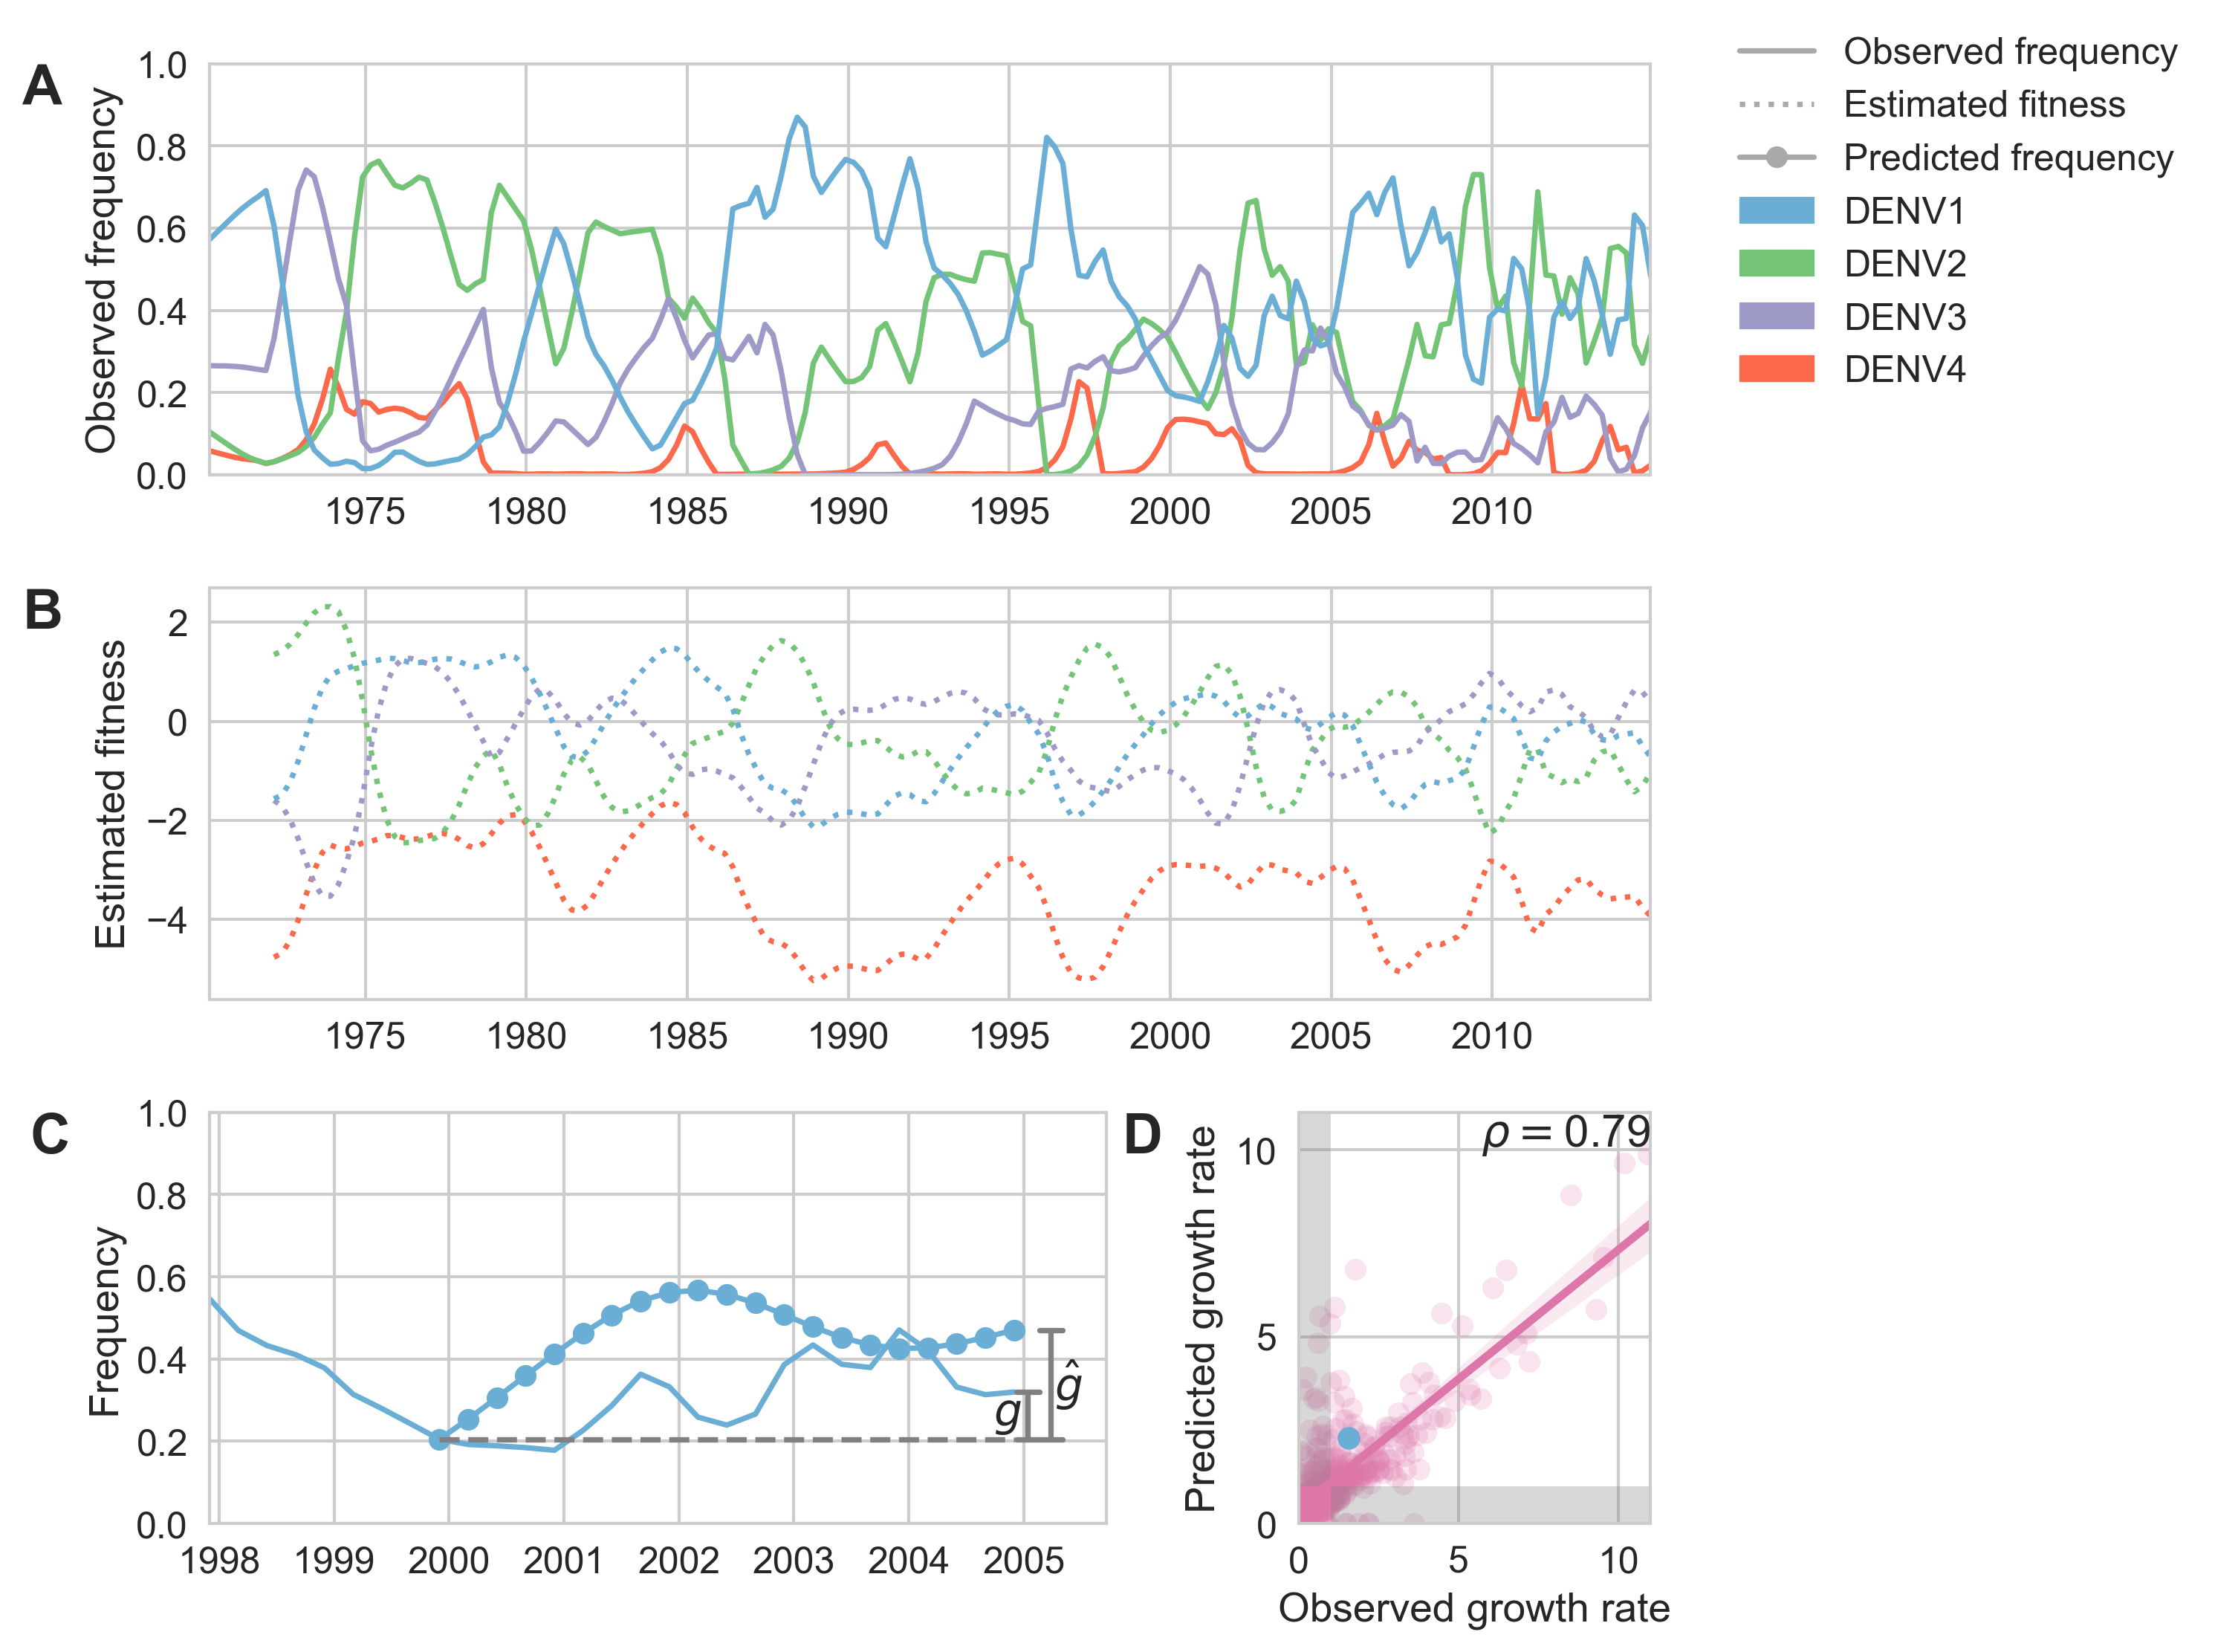
\includegraphics[width=\linewidth]{./png/serotype_fitness_model.png}
  	\caption{\textbf{Antigenic novelty predicts serotype success.}
    \textbf{A} The relative frequency of each serotype, $x_i$, in Southeast Asia is estimated every three months based on available sequence data.
    \textbf{B} We calculate antigenic fitness for each serotype over time as its frequency-weighted antigenic distance from recently circulating viruses.
    We then add this to a time-invariant intrinsic fitness value to calculate total fitness (shown here, arbitrary units).
    \textbf{C} illustrates how the model predicts clade growth rates.
    At each timepoint $t$, we blind the model to all empirical data from timepoints later than $t$ and predict each serotype's future trajectory based on its initial frequency, time-invariant intrinsic fitness, and antigenic fitness at time $t$ (Methods, Eq.~\ref{eq_predict_frequency}).
    We predict forward in three-month increments for a total prediction period of $dt = 5$ years.
    At each increment, we use the predicted stepwise frequency change to adjust our estimates of antigenic fitness on a rolling basis (Methods, Eq.~\ref{eq_compounding_immunity}).
    Predicted growth rates are calculated as $\hat{g} = \frac{\hat{x_i}(t+dt)}{x_i(t)}$ and compared to empirically observed growth rates, $g = \frac{x_i(t+dt)}{x_i(t)}$ in \textbf{D}.
    The example illustrated in \textbf{C} is also shown in \textbf{D} as the blue point.
    Serotype growth versus decline is accurate (i.e., the predicted and actual growth rates are both $>1$ or both $<1$, all points outside the gray area) for 80\% of predictions.
    }
  	\label{serotype_fitness_model}
  \end{centering}
\end{figure}

To test this hypothesis, we examine the composition of the dengue virus population in Southeast Asia from 1970 to 2015.
We estimate the relative population frequency of each DENV serotype at three month intervals, $x_i(t)$ (Figure~\ref{serotype_fitness_model}A), based on available sequence data (Methods, Eq.~\ref{eq_estimate_frequency}).

Fitter virus clades increase in frequency over time, such that $x_i(t+dt) > x_i(t)$.
It follows that these clades have a growth rate--defined as the fold-change in frequency over time--greater than one: $\frac{x_i(t+dt)}{x_i(t)} > 1$.
To isolate the extent to which antigenic fitness contributes to clade success and decline, we extend work by {\L}uksza and L\"assig* \citep{luksza2014predictive} to build a simple model that attempts to predict clade growth rates based on two variables: the antigenic fitness of the clade at time $t$, and a time-invariant free parameter representing the intrinsic fitness of the serotype the clade belongs to.
We estimate the antigenic fitness of clade $i$ at time $t$ as a function of its antigenic distance from each viral clade $j$ that has circulated in the same population over the previous two years, weighted by the relative frequency of $j$ and adjusted for waning population immunity (Figure~\ref{serotype_fitness_model}B; Methods, Eq.~\ref{eq_waning_immunity}).
Growth rates are estimated based on a five year sliding window (Figure~\ref{serotype_fitness_model}C).

This simple model explains 62\% of the observed variation in serotype growth rates, and predicts serotype growth vs decline correctly for 80\% of predictions (Figure~\ref{serotype_fitness_model}D).
This strongly suggests that antigenic fitness is a major driver of serotype population dynamics.
This also demonstrates that this model captures key components of dengue population dynamics; examining the formulation of this model in more detail can yield insights into how antigenic relationships influence DENV population composition.
The fitness model includes eight free parameters that are optimized such that the model most accurately reproduces the observed fluctuations in DENV population composition (reduction in prediction error relative to a null model, see Methods).
We find that serotype fluctuations are most consistent with a model wherein population immunity wanes linearly over time, with the probability of protection dropping by about 48\% per year for the first two years after primary infection.
We also find that these dynamics are best explained by intrinsic fitness that moderately varies by by serotype (Table~\ref{parameter_values}).
% \end{fold}

\section{Antigenic novelty and genotype success}
% \begin{fold}
To estimate how well antigenic fitness predicts genotype dynamics, we used the same model to predict genotype success and decline.
As before, fitness of genotype $i$ is based on the intrinsic fitness of the serotype $i$ belongs to, and the antigenic distance between $i$ and each other genotype, $j$, that has recently circulated (Figure~\ref{genotype_fitness}B).
Importantly, we can calculate antigenic distance between $i$ and $j$ at the serotype level (i.e., the antigenic distances computed from the `interserotype model' as illustrated in Figure~\ref{titer_model_performance}A) or at the genotype level (i.e., the antigenic distances computed by the `full tree model' as illustrated in Figure~\ref{titer_model_performance}B, which incorporates the observed within-serotype heterogeneity).
If within-serotype antigenic heterogeneity contributes to genotype fitness, then we would expect estimates of antigenic fitness based on the `full tree model' to better predict genotype growth rates.

We find that antigenic fitness contributes to genotype turnover, although it explains less of the observed variation than for serotypes.
When antigenic distance is estimated from the `interserotype model', we find that our model of antigenic fitness explains approximately 31\% of the observed variation in genotype growth rates, and correctly predicts genotype growth vs. decline 68\% of the time (Figure~\ref{genotype_fitness}C).
Perhaps surprisingly, more precise estimates of antigenic distance between genotypes from the `full tree model' does not improve our predictions of genotype success ($R^2 = 0.28$, 70\% accuracy; Figure~\ref{genotype_fitness}D).
This suggests that although we find strong evidence that genotypes vary in their ability to escape neutralizing antibodies (Figures~\ref{titer_model_performance}, \ref{genotype_dTiter_heatmap}), these differences are subtle enough that they do not impact broad-scale regional dynamics over time.

\begin{figure}[h]
  \begin{centering}
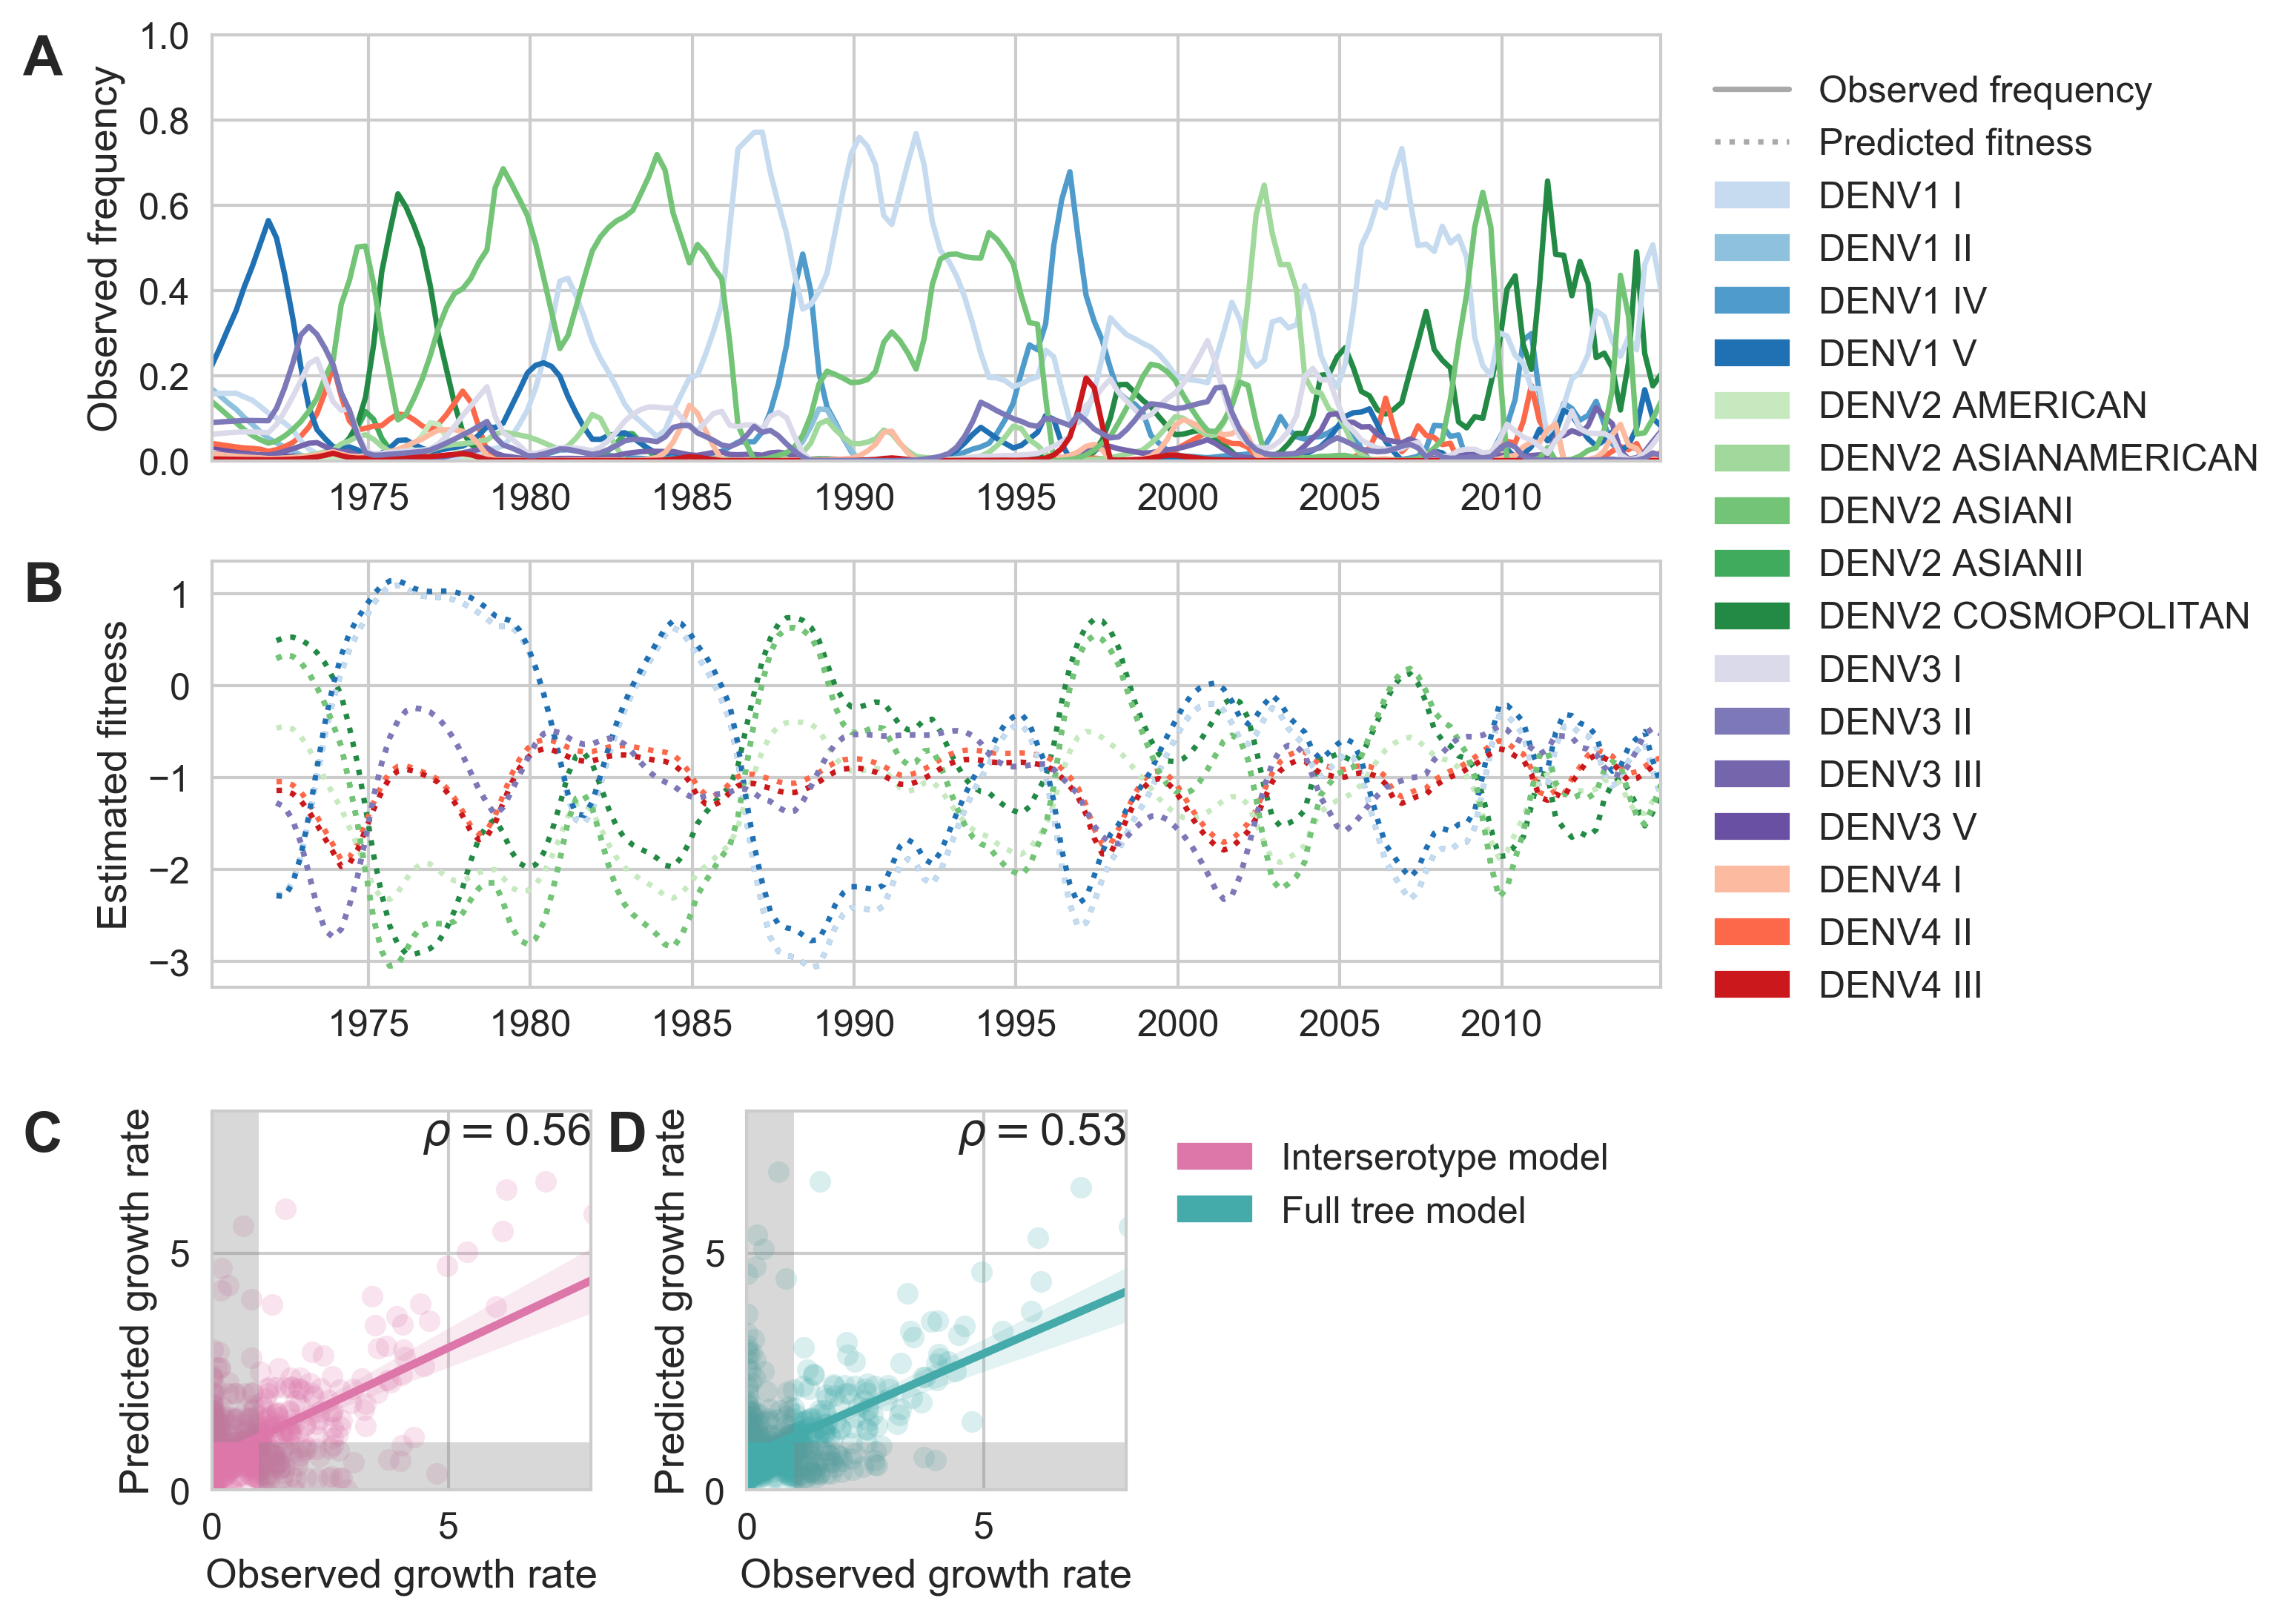
\includegraphics[width=\linewidth]{./png/genotype-fitness.png}
    \caption{\textbf{Relative frequencies and fitness of dengue genotypes, 1970-2015.}
    \textbf{A} Relative frequencies of each canonical dengue genotype across Southeast Asia, estimated from available sequence data.
    \textbf{B} Antigenic fitness is calculated for each genotype as its frequency-weighted antigenic distance from recently circulating genotypes.
    We then add this to a time-invariant, serotype-specific intrinsic fitness value to calculate total fitness (shown here, arbitrary units).
    We assess antigenic distance using either the `full tree model' or the `interserotype model' of antigenic relationships (Figure~\ref{titer_model_performance}).
    In this panel, we show total fitness over time, incorporating estimates of antigenic fitness derived from the `full tree' model.
    \textbf{C, D}  Fitness estimates were used to predict clade growth rates over 5 years, compounding immunity every three months based on predicted frequency changes (Methods Eq.~\ref{eq_compounding_immunity}).
    Here, we compare observed vs predicted growth rates for both formulations of the fitness model (using fitness derived from either the `interserotype' or `full tree' model estimates of antigenic distance).
    Growth versus decline was accurate (predicted and actual growth rates both $> 1$ or both $< 1$, points outside the gray shaded area) for 68\% -- 70\% of predictions, respectively.
}
     \label{genotype_fitness}
   \end{centering}
\end{figure}

% \end{fold}

\section{Discussion}
% \begin{fold}
We use these inferred antigenic relationships to directly quantify the impact of antigenic fitness on DENV population composition.
To do so, we measure serotype frequencies across Southeast Asia over time and construct a model to estimate how they will fluctuate (Methods, Eq.~\ref{eq_population_immunity}--\ref{eq_delta_sse}).
This model places a fitness value on each serotype that derives from a constant intrinsic component alongside a time-dependent antigenic component.
Antigenic fitness declines with population immunity, which is accumulated via the recent circulation of antigenically similar viruses.
We find that antigenic fitness is able to explain most of the observed variation in serotype growth and decline (Figure~\ref{serotype_fitness_model}).
This demonstrates that antigenic fitness is a strong determinant of DENV serotype dynamics in a real-world, hyperendemic population.

We similarly use this model to quantify the effect of within-serotype antigenic variation on the success and decline of canonical DENV genotypes (Figure~\ref{genotype_fitness}).
As above, genotype antigenic fitness declines with population immunity.
Here, we estimate population immunity based on antigenic distance from recently circulating genotypes, using distances derived from the `interserotype model' or the `full tree model' of DENV antigenic evolution.
We then directly compare how strongly these coarser serotype-level versus specific genotype-level antigenic relationships impact DENV population dynamics.
Overall, we find that antigenic fitness explains a moderate portion of the observed variation in genotype growth and decline.
Surprisingly, however, we find that incorporating within-serotype antigenic differences does not improve our predictions (Figure~\ref{genotype_fitness}C,D).
This suggests that although genotypes are antigenically diverse, these differences do not appear to influence large-scale regional dynamics over time.

However, this observation is subject to caveats imposed by the the available data and model assumptions.
Our estimates of antigenic fitness are informed by the antigenic distances inferred by the titer tree model; thus, as above, we are unable to account for nuanced antigenic differences between sub-genotype clades of DENV due to limited titer data.
We estimate DENV population composition over time based on available sequence data, pooled across all of Southeast Asia (Methods, Eq.~\ref{eq_estimate_frequency}).
As the vast majority of cases of DENV are asymptomatic, sequenced viruses likely represent a biased sample of more severe cases from urban centers where patients are more likely to seek and access care.
We also assume that Southeast Asia represents a closed viral population with homogeneous mixing.
However, increasing globalization likely results in some amount of viral importation that is not accounted for in this model \citep{allicock2012phylogeography}.
Finally, although Southeast Asia experiences hyperendemic DENV circulation, the majority of DENV transmissions are hyper-local \citep{salje2017dengue}, and viral populations across this broad region may not mix homogeneously each season.
Thus, it is possible that these sub-serotype antigenic differences impact finer-scale population dynamics, but we lack the requisite data to examine this hypothesis.
% \end{fold}

\section{Methods}
% \begin{fold}
\subsection*{Empirical Clade Frequencies}
As discussed in Neher et al and Lee et al, we estimate empirical clade frequencies from 1970 to present based on observed relative abundance of each clade in the `slice' of the phylogeny corresponding to each quarterly timepoint \citep{lee2018deep,neher2016prediction}.

Briefly, the frequency trajectory of each clade in the phylogeny is modeled according to a Brownian motion diffusion process discretized to three-month intervals.
Relative to a simple Brownian motion, the expectation includes an `inertia' term that adds velocity to the diffusion and the variance includes a term $x(1-x)$ to scale variance according to frequency following a Wright-Fisher population genetic process.
This results in the following diffusion process:
\begin{equation}
  \label{eq_estimate_frequency}
x(t+dt) = \mathcal{N}\left(x(t) + \epsilon dx, \; dt \sigma^2 x(t) (1-x(t))\right)
\end{equation}

with `volatility' parameter $\sigma^2$.
The term $dx$ is the increment in the previous timestep, so that $dx = x(t) - x(t-dt)$.
We used $\epsilon = 0.7$ and $\sigma = 2.0$ to maximize fit to empirical trajectory behavior.

We also include an Bernoulli observation model for clade presence / absence among sampled viruses at timestep $t$.
This observation model follows
\begin{equation}
f(x,t) = \Pi_{v \in V} x(t) \; \Pi_{v \notin V} (1-x(t))
\end{equation}
where $v \in V$ represents the set of viruses that belong to the clade and $v \notin V$ represents the set of viruses that do not belong to the clade.
Each frequency trajectory is estimated by simultaneously maximizing the likelihood of the process model and the likelihood of the observation model via adjusting frequency trajectory $\vec{x} = (x_1, ... x_n)$.

\subsection*{Population Immunity}
For antigenically diverse pathogens, antigenic novelty represents a fitness advantage \citep{lipsitch2007patterns}.
This means that viruses that are antigenically distinct from previously-circulating viruses are able to access more susceptible hosts, allowing the antigenically novel lineage to expand.
We adapt a simple deterministic model from {\L}uksza and L\"assig to directly quantify dengue antigenic novelty and its impact on viral fitness \citep{luksza2014predictive}.
We quantify population immunity to virus $i$ at time $t$, $P_i(t)$, as a function of which clades have recently circulated in the past $N$ years, and how antigenically similar each of these clades is to virus $i$:
\begin{equation}
  \label{eq_population_immunity}
P_i(t) = \sum_{n=1}^{n=N} \left(w(n)  \sum_{j} \Big( x_j(t-n) \, C( D_{ij}) \Big) \right)
\end{equation}
Where $D_{ij}$ is the antigenic distance between $i$ and each non-overlapping clade $j$, $n$ is the number of years since exposure, and $x_j(t-n)$ is the relative frequency of $j$ at year $t-n$.
Waning immunity is modeled as a non-negative linear function of time:
\begin{equation}
\label{eq_waning_immunity}
  w(n) = max(-\gamma n + 1, 0)
\end{equation}
The relationship between antigenic distance and the probability of protection, $C$, is also assumed to be linear and non-negative, such that:
\begin{equation}
C(D_{ij}) = max(-\sigma D_{ij} + 1, 0)
\end{equation}

We model the effects of population immunity, $P_i(t)$, on viral antigenic fitness, $f_i(t)$, as:
\begin{equation}
  \label{eq_fitness}
f_i(t) = f_0-\beta P_i(t)
\end{equation}
where $\beta$ and $f_0$ are fit parameters representing the slope of the linear relationship between immunity and fitness, and the intrinsic relative fitness of each serotype, respectively.

\subsection*{Frequency Predictions}
Similar to the model implemented in {\L}uksza and L\"assig*, we estimate predicted clade frequencies at time $t + dt$ as
\begin{equation}
  \label{eq_predict_frequency}
\hat{x_i}(t+dt) = \frac{x_i(t) e^{f_i(t) dt}}{\sum_{i}x_i(t) e^{f_i(t) dt}}
\end{equation}
for short-term predictions (where $dt < 1$ year).

For long-term predictions, we must account for immunity accrued at each intermediate timepoint between $t$ and $dt$.
We divide the interval between $t$ and $dt$ into a total of $U$ 3 month timepoints, $[t+u, t+2u, ... t+U]$, such that $t+U=dt$.
We then compound immunity based on predicted clade frequencies at each intermediate timepoint:
\begin{equation}
\hat{x_i}(t+u) = x_i(t)e^{f_i(t) u}
\end{equation}
\begin{equation}
\hat{x_i}(t+2u) = \hat{x_i}(t+u) e^{f_i(t+u)u}
\end{equation}
$$...$$
\begin{equation}
\hat{x_i}(t+U) = x_i(t) e^{f_i(t)u} e^{f_i(t+u)u} e^{f_i(t+2u)u} ... e^{f_i(t+U)u}
\end{equation}
\begin{equation}
  \label{eq_compounding_immunity}
\hat{x_i}(t+dt) = \hat{x_i}(t+U) = x_i(t) e^{\sum_{u}f_i(t+u)u}
\end{equation}

We then calculate clade growth rates, defined as the fold-change in relative clade frequency between time $t$ and time $t+dt$:
\begin{equation}
  \label{eq_growth_rate}
\frac{\hat{x_i}(t+dt)}{x_i(t)}
\end{equation}

\subsection*{Null model and model performance}
To quantify the impact of antigenic fitness on DENV clade success, we compare our antigenically-informed model to a null model wherein all viruses have equal antigenic fitness at all timepoints:
\begin{equation}
  \label{eq_null}
f_i^{null}(t) = 0
\end{equation}
\begin{equation}
\hat{x_i}^{null}(t+dt) = x_i(t) e^0 = x_i(t)
\end{equation}

For both the null model and the antigenically-informed model, we can assess predictive power as the sum of squared error between predicted and empirical clade growth rates:
\begin{equation}
  \label{eq_sse}
SSE = \sum_{i,t} \left( \frac{\hat{x_i}(t+dt)}{x_i(t)} - \frac{\hat{x_i}^{null}(t+dt)}{x_i(t)} \right)^2
\end{equation}

We can then estimate how much more error is present in the null model than the antigenically-informed model:
\begin{equation}
  \label{eq_delta_sse}
\Delta SSE = SSE^{null} - SSE^{model}
\end{equation}

Our frequency prediction model has a total of 8 free parameters:
\begin{table}[h!]
  \begin{center}
    \label{parameter_definition}
    \begin{tabular}{c|l}
      $\beta$ & Slope of linear relationship between population immunity and viral fitness\\
      $\gamma$ & Slope of linear relationship between titers and probability of protection\\
      $\sigma$ & Proportion of titers waning each year since primary infection\\
      $f_{s0}$ & Relative intrinsic fitness of each serotype ($f_0 = 0$ for DENV4)\\
      $N$ & Number of years of previous immunity that contribute to antigenic fitness\\
      $dt$ & Number of years in the future to predict clade frequencies\\
    \end{tabular}
  \end{center}
\end{table}

For each dataset, we jointly fit these parameters to maximize $\Delta SSE$ (Table S1).
% \end{fold}

% \end{fold}


% ========== Conclusions
\chapter{Conclusions}
% \begin{fold}
Lorem ipsum dolor sit amet, consectetur adipisicing elit, sed do eiusmod tempor incididunt ut labore et dolore magna aliqua. Ut enim ad minim veniam, quis nostrud exercitation ullamco laboris nisi ut aliquip ex ea commodo consequat. Duis aute irure dolor in reprehenderit in voluptate velit esse cillum dolore eu fugiat nulla pariatur. Excepteur sint occaecat cupidatat non proident, sunt in culpa qui officia deserunt mollit anim id est laborum.

Lorem ipsum dolor sit amet, consectetur adipisicing elit, sed do eiusmod tempor incididunt ut labore et dolore magna aliqua. Ut enim ad minim veniam, quis nostrud exercitation ullamco laboris nisi ut aliquip ex ea commodo consequat. Duis aute irure dolor in reprehenderit in voluptate velit esse cillum dolore eu fugiat nulla pariatur. Excepteur sint occaecat cupidatat non proident, sunt in culpa qui officia deserunt mollit anim id est laborum.
% \end{fold}

\bibliographystyle{plain}
\bibliography{dissertation.bib}
% ==========   Appendices
\appendix
\raggedbottom\sloppy

% ========== Appendix A
\chapter{Chapter 1 supplemental figures}
% \begin{fold}

% \end{fold}


\chapter{Chapters 2 and 3 supplemental figures}
% \begin{fold}
\begin{centering}
  \begin{table}[h]
    \caption{\textbf{Fit parameter values for fitness model}}
    \resizebox{\textwidth}{!}{
    \begin{tabular}[ht]{ l | l | l | r | r | r | r | r | r | r | r }
      \hline
      Genetic resolution & Antigenic resolution & Metric & Metric value & $\beta$ & $\gamma$ & $\sigma$ & DENV1 $f_0$ & DENV2 $f_0$ & DENV3 $f_0$ & DENV4 $f_0$ \\
      \hline
      Serotype & Interserotype & $\Delta$ SSE & 15.02 & 2.57 & 0.57 & 0.86 & 4.57 & 3.43 & 2.14 & 0.00 \\
      Serotype & Interserotype & Pearson $R^2$ & 0.63 & 2.57 & 0.57 & 0.86 & 3.43 & 2.29 & 0.71 & 0.00 \\
      \hline
      Genotype & Interserotype & $\Delta$ SSE & 14.83 & 2.57 & 0.57 & 0.86 & 5.71 & 4.57 & 3.57 & 0.00 \\
      Genotype & Interserotype & Pearson $R^2$ & 0.36 & 2.57 & 0.57 & 0.86 & 5.71 & 5.71 & 2.86 & 0.00 \\
      \hline
      Genotype & Full tree & $\Delta$ SSE & 14.22 & 1.71 & 0.57 & 0.43 & 1.40 & 0.80 & 0.40 & 0.00 \\
      Genotype & Full tree & Pearson $R^2$ & 0.33 & 1.29 & 0.57 & 0.43 & 1.40 & 1.60 & 0.40 & 0.00 \\
      \hline
    \end{tabular}
    }
  \label{parameter_values}
\end{table}
\end{centering}

\begin{figure}[h]
\centering
	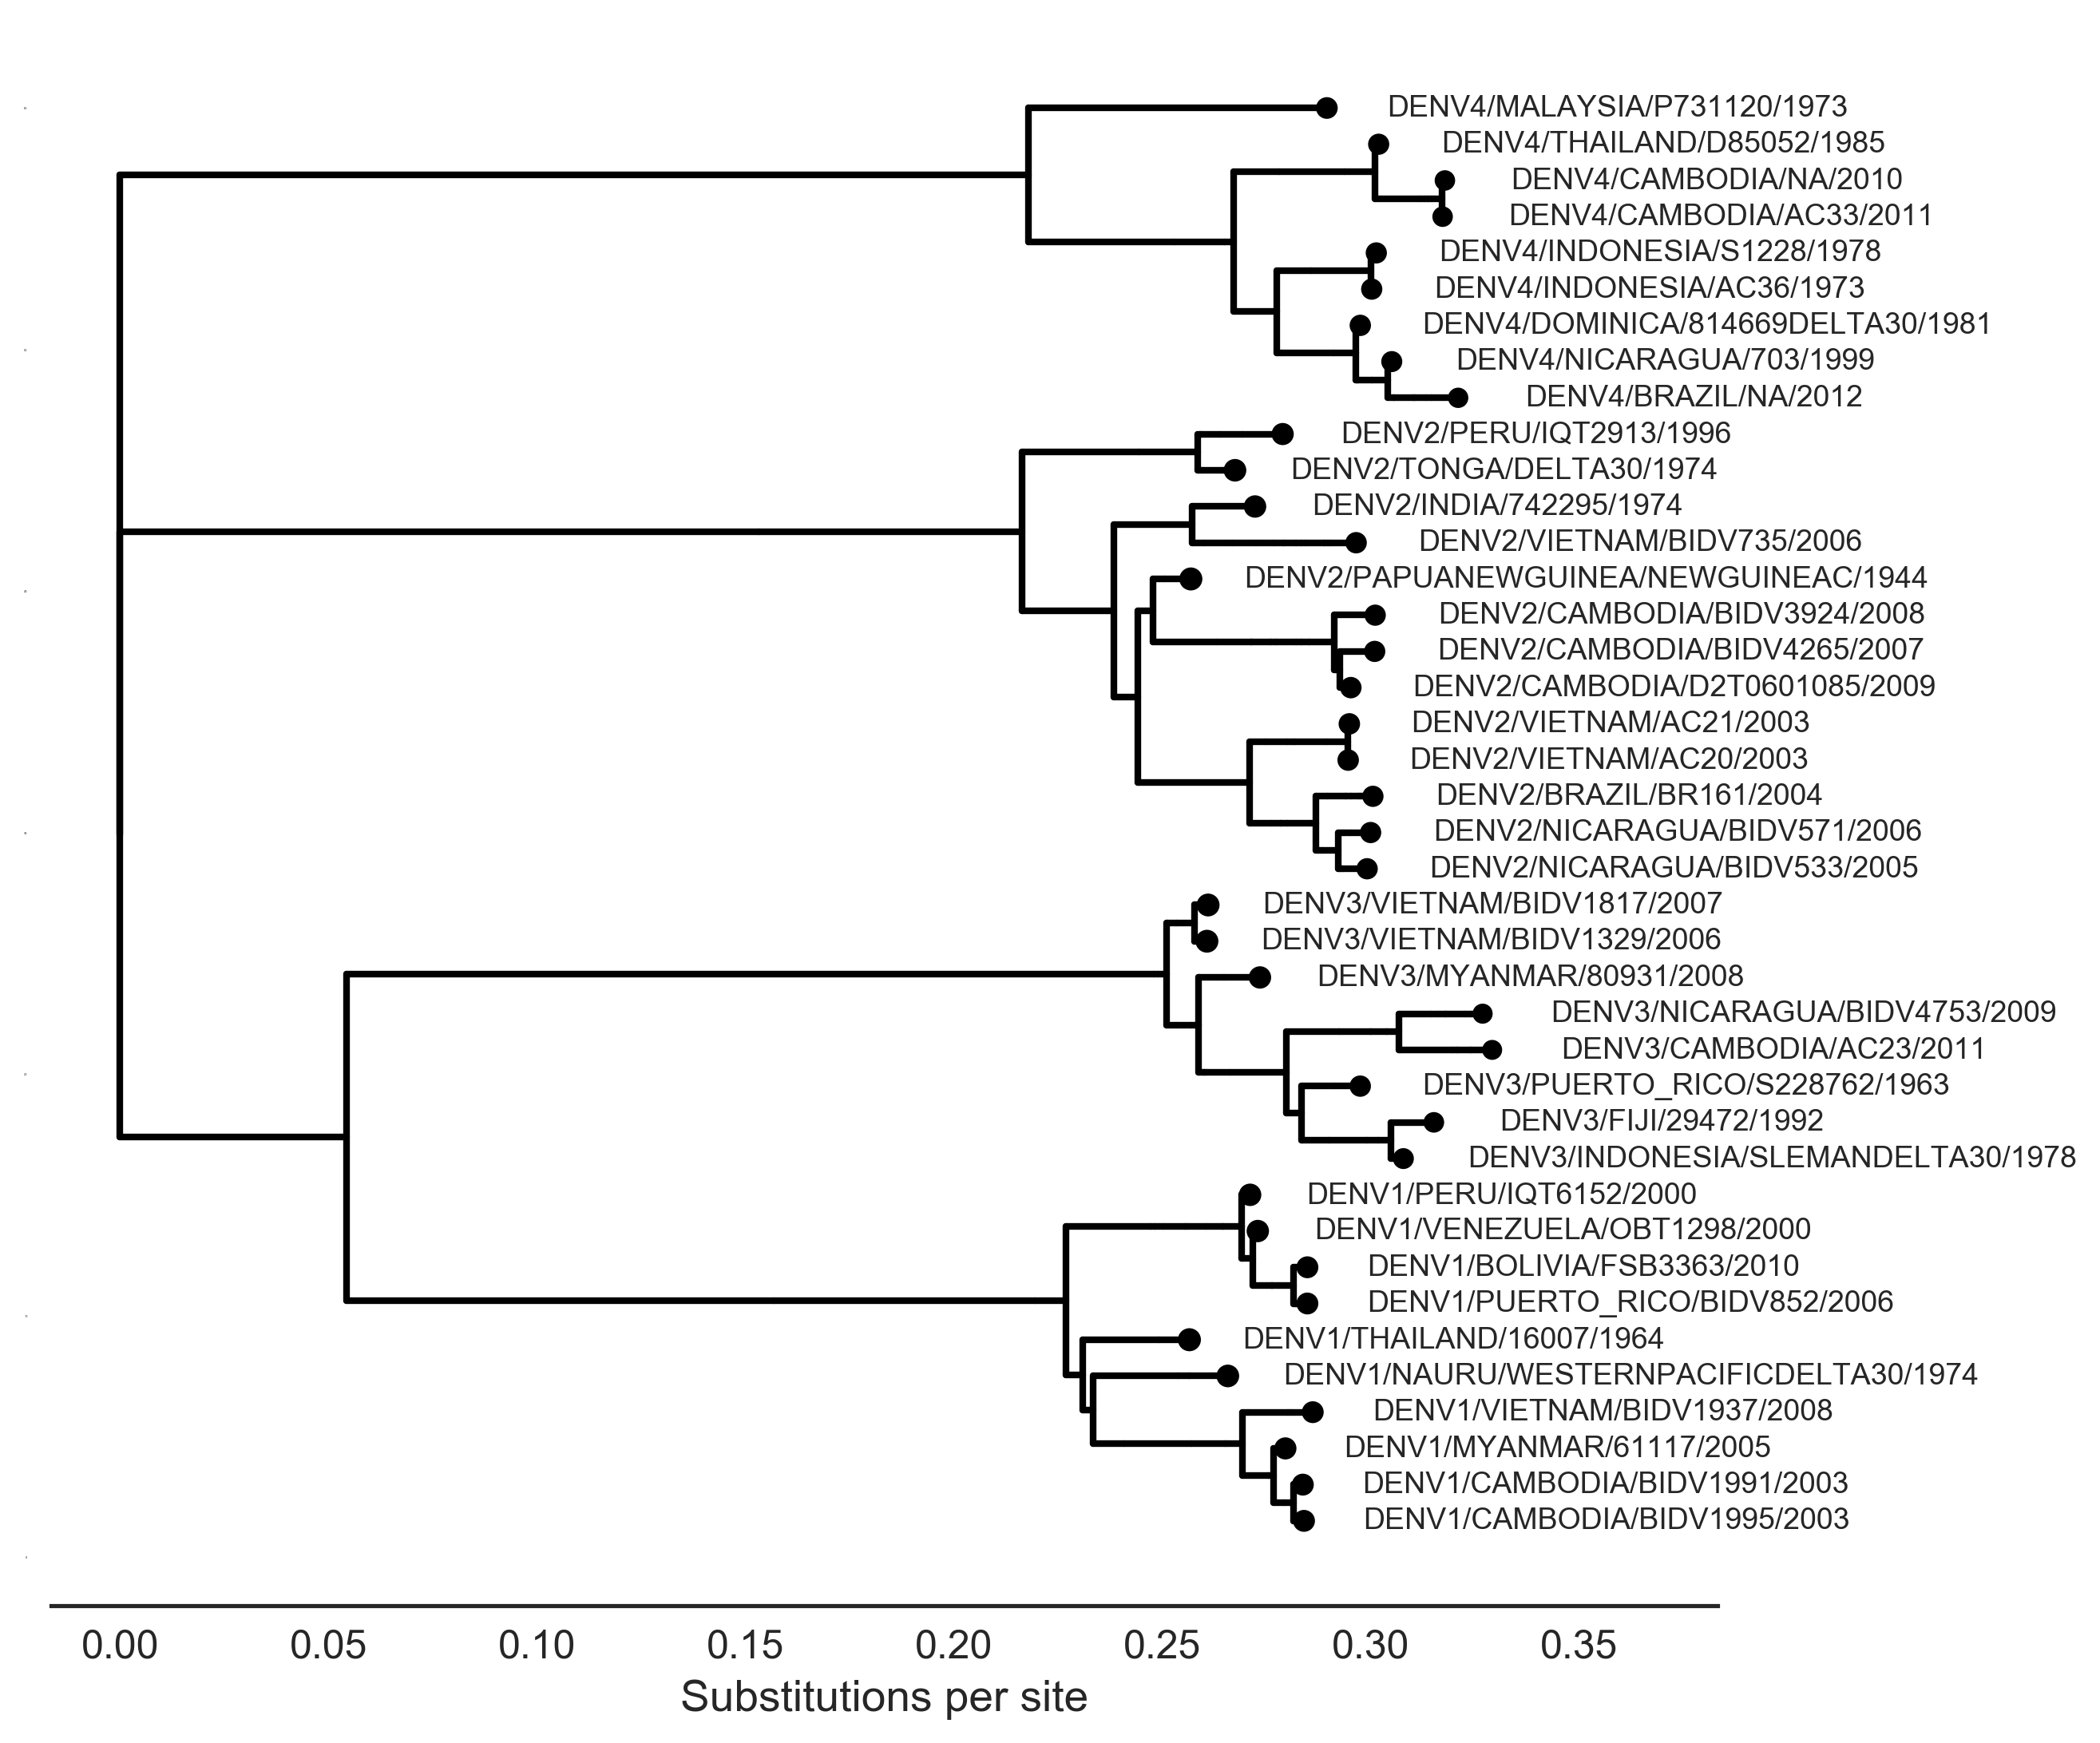
\includegraphics[width=0.75\textwidth]{./png/titered_strains_tree.png}
	\caption{\textbf{Tree of DENV viruses in titer dataset}
  Maximum likelihood phylogeny of all DENV viruses that were included in the titer dataset.
	}
	\label{titered_strains_tree}
\end{figure}

\begin{figure}[h]
\centering
	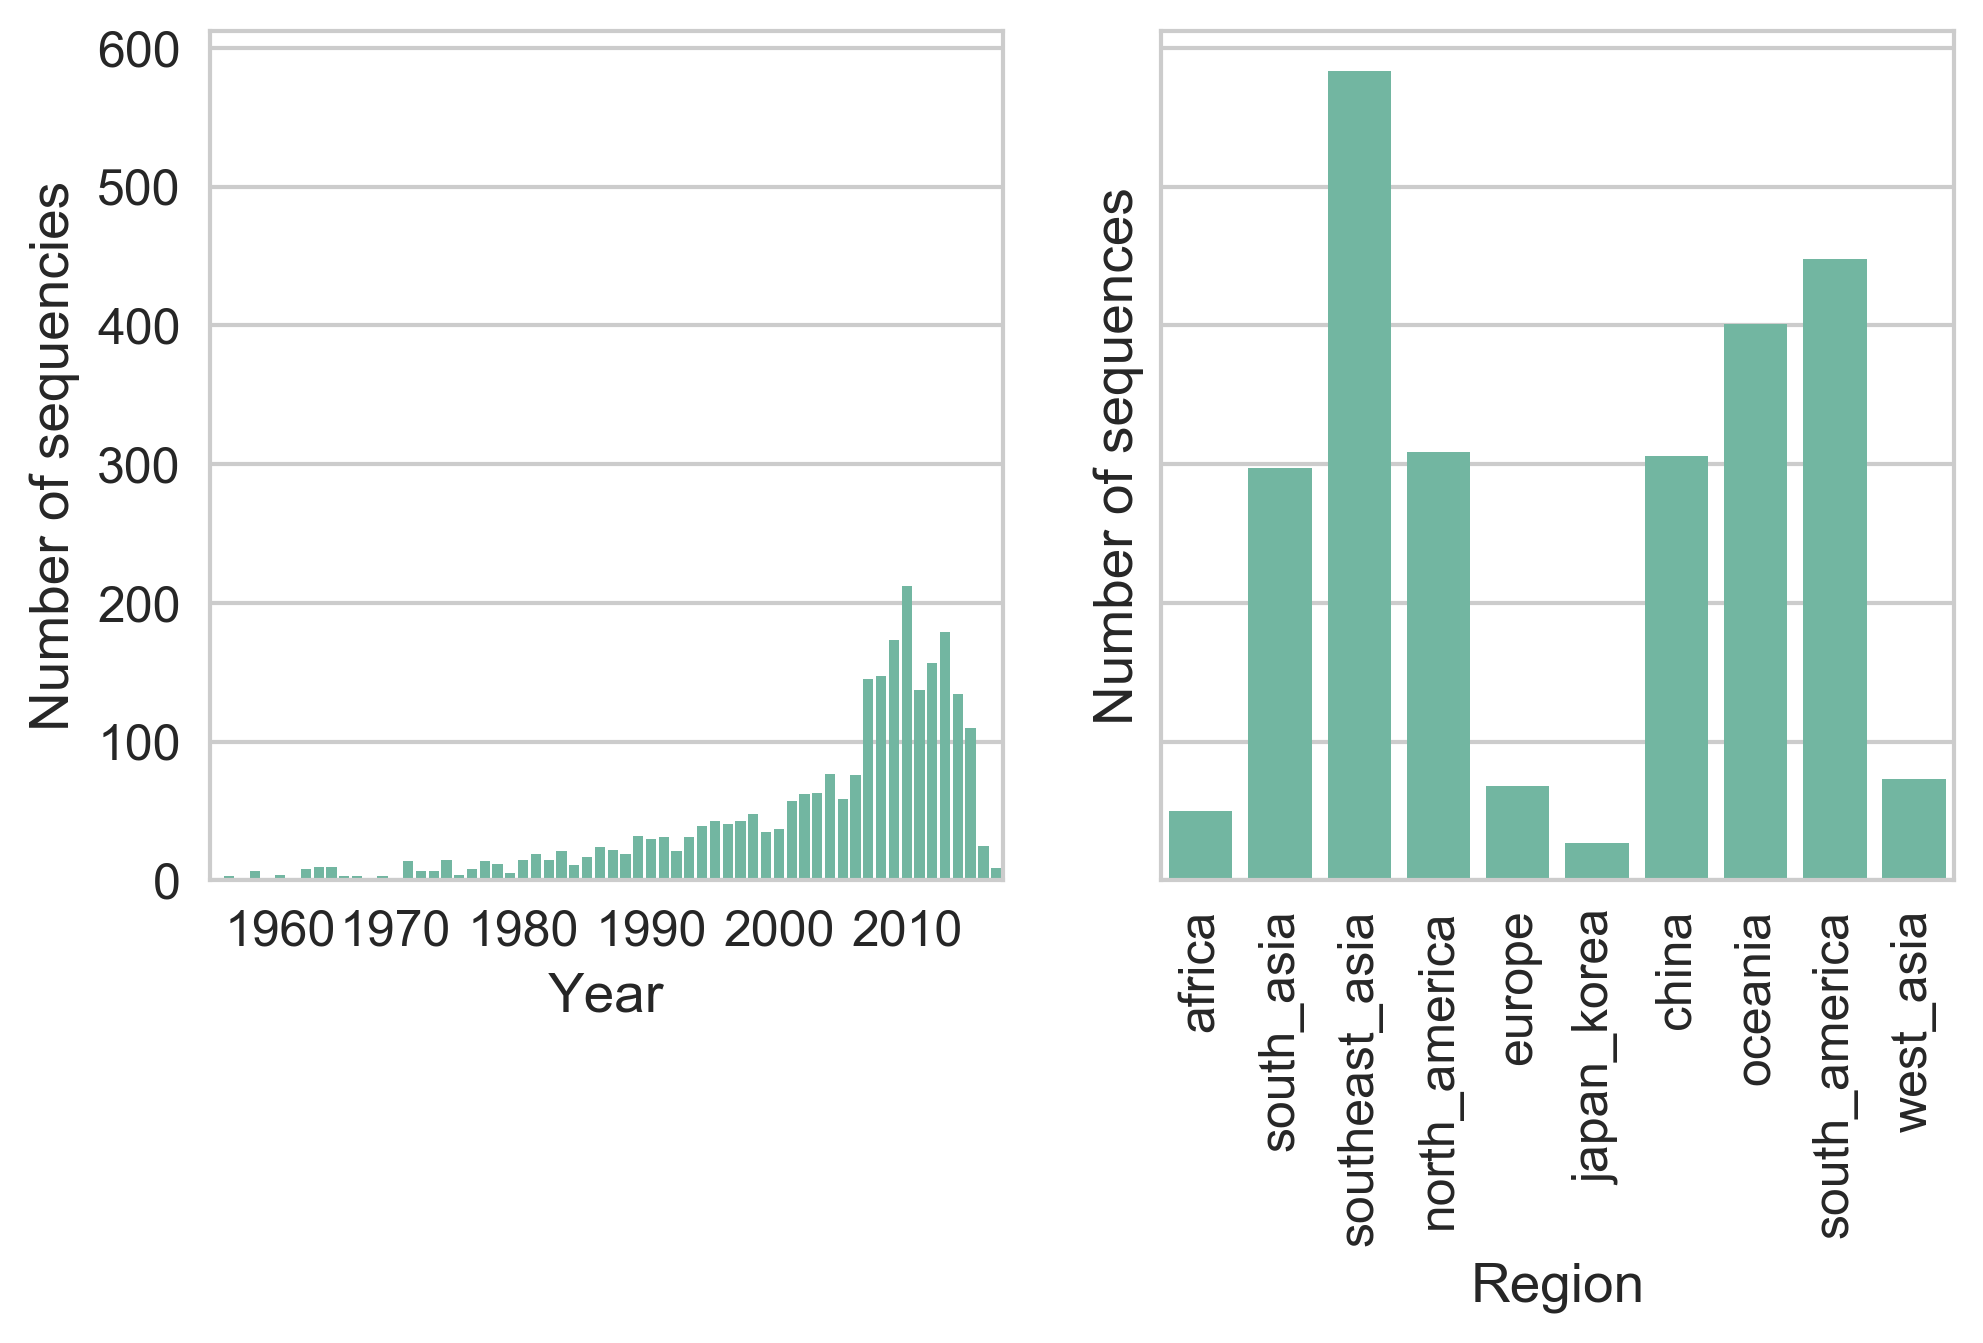
\includegraphics[width=0.75\textwidth]{./png/sequence_distribution.png}
	\caption{\textbf{Sequence dataset distribution}
  Temporal and geographic distribution of sequences included in our dataset after subsampling.
	}
	\label{sequence_distribution}
\end{figure}

\begin{figure}[h]
  \centering
  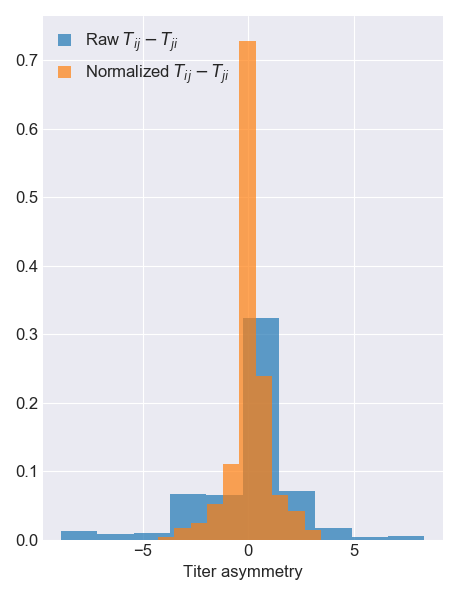
\includegraphics[width=0.5\textwidth]{./png/titer_asymmetry.png}
  \caption{\textbf{Titer value symmetry}
  Some viruses have greater avidity overall, and some sera are more potent overall.
  We normalize for these row and column effects ($v_a$ and $p_b$, respectively) in the titer model.
  Once overall virus avidity and serum potency are accounted for, titers are roughly symmetric (i.e., $D_{ij} \approx D_{ji}$).
  }
\label{titer_asymmetry}
\end{figure}

\begin{figure}[h]
  \centering
  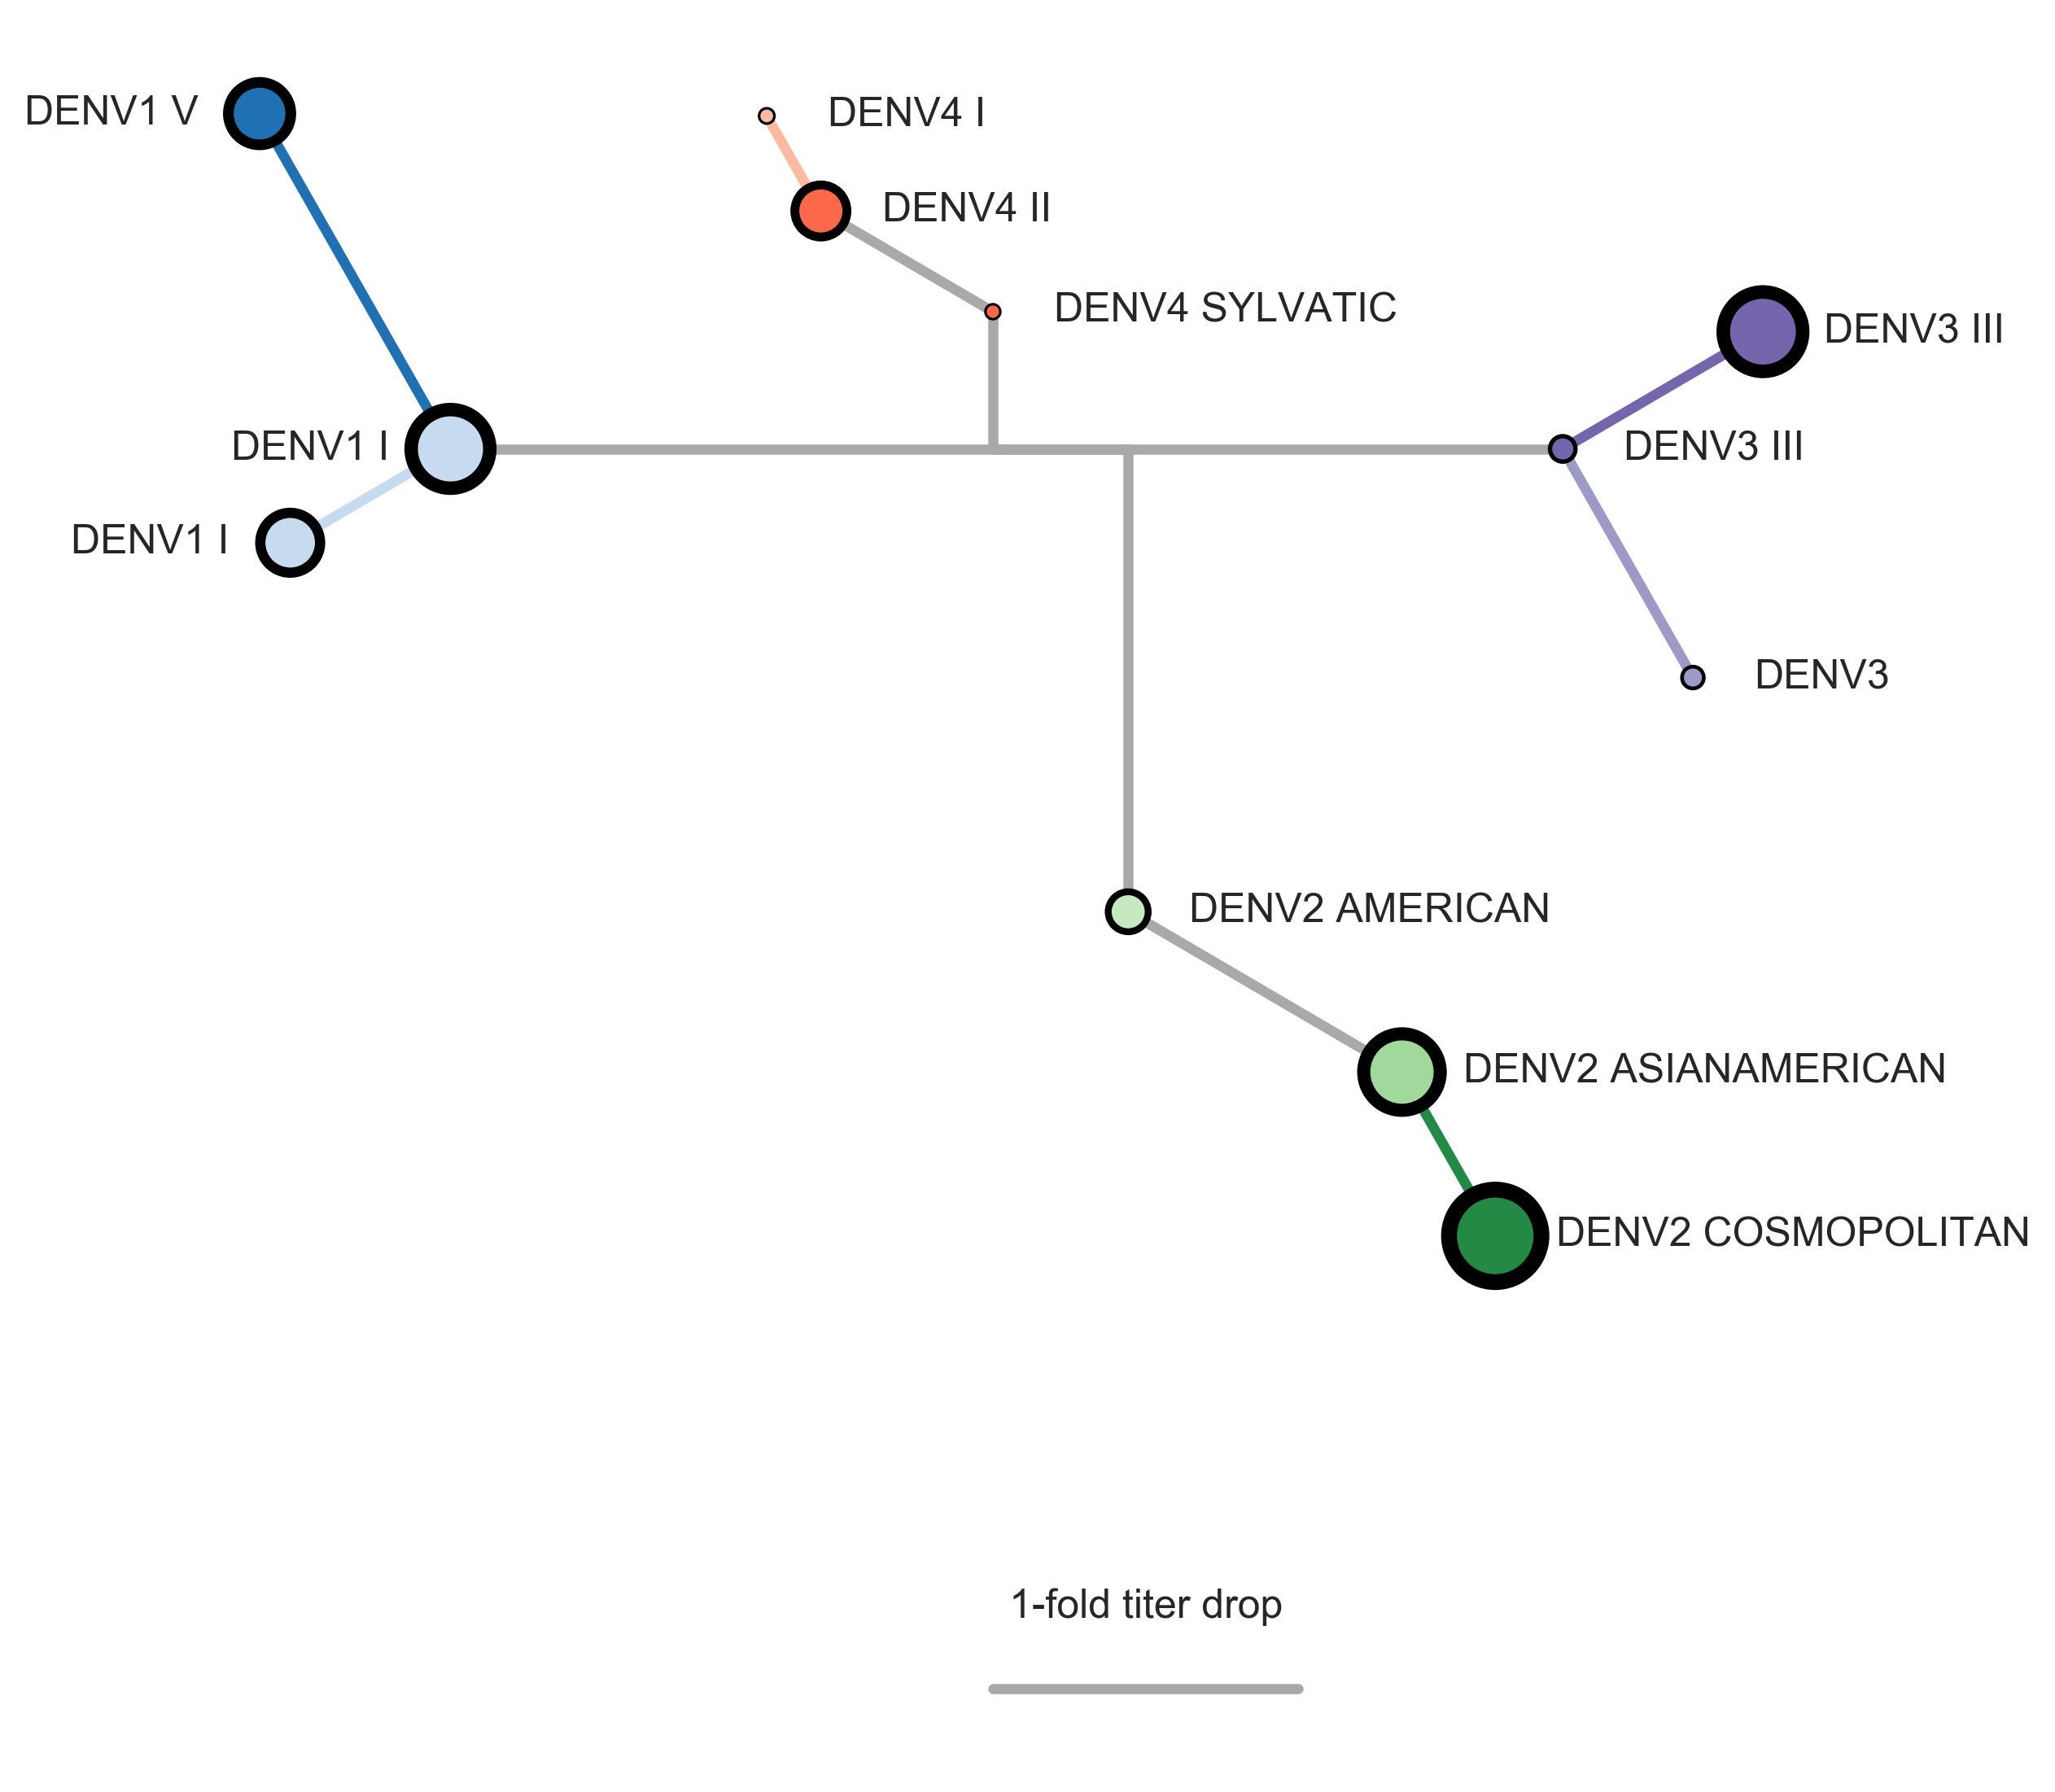
\includegraphics[width=\textwidth]{./png/antigenic_tree_supplement.png}
  \caption{\textbf{Tree of dengue antigenic phenotypes (alternate view)}
As in Figure~\ref{antigenic_tree}, the topology is inferred from a maximum likelihood phylogeny of DENV sequences.
Branch lengths are scaled to represent the $d_b$ assigned to each branch by the `full tree' model of antigenic evolution.
  }
\label{antigenic_tree_supplement}
\end{figure}

\begin{figure}[h]
\centering
	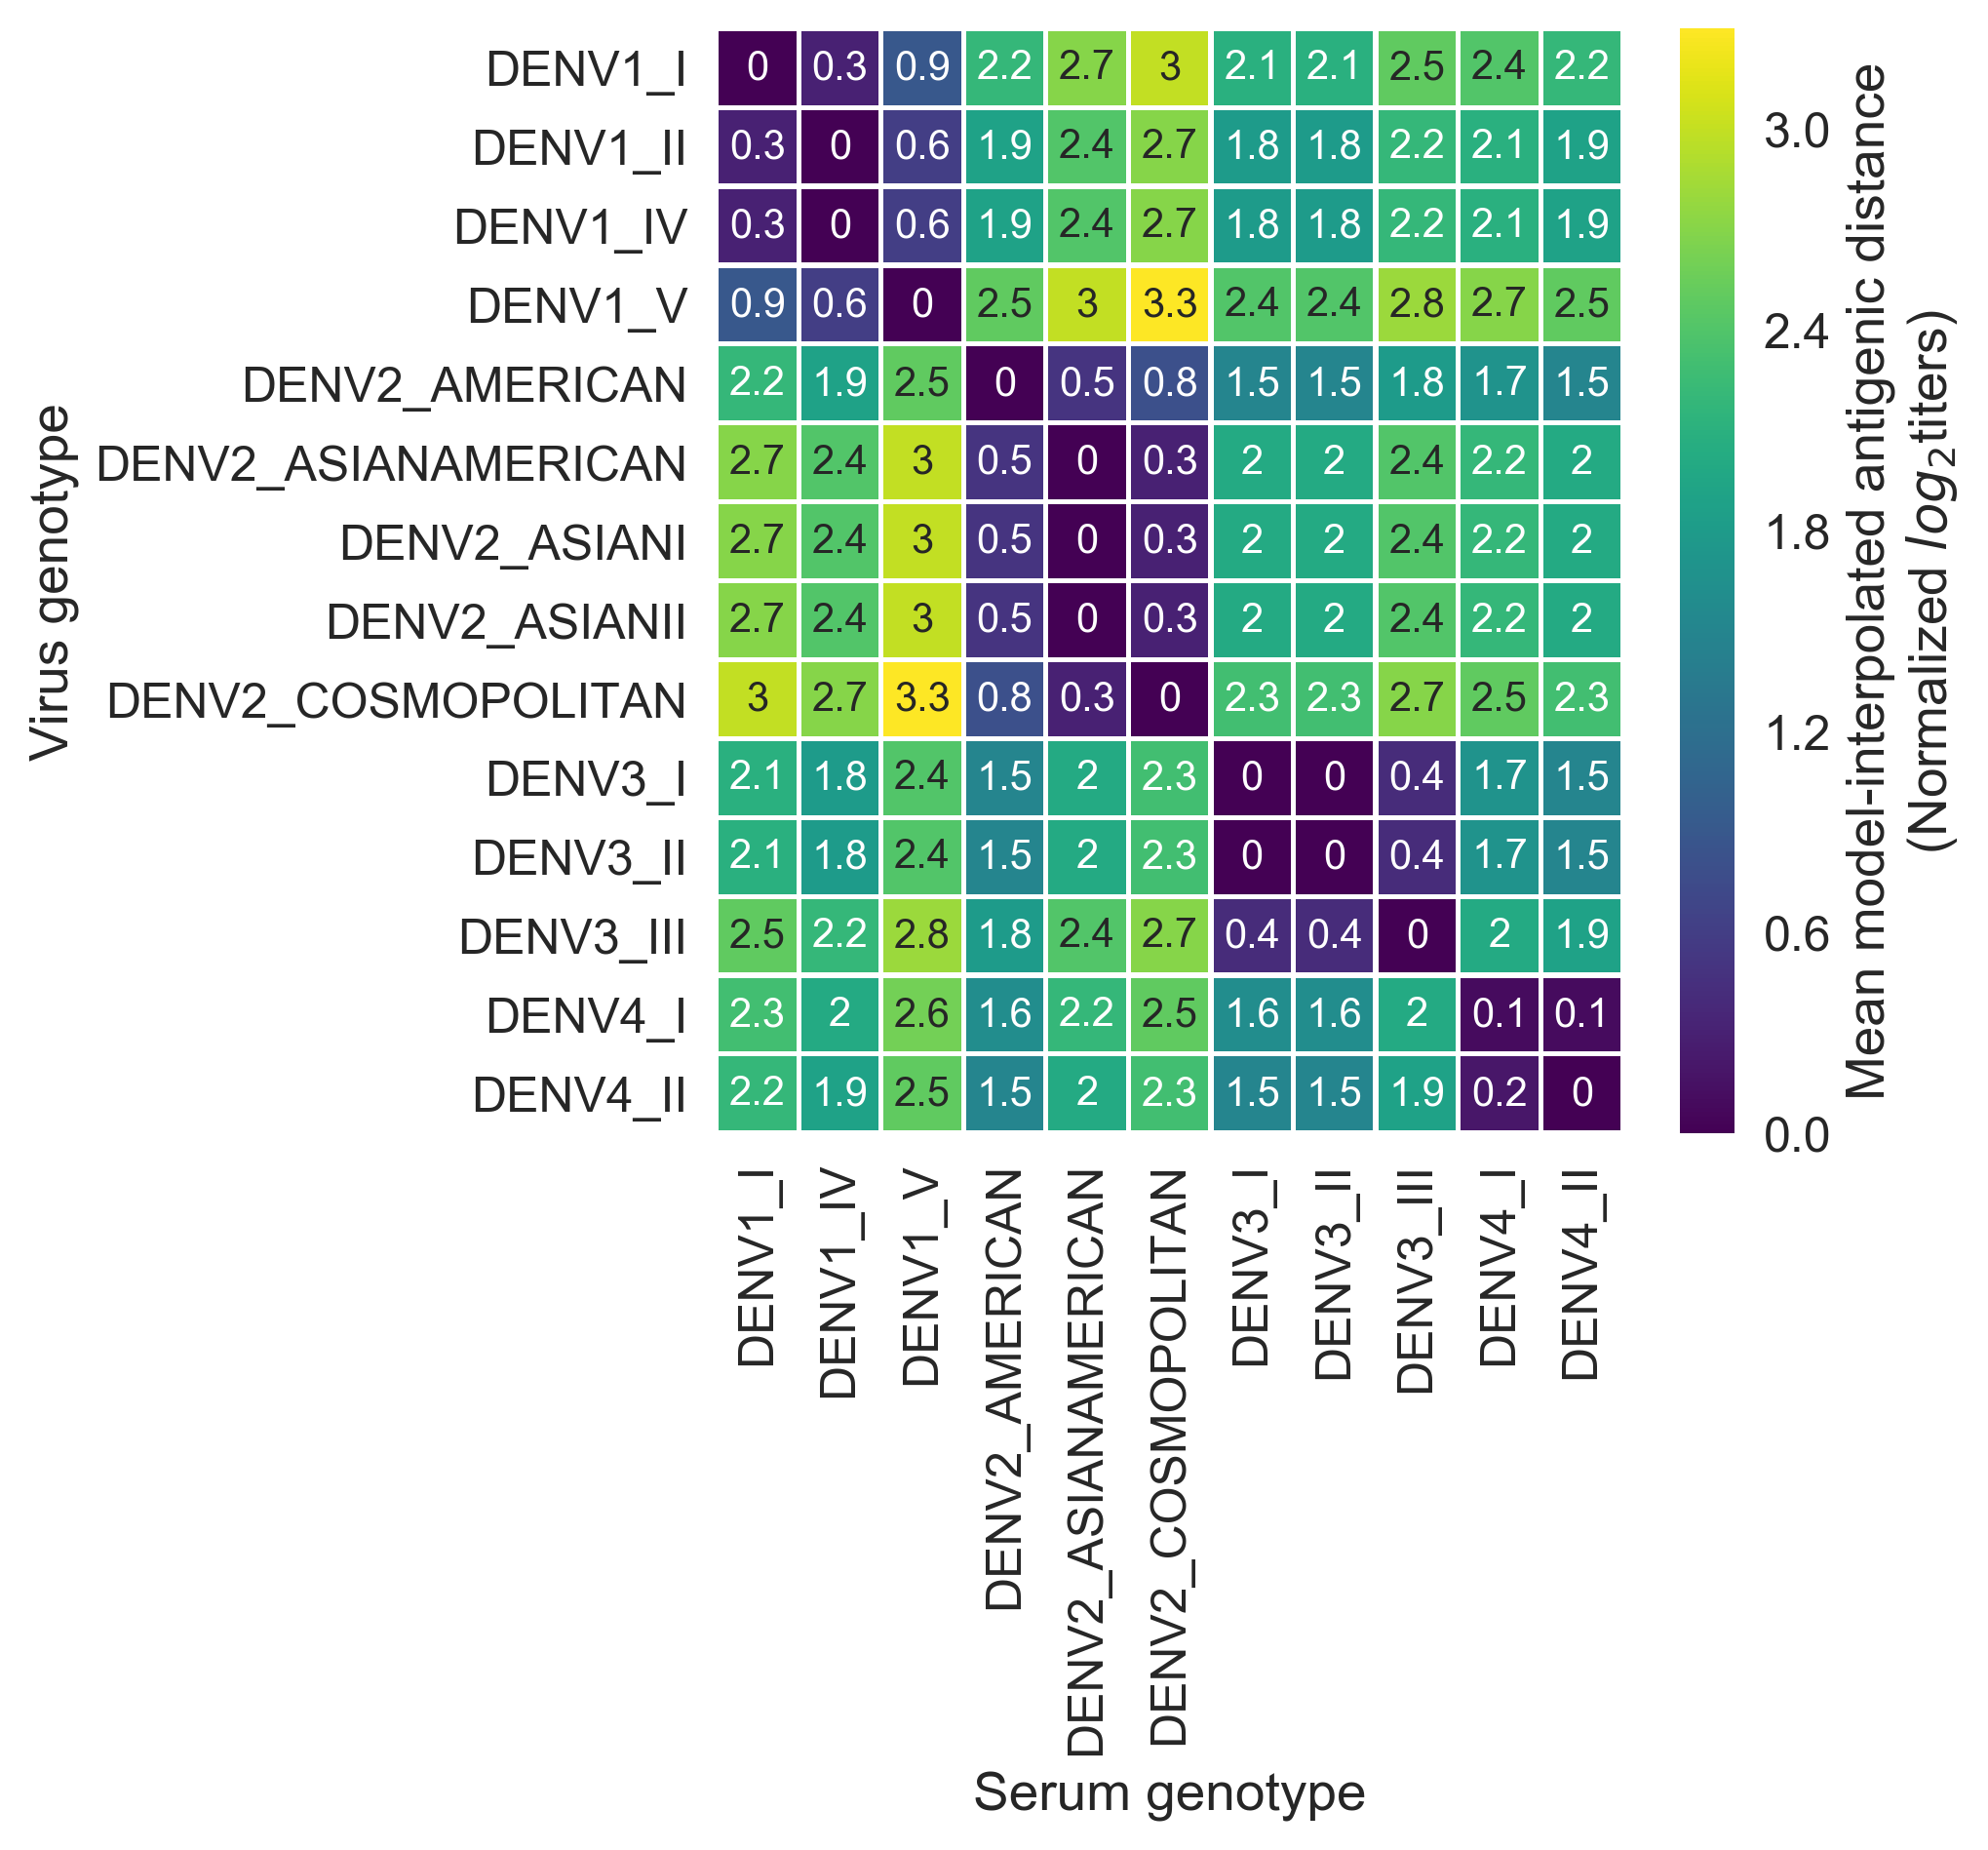
\includegraphics[width=0.75\textwidth]{./png/genotype_dTiter_heatmap.png}
	\caption{\textbf{Titer distance by genotype}
  Values represent the mean interpolated antigenic distance between canonical dengue genotypes (in standardized log$_2$ titer units).
  }
	\label{genotype_dTiter_heatmap}
\end{figure}

% \end{fold}



\end{document}
